% Preámbulo
\PassOptionsToPackage{table}{xcolor}
\documentclass[stu, 12pt, letterpaper, donotrepeattitle, floatsintext]{apa7}
\setcounter{secnumdepth}{5}
\usepackage{fancyvrb}
\usepackage{pmboxdraw}
\usepackage{adjustbox}
\usepackage{caption}
\captionsetup{justification=centering, singlelinecheck=true}
\usepackage[utf8]{inputenc}
\usepackage{comment}
\usepackage{amsmath,amssymb,amsfonts}
\usepackage{marvosym}
\usepackage{graphicx}
\usepackage{pdfpages}
\usepackage{xspace}
\usepackage{blindtext}
\usepackage{ragged2e}
\usepackage{pifont}
\usepackage{xcolor}
\usepackage{forest}
\usepackage{hyperref}
\usepackage{float}

% Fichas de los anexos A y B.
\newcommand{\fichaconsulta}[5]{%
  \par\medskip\noindent
  \begin{tabular}{@{}p{3.2cm}p{10.6cm}@{}}
    \hline
    \textbf{Consulta} & #2 \\
    \textbf{Categoría} & #1 \\
    \textbf{Desafío} & #3 \\
    \textbf{Tools} & #4 \\
    \textbf{Ejecución} & #5 \\
    \hline
  \end{tabular}\par\bigskip
}
\usepackage{booktabs,enumitem,needspace,array,setspace,colortbl}
\usepackage[most]{tcolorbox}
\definecolor{azulanexo}{HTML}{1F3A5F}\definecolor{tblhead}{HTML}{DCE5F0}\definecolor{tblzebra}{HTML}{F4F7FB}
\newtcolorbox{fichap}[3]{enhanced,breakable,colback=azulanexo!5,colframe=azulanexo,colbacktitle=azulanexo,coltitle=white,boxrule=0.6pt,arc=2pt,
  left=5pt,right=5pt,top=3pt,bottom=3pt,fonttitle=\bfseries\small,
  title={Pregunta #1\hfill{\normalfont #2 \;\textbullet\; #3}},before skip=10pt,after skip=3pt}
\newtcolorbox{ejecbox}[5]{enhanced,breakable,colback=white,colframe=black!25,boxrule=0.3pt,arc=0pt,
  borderline west={2.2pt}{0pt}{azulanexo!70},left=6pt,right=5pt,top=2pt,bottom=3pt,
  colbacktitle=azulanexo!12,coltitle=black,fonttitle=\small,
  title={\textbf{Ejecución #1}\hfill Veredicto: \textbf{#2}\\[1pt]{\footnotesize Calidad (C/P/S): \textbf{#5}\hfill Total: #3~s \;\textbullet\; Tools: #4~s}},before skip=2pt,after skip=4pt}
\newcommand{\fichapregunta}[6]{\Needspace*{8\baselineskip}%
 \begin{fichap}{#1}{#2}{#4}
 \textbf{Pregunta.} #3\par\smallskip
 \textbf{Servidor MCP.} #5\par\smallskip
 \textbf{Referencia.} #6
 \end{fichap}}
\newcommand{\ejecucion}[7]{\begin{ejecbox}{#1}{#2}{#3}{#4}{#5}
 {\footnotesize\textbf{Tools usadas.} #6}\par\smallskip
 {\small #7}
 \end{ejecbox}}
\newcommand{\notaeval}[1]{\par\vspace{1pt}{\footnotesize\itshape\textbf{Nota de evaluación.} #1}\par\vspace{4pt}}
\usepackage[normalem]{ulem}
\usepackage[spanish]{babel}
\addto\captionsspanish{\renewcommand{\tablename}{Tabla}}
\setlength{\parskip}{0.6em plus 0.1em minus 0.1em}
\setlength{\parindent}{0pt}
\selectlanguage{spanish}
\useunder{\uline}{\ul}{}
\newcommand{\myparagraph}[1]{\paragraph{#1}\mbox{}\\}



\usepackage[american,cuteinductors,smartlabels]{circuitikz}
\usetikzlibrary{calc}
\ctikzset{bipoles/thickness=1}
\ctikzset{bipoles/length=1.1cm}
\ctikzset{bipoles/diode/height=.3}
\ctikzset{bipoles/diode/width=.2}
\ctikzset{tripoles/nigbt/height=1.4}
\ctikzset{tripoles/nigbt/width=1}
\ctikzset{bipoles/vsourceam/height/.initial=.7}
\ctikzset{bipoles/vsourceam/width/.initial=.7}
\tikzstyle{every node}=[font=\large]
\tikzstyle{every path}=[line width=1.5pt,line cap=round,line join=round]
\usepackage{tikz}
\renewcommand\refname{\large\textbf{Referencias}}
\usepackage[
	backend=biber,
	style=ieee,
	sorting=none,
	url=true,
	doi=true,
	eprint=false
]{biblatex}
\addbibresource{10_references.bib}
\usetikzlibrary{shapes,arrows}
\usepackage{afterpage}
\tikzstyle{blockp} = [draw, rectangle, minimum height=22em, minimum width=8em] %fill=blue!20
\tikzstyle{block_kalman} = [draw, rectangle, minimum height=4em, minimum width=8em] %fill=blue!20
\tikzstyle{block} = [draw, rectangle, minimum height=2em, minimum width=4em] %fill=blue!20
\tikzstyle{sum} = [draw, circle  , minimum size=0.5cm, node distance=2cm]
\tikzstyle{input} = [coordinate]
\tikzstyle{output} = [coordinate]
\tikzstyle{pinstyle} = [pin edge={to-,thin,black}]




% Portada
\thispagestyle{empty}
\title{\Large Título del documento}
\author{Autor(a) \\Autor(a) \\Autor(a)} % (autores separados, consultar al docente)
% Manera oficial de colocar los autores:
%\author{Autor(a) I, Autor(a) II, Autor(a) III, Autor(a) X}
\affiliation{Nombre de la institución}
\course{Código del curso: Nombre del curso}
\professor{Nombre del docente}
\duedate{Fecha}







\begin{document}

\markright{Integración de LLM a arquitectura UNS para analítica de datos en Industria 4.0}
\pagestyle{myheadings}


\begin{titlepage}
\begin{center}

Integración de una herramienta basada en modelos de lenguaje de gran tamaño a una arquitectura UNS para analítica de datos en industria 4.0

\vspace*{3cm}

Norbey Camilo Infante Villamil

\vspace*{3cm}

Trabajo de investigación para optar por el título de Magíster en Ingeniería de Telecomunicaciones


\vspace*{2cm}


Director

Juan Manuel Rey López

Doctor en Ingeniería Electrónica
\vfill


Universidad Industrial de Santander

Facultad de Ingenierías Fisicomecánicas

Escuela de Ingenierías Eléctrica, Electrónica y de Telecomunicaciones

Bucaramanga

2026

\end{center}

\end{titlepage}



\pagenumbering{roman}


    % Contenido
\renewcommand\contentsname{\largeÍndice}
\tableofcontents
\setcounter{tocdepth}{2}
\newpage
    % Fíguras
\renewcommand{\listfigurename}{\largeÍndice de fíguras}
\listoffigures
\newpage
    % Tablas
\renewcommand{\listtablename}{\largeÍndice de tablas}
\listoftables
\newpage


\begin{center}
    {\large \textbf{Resumen}}
\end{center}
\justify
\textcolor{blue}{Pendiente: La Cuarta Revolución Industrial, o Industria 4.0, está redefiniendo el sector manufacturero mediante la integración de tecnologías avanzadas como el Internet Industrial de las Cosas (IIoT), la inteligencia artificial (IA) y los sistemas ciberfísicos. Un elemento clave en esta transformación es el \textit{Unified Namespace (UNS)}, una arquitectura que optimiza la gestión de datos en tiempo real, superando las limitaciones de integración y escalabilidad de las estructuras tradicionales. Sin embargo, su adopción generalizada se ha visto obstaculizada por la falta de documentación técnica detallada y metodologías de implementación bien definidas. Este estudio revisa los conceptos fundamentales del UNS, analiza sus metodologías de implementación y compara diferentes enfoques de diseño. Para validar su aplicación, se desarrolla un caso práctico basado en una plataforma de entrenamiento IIoT que utiliza el protocolo de comunicación MQTT Sparkplug B. Este trabajo no solo proporciona una referencia estructurada para la comunidad académica, sino que también ofrece lineamientos prácticos para la industria, facilitando la comprensión y adopción del UNS en entornos productivos.}
\newpage
\begin{center}
    {\large \textbf{Abstract}}
\end{center}
\justify
\textcolor{blue}{Pendiente: The Fourth Industrial Revolution, or Industry 4.0, is transforming the manufacturing sector by integrating advanced technologies such as the Industrial Internet of Things (IIoT), artificial intelligence (AI), and cyber-physical systems. A key enabler of this transformation is the \textit{Unified Namespace (UNS)}, an architecture that optimizes real-time data management, overcoming the integration and scalability challenges of traditional structures. However, its widespread adoption has been limited by the lack of comprehensive technical documentation and well-defined implementation methodologies. This study reviews the fundamental concepts of UNS, analyzes its implementation methodologies, and compares different design approaches. To validate its application, a case study is developed using an IIoT training platform based on the MQTT Sparkplug B communication protocol. This work not only provides a structured reference for the academic community but also offers practical guidelines for industry stakeholders, facilitating the understanding and adoption of UNS in manufacturing environments.}

\newpage
% Cuerpo
\pagenumbering{arabic}


%%%%% PROPUESTA DE ÍNDICE %%%%%

% 1) Introducción
%   > Aterrizamos al contexto (industria 4.0 -> UNS)
%   > Formulación del problema: falta de documentación -> falta de comparaciones entre las propuestas

% 2) UNS -> explicar el concepto
% Técnicas

% 3) Caso de estudio
% Aplicación
% Herramienta de comparación

% 4) Resultados y análisis

% 5) Conclusiones



\label{chap:Intro}


\cleardoublepage

\setcounter{section}{-1}
\section{Introducción}

En la última década, la transformación digital ha dejado de ser tendencia para convertirse en una necesidad estratégica para las organizaciones. Este proceso involucra la adopción de tecnologías emergentes para rediseñar operaciones, optimizar recursos y mejorar la adaptación frente a entornos cada vez más volátiles. En el contexto de la Cuarta Revolución Industrial (Industria 4.0), la convergencia de tecnologías como el Internet Industrial de las Cosas (IIoT), la inteligencia artificial (IA), la computación en la nube y la analítica avanzada está redefiniendo los modelos productivos y de gestión en todos los niveles de las organizaciones.



Según el Foro Económico Mundial, las empresas que adoptan estas tecnologías no solo logran mejoras en su eficiencia operativa, sino que también fortalecen su capacidad de respuesta ante crisis, interrupciones logísticas o cambios bruscos en la demanda global \cite{wef1}. En este sentido, la transformación digital se convierte en pieza clave para habilitar la resiliencia organizacional. Una evidencia particular es presentada en el artículo \cite{scd1}, donde se analizaron datos empresariales para evaluar el impacto de la transformación digital sobre la resiliencia de las cadenas de suministro. Los resultados muestran que la digitalización no solo tiene un efecto directo positivo en la capacidad de adaptación organizacional, sino que además fortalece la transparencia en la cadena de suministro, lo que contribuye a una mayor estabilidad frente a disrupciones externas. Aunque América Latina enfrenta desafíos en infraestructura digital y formación de talento, informes de la CEPAL subrayan que las empresas que han avanzado en procesos de transformación digital en esta región muestran una mayor capacidad de recuperación económica y adaptación estratégica frente a entornos cambiantes \cite{cepaL}.

En paralelo, el avance de la Industria 4.0 también plantea retos en el ámbito laboral. Según el Foro Económico Mundial, la implementación de tecnologías como la robótica, la automatización y la IA está transformando no solo los procesos productivos, sino también las funciones de los trabajadores dentro de las organizaciones. Esta transformación exige una actualización constante de habilidades técnicas y digitales, así como una reconfiguración de los roles laborales tradicionales para adaptarse a entornos cada vez más conectados \cite{wef2}.

A pesar de estos avances, muchas industrias aún operan con arquitecturas tradicionales, como la ISA-95, que, aunque están ampliamente consolidadas, pueden limitar la interoperabilidad y dificultar la integración con nuevas tecnologías. Frente a esto, la arquitectura Unified Namespace (UNS) emerge como una alternativa para centralizar, estandarizar y estructurar el flujo de datos en tiempo real. Esta arquitectura facilita la integración entre sistemas, elimina silos de información y permite el despliegue eficiente de soluciones avanzadas en analítica de datos.


\subsection{\centering Justificación}

La transformación digital es un factor determinante en la evolución de los entornos industriales hacia modelos más inteligentes, flexibles y resilientes. La ndustria 4.0 ha introducido tecnologías que permiten una automatización avanzada y una integración más profunda entre los sistemas físicos y digitales. No obstante, aún persisten desafíos importantes en cuanto a la forma en que las empresas acceden, estructuran y explotan eficientemente la información generada en sus procesos operativos.


Uno de los principales obstáculos radica en la fragmentación y dispersión de los datos, tanto estructurados como no estructurados. El UNS surge como una solución para centralizar y estandarizar el flujo de datos en tiempo real. Aunque implementar una arquitectura UNS mejora la accesibilidad y la integración de los datos, por sí sola no garantiza el aprovechamiento inteligente de la información. Para lograr un verdadero valor agregado, es necesario incorporar herramientas que permitan interpretar los datos de forma eficiente.


En este sentido, los Modelos de Lenguaje de Gran Tamaño (LLMs) ofrecen un potencial transformador. Gracias a su capacidad para comprender lenguaje natural, generar texto coherente y realizar búsquedas semánticas sobre grandes volúmenes de información, los LLMs pueden actuar como una capa de inteligencia contextual sobre la arquitectura UNS. Esta sinergia habilita nuevas formas de interacción entre los operadores y los sistemas industriales, permitiendo, por ejemplo, responder consultas técnicas mediante lenguaje natural, generar reportes automatizados y acceder a conocimiento distribuido sin necesidad de navegar por múltiples fuentes.


\subsection{\centering Descripción del proyecto}
En el contexto industrial actual, las empresas generan y consumen grandes volúmenes de información provenientes de fuentes heterogéneas. Esta información abarca tanto datos estructurados (registros de sistemas ERP, MES, SCADA, y bases de datos) como datos no estructurados (manuales técnicos, reportes operativos, y documentos de mantenimiento). Uno de los principales desafíos es la fragmentación, dispersión y falta de estandarización de estos datos. En este escenario, la arquitectura UNS surge como una solución para centralizar, estandarizar y visualizar de manera unificada la información de todos los niveles de la operación en tiempo real. No obstante, la simple centralización no garantiza el aprovechamiento inteligente de la información. Se requieren herramientas que permitan realizar análisis semánticos, búsquedas contextuales y generación automatizada de conocimiento útil. Los LLMs ofrecen un potencial transformador gracias a su capacidad para comprender lenguaje natural, extraer significado de textos no estructurados y generar respuestas contextualizadas, por lo que tienen la capacidad de actuar como una capa de ``inteligencia'' sobre la arquitectura UNS. El presente proyecto de investigación tiene como propósito proponer un mecanismo para la integración efectiva de herramientas basadas en Modelos de LLMs dentro de arquitecturas UNS aplicadas al contexto de la Industria 4.0. La investigación busca determinar cómo la incorporación de estas herramientas puede potenciar las capacidades del UNS, permitiendo funcionalidades avanzadas como búsquedas inteligentes, consultas semánticas, generación automática y dinámica de reportes en entornos industriales reales.


\subsection{\centering Objetivos}
A continuación, se presentan el objetivo general y los objetivos específicos del trabajo de investigación.


\textbf{Objetivo general}

Integrar una herramienta basada en modelos de lenguaje de gran tamaño para la analítica de datos de una arquitectura Unified Namespace aplicada a un caso de industria 4.0.

\vspace{0.5cm}


\textbf{\centering Objetivos específicos}
\begin{itemize}
    \item \textbf{OE1:} Caracterizar un caso de estudio en Industria 4.0, identificando los requerimientos y desafíos específicos de analítica de datos.

    \item \textbf{OE2:} Diseñar e implementar una arquitectura Unified Namespace, estableciendo la estructura de datos.

    \item \textbf{OE3:} Seleccionar una herramienta basada en modelo de lenguaje de gran tamaño, considerando criterios de adaptabilidad al caso de estudio.

    \item \textbf{OE4:} Integrar la herramienta de lenguaje de gran tamaño a la arquitectura Unified Namespace, proporcionando al modelo el contexto correspondiente al caso de estudio.

    \item \textbf{OE5:} Validar el funcionamiento del sistema integrado mediante métricas de desempeño.

\end{itemize}

\subsection{\centering Esquema del trabajo de investigación}

Este trabajo de investigación está organizado de la siguiente manera:

\color{blue}
\begin{itemize}
    \item  \textbf{Capítulo~\ref{cap:caso_estudio}:} Caracterización del caso de estudio de Industria 4.0
    \item  \textbf{Capítulo~\ref{tecnicasdiseñouns}:} Implementación de arquitectura UNS
    \item  \textbf{Capítulo~\ref{seleccionllm}:} Selección del mecanismo de integración y herramienta LLM
    \item  \textbf{Capítulo~\ref{implementacionintegracion}:} Integración de la herramienta LLM a la arquitectura UNS
    \item  \textbf{Capítulo~\ref{validacionsistema}:} Validación del sistema integrado

\end{itemize}
\color{black}
\clearpage\phantomsection

\label{chap:capitulo1}
 


\section{Capítulo 1: Caracterización del caso de estudio en Industria 4.0}
\label{cap:caso_estudio}

Este capítulo caracteriza el caso de estudio que sirve de base al presente trabajo, inspirado en un proyecto de integración IIoT desarrollado por la empresa aliada DAUTOM S.A.S. en el sector molinero. A continuación se describe el contexto del proyecto, el proceso productivo y su flujo operacional.

\subsection{Contexto del caso de estudio}

El caso de estudio parte de un proyecto real de integración IIoT desarrollado por \href{https://www.dautom.com.co/}{DAUTOM S.A.S.} en Barranquilla, Colombia. El proyecto conectó las áreas de empaque de harina de maíz y de trigo a una plataforma MES (Manufacturing Execution System), donde la información recolectada se emplea para calcular rendimientos de proceso, evaluar la disponibilidad de las máquinas y controlar la calidad del producto.

\subsection{Proceso y flujo operacional del área de empaque}

Esta área toma la harina producida en los molinos y la envasa para su comercialización. Al ser el punto final de la cadena antes de la distribución al cliente, se convierte en un nodo crítico de medición: cualquier pérdida de disponibilidad o calidad se traduce directamente en producto no despachado.

Cada área de empaque —trigo y maíz— opera con dos líneas de producción independientes, identificadas como Línea A y Línea B. El flujo fisico del producto inicia una vez el material sale de los molinos y llega a silos de almacenamiento temporal; a partir de ahí, cada línea ejecuta los siguientes pasos:

\begin{enumerate}
    \item \textbf{Empacado:} el producto se traslada mediante sistemas de transporte neumático y mecánico hacia las máquinas encargadas de envasar la harina en bolsas de una libra o de un kilo. Cada línea dispone de \textbf{2 empacadoras} (cuatro por área), lo que permite mantener la continuidad operativa ante mantenimientos o fallas en una de ellas.
    
    \item \textbf{Enfardado:} las bolsas se agrupan y embalan en fardos mediante la enfardadora, equipo que facilita el manejo, almacenamiento y transporte del producto. Cada línea cuenta con \textbf{1 enfardadora} (dos por área). La cantidad de bolsas del fardo depende de la presentación: para libra, cada fardo contiene 24 unidades; para kilo, 20 unidades.
\end{enumerate}

Este proceso se ejecuta siempre dentro del contexto de una orden de producción (\textit{Work Order}, WO): un registro creado en el MES sobre la plataforma Ignition, a nivel de línea, que especifica el producto a envasar (harina de trigo o de maíz), la presentación (libra o kilo) y la cantidad meta de unidades. La ejecución de una WO, con sus tiempos reales de inicio y fin, se denomina \textit{corrida}. Una vez inicia la corrida, el sistema vincula automáticamente los datos capturados en planta con la WO correspondiente, y registra en tiempo real los eventos del ciclo productivo: inicio, pausas, reanudaciones y cierre. Esta vinculación entre los datos operativos y el contexto de negocio de cada corrida es lo que permite, más adelante, calcular indicadores como el cumplimiento de la orden o la eficiencia de línea, y es también uno de los elementos que la herramienta LLM deberá interpretar para responder consultas que combinen información en tiempo real con el estado de la producción planificada.

    La figura \ref{fig:flujo_empaque} muestra esquema que representa el flujo operativo descrito anteriormente. 
    
    \begin{figure}[H]
        \centering
        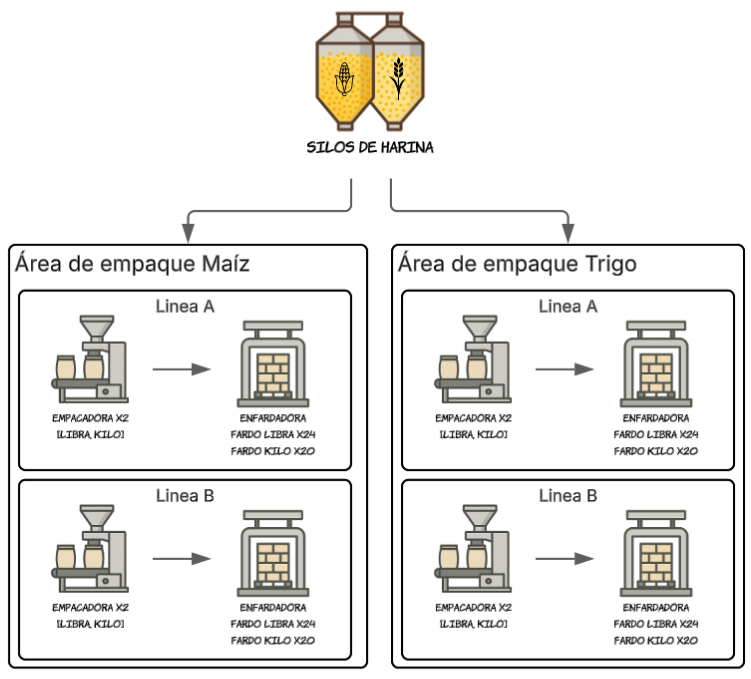
\includegraphics[width=1\textwidth]{Figuras/FlujoMolineria.png}
        \caption{Esquema del flujo operativo del caso de estudio.}
        \label{fig:flujo_empaque}
    \end{figure}

\subsection{Adquisición de datos}

La infraestructura de adquisición de datos de las áreas de empaque se basa en una arquitectura distribuida de controladores industriales que capturan información operativa en tiempo real y la transmiten hacia el centro de control. La Figura \ref{fig:arquitectura_iiot} ilustra esta arquitectura IIoT para las dos áreas del caso de estudio.

\begin{figure}[H]
    \centering
    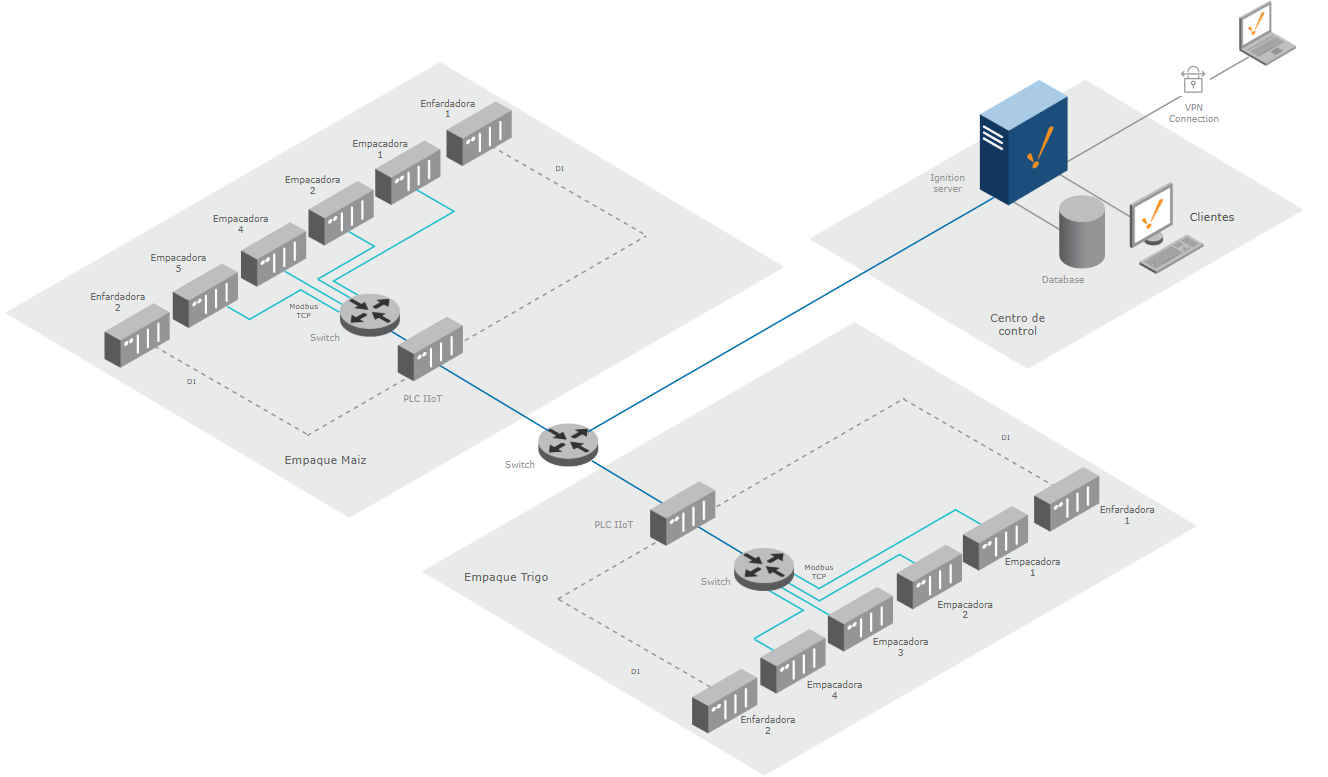
\includegraphics[width=1\textwidth]{Figuras/diagrama_arquitectura.png}
    \caption{Arquitectura IIoT del caso de estudio \textcolor{red}{Falta actualizar esta figura}.}
    \label{fig:arquitectura_iiot}
\end{figure}

\subsubsection{Datos capturados en planta}

\begin{enumerate}
    \item \textbf{Empacadoras:} cada una cuenta con un PLC Omron dedicado que gestiona su lógica de control y captura las siguientes variables:
    \begin{itemize}
        \item \textbf{Conteo de bolsas producidas:} contador acumulado de unidades empacadas.
        \item \textbf{Tiempo de ciclo:} tiempo requerido para completar el empaque de una unidad.
        \item \textbf{Estado de la máquina:} marcha, paro, alarma o mantenimiento.
    \end{itemize}
    Como cada línea dispone de dos empacadoras, cada área cuenta con cuatro PLCs Omron.

    \item \textbf{Enfardadoras:} a diferencia de las empacadoras, solo se tiene acceso a sus señales de entrada/salida (I/O), que proporcionan:
    \begin{itemize}
        \item \textbf{Conteo de bolsas entrantes:} señal de pulsos que registra las bolsas que ingresan a la enfardadora.
        \item \textbf{Estado de actividad:} señal digital que indica si está activa o inactiva.
        \item \textbf{Conteo de fardos producidos:} contador de fardos completos generados.
    \end{itemize}
\end{enumerate}

\subsubsection{Transmisión de datos: red de campo y capa Edge}

Dentro de cada área, los PLCs Omron de las empacadoras se comunican mediante \textbf{Modbus TCP} hacia un switch local, que a su vez los conecta a un \textbf{PLC IIoT (Weidmüller)}. Las señales I/O de las enfardadoras, en cambio, se conectan de forma directa a este mismo PLC IIoT, sin pasar por el switch. El PLC IIoT actúa como concentrador de datos (\textit{Data Gateway}) de toda el área, y cumple las siguientes funciones:

\begin{itemize}
    \item Adquiere la información de los cuatro PLCs Omron y las dos enfardadoras.
    \item Normaliza y estructura los datos según un formato estándar.
    \item Realiza \textit{buffering} local para garantizar la entrega confiable ante fallas de red.
    \item Transmite los datos consolidados hacia el centro de control mediante el protocolo \textbf{OPC UA}, a través de un segundo switch que enruta el tráfico de ambas áreas.
\end{itemize}

El protocolo OPC UA se utiliza como medio de comunicación entre los PLCs IIoT y el centro de control gracias a su interoperabilidad entre fabricantes, su seguridad mediante cifrado y autenticación, y su modelado orientado a objetos, que facilita la organización jerárquica de la información.

\subsection{Centro de control}

El centro de control constituye el núcleo de la arquitectura. Sobre él corre la plataforma \textbf{Ignition}, que integra dos componentes fundamentales: una \textbf{base de datos} que almacena la información operacional recibida desde planta, y la aplicación \textbf{MES}, encargada de gestionar la planificación y ejecución de la producción. Juntos, estos componentes reciben, almacenan y ponen a disposición toda la información recolectada en las dos áreas de empaque.

\subsubsection{Ignition Gateway}

\textbf{Ignition Gateway} funciona como servidor central de la arquitectura, alojando tanto la base de datos como la aplicación MES. Sus funciones principales incluyen:

\begin{itemize}
    \item Establecer conexiones OPC UA con los PLCs IIoT de las dos áreas.
    \item Adquirir y procesar en tiempo real todas las variables del proceso, almacenándolas en la base de datos operacional.
    \item Ejecutar la aplicación MES para la gestión integral de las órdenes de producción.
    \item Habilitar el acceso remoto de los clientes mediante conexión VPN, para la consulta de información y reportes.
\end{itemize}

\subsubsection{Aplicación MES}

La aplicación MES implementada sobre Ignition gestiona la planificación y ejecución de la producción a través de las órdenes de producción (WO) y las corridas descritas anteriormente. Entre sus capacidades se incluyen:

\begin{itemize}
    \item Crear y administrar WO para cada línea de producción (Línea A y B, tanto de Trigo como de Maíz), especificando producto, presentación y cantidad meta.
    \item Registrar el inicio de cada corrida sobre una línea específica, así como sus pausas, reanudaciones y cierre.
    \item Vincular los datos de producción capturados en planta (conteo de unidades, tiempos de ciclo, estados de máquina) con la WO y la corrida correspondientes.
\end{itemize}

\subsubsection{Generación de KPIs}

La integración entre el MES y los datos adquiridos en tiempo real habilita el cálculo automático de indicadores clave de desempeño (KPIs), eliminando la captura manual y garantizando que los indicadores se basen en información confiable y actualizada:

\begin{itemize}
    \item \textbf{Disponibilidad:} porcentaje del tiempo de la corrida durante el cual la empacadora estuvo operando, descontando paros no programados y mantenimientos.
    \item \textbf{Rendimiento:} razón entre la velocidad real de producción y la velocidad nominal de la máquina, evaluada frente a la WO activa.
    \item \textbf{Calidad:} porcentaje de unidades producidas que cumplen los estándares de conformidad, sin defectos ni reprocesos.
    \item \textbf{OEE (Overall Equipment Effectiveness):} indicador compuesto que resulta de multiplicar disponibilidad, rendimiento y calidad, ofreciendo una medida integral de la eficiencia del equipo.
\end{itemize}

Esta integración constituye un elemento fundamental de la arquitectura, ya que transforma datos operacionales en información accionable para la toma de decisiones estratégicas y la mejora continua de los procesos productivos.

\subsubsection{Base de datos histórica}

El sistema incorpora una base de datos histórica que almacena series temporales de todas las variables monitorizadas, cumpliendo tres funciones críticas:

\begin{itemize}
    \item \textbf{Análisis retrospectivo:} permite realizar estudios de tendencias, identificación de patrones de producción y evaluación del desempeño histórico de equipos y procesos.
    \item \textbf{Trazabilidad regulatoria:} garantiza el cumplimiento de requisitos normativos relacionados con la trazabilidad de productos y procesos, manteniendo registros auditables de todas las operaciones.
    \item \textbf{Optimización de procesos:} proporciona la base de datos necesaria para aplicaciones de analítica avanzada, aprendizaje automático y modelos predictivos orientados a la optimización continua.
\end{itemize}

La arquitectura de almacenamiento está diseñada para mantener la integridad de los datos a largo plazo, garantizando su disponibilidad para consultas históricas y análisis futuros.

\subsection{Requerimientos y desafíos para la analítica de datos}
\label{requerimientosdesafios}

A continuación se describe en detalle cada requerimiento identificado y los desafíos técnicos asociados a su implementación.

\subsubsection{R1: Interpretación de consultas en lenguaje natural con conocimiento técnico del dominio}

\textbf{Descripción del requerimiento:}

El sistema LLM debe comprender consultas en lenguaje natural que incluyan términos técnicos de manufactura y ser capaz de identificar qué datos del UNS necesita consultar para responder. Esto implica que usuarios sin conocimientos técnicos especializados puedan realizar preguntas sobre el proceso productivo y obtener respuestas precisas y contextualizadas.

\textbf{Desafíos identificados:}

\textit{D1.1 - Ambigüedad en términos técnicos:} Palabras como \textit{disponibilidad}, \textit{rendimiento} o \textit{producción} pueden tener diferentes significados según el contexto en el que se utilicen. Por ejemplo, \textit{disponibilidad} puede referirse a si la máquina está funcionando (uptime) o a si hay material disponible para producir. De manera similar, \textit{rendimiento} puede aludir al rendimiento de una máquina individual (unidades producidas por hora) o al rendimiento global de una línea de producción. El LLM debe entender el contexto de la pregunta para interpretar correctamente el término y acceder a las variables apropiadas del namespace. Esto requiere no solo procesamiento de lenguaje natural, sino también conocimiento del dominio industrial y la semántica de las métricas de manufactura.

\textit{D1.2 - Comprensión de relaciones entre variables:} Preguntas como \textit{¿por qué bajó la producción ayer?} requieren analizar múltiples factores que pueden estar relacionados: paros de máquinas no programados, incremento en tiempos de ciclo, cambios de producto que requieren ajustes, o falta de material en los silos. El LLM debe saber qué variables están relacionadas causalmente y buscar correlaciones entre ellas, no solo reportar un dato aislado. Este desafío implica que el modelo debe tener capacidad de razonamiento sobre las relaciones funcionales entre diferentes componentes del sistema productivo y cómo estas interacciones afectan los KPIs resultantes.

\textit{D1.3 - Mapeo de lenguaje natural a la estructura del namespace:} El usuario puede utilizar referencias ambiguas como \textit{la empacadora de trigo} sin especificar cuál de las 4 empacadoras del área de trigo se está consultando. De manera similar, expresiones como \textit{la línea A} pueden referirse a Línea A de Trigo o Línea A de Maíz. El LLM debe ser capaz de pedir aclaraciones cuando sea necesario (\textit{¿Te refieres a la Línea 1 del área de Trigo o de Maíz?}) o usar el contexto previo de la conversación para resolver la ambigüedad de forma inteligente. Esto requiere mantener estado conversacional y aplicar heurísticas de resolución de referencias.

\subsubsection{R2: Generación de reportes personalizados con análisis comparativos}

\textbf{Descripción del requerimiento:}

La herramienta debe generar reportes que no solo muestren números crudos, sino que incluyan comparaciones útiles (vs. día anterior, vs. otras líneas, vs. meta establecida en la orden de producción) y detecten automáticamente anomalías o patrones relevantes para la toma de decisiones.

\textbf{Desafíos identificados:}

\textit{D2.1 - Identificar qué comparaciones son relevantes:} No todas las comparaciones tienen sentido o aportan valor en el contexto de manufactura. Por ejemplo, comparar la producción de un lunes con un domingo puede ser engañoso si los turnos de fin de semana operan con menor personal o producen referencias diferentes. El LLM debe incorporar lógica operacional para saber qué comparaciones aportan valor en cada contexto. Esto incluye comparaciones con el mismo día de la semana anterior (para eliminar efectos de calendario), comparaciones entre líneas que producen el mismo producto (para identificar ineficiencias relativas), y comparaciones contra las metas establecidas en las órdenes de producción del MES.

\textit{D2.2 - Combinar datos de múltiples fuentes:} Para generar reportes completos y contextualizados, el LLM debe integrar información de tres fuentes principales:

\begin{itemize}
    \item \textbf{UNS:} Datos operacionales en tiempo real (conteos actuales de bolsas, tiempos de ciclo recientes, estados actuales de máquinas, eventos de alarma activos).
    \item \textbf{MES integrado en Ignition:} Información contextual sobre la operación (qué WO está activa, qué producto se está empacando, cantidades meta, tiempos de la corrida).
    \item \textbf{Base de datos histórica:} Datos de producción de días, semanas o meses anteriores que permiten análisis de tendencias, detección de degradación de equipos, y comparaciones temporales.
\end{itemize}

La integración coherente de estas fuentes permite que el LLM genere análisis completos. Por ejemplo: \textit{La producción de hoy está 15\% por debajo del mismo día de la semana pasada (BD histórica), la Línea A de Trigo está trabajando en la WO \#12345 presentación kilo con una meta de 5000 unidades (MES), y actualmente la Empacadora 2 está en estado de alarma desde hace 10 minutos (UNS), lo que explica la desviación observada}. Este desafío requiere que el LLM orqueste consultas a múltiples sistemas, reconcilie diferencias en granularidad temporal entre fuentes, y sintetice la información de forma coherente.

\textit{D2.3 - Adaptar el reporte según el perfil del usuario:} Diferentes stakeholders en la organización tienen necesidades de información distintas:

\begin{itemize}
    \item Un \textbf{gerente de producción} necesita ver KPIs agregados por área, tendencias semanales o mensuales, y comparaciones de eficiencia entre turnos o líneas.
    \item Un \textbf{supervisor de turno} necesita detalles específicos sobre qué ocurrió durante su periodo de responsabilidad, en qué equipos se presentaron problemas, y qué acciones correctivas se tomaron.
    \item Un \textbf{técnico de mantenimiento} necesita información sobre frecuencia de fallas por equipo, tiempos promedio de reparación, y patrones de degradación que sugieran mantenimientos preventivos.
\end{itemize}

El sistema debe ser capaz de ajustar automáticamente el contenido, nivel de detalle, métricas presentadas y formato de salida según el perfil del usuario que realiza la consulta. Esto implica implementar perfiles de usuario con permisos y preferencias diferenciadas.

\subsubsection{R3: Acceso eficiente a datos históricos y en tiempo real}

\textbf{Descripción del requerimiento:}

El sistema debe poder consultar tanto los datos en tiempo real disponibles en el UNS como el histórico almacenado en bases de datos relacionales, y combinarlos de forma coherente para responder consultas que abarquen diferentes periodos de tiempo, desde minutos recientes hasta meses o años anteriores.

\textbf{Desafíos identificados:}

\textit{D3.1 - Generar consultas eficientes a la base de datos:} El LLM debe traducir preguntas en lenguaje natural a consultas de base de datos (SQL) que sean eficientes y no generen carga computacional excesiva. Por ejemplo, si el usuario pregunta \textit{¿cuál fue el promedio de producción del último mes?}, el LLM debe generar una query que utilice tablas agregadas pre-calculadas o índices apropiados, en lugar de escanear millones de registros individuales. Esto requiere que el LLM tenga conocimiento de:
\begin{itemize}
    \item El esquema de la base de datos (tablas, columnas, relaciones)
    \item Los índices disponibles y cómo aprovecharlos
    \item Estrategias de agregación eficiente (uso de tablas materializadas, vistas agregadas)
    \item Limitaciones de rendimiento del sistema de base de datos
\end{itemize}

La generación de queries SQL eficientes es crítica para garantizar tiempos de respuesta aceptables, especialmente cuando se consultan periodos extensos con alta densidad de datos.

\textit{D3.2 - Seleccionar la granularidad adecuada de los datos:} Los datos industriales se almacenan con diferentes frecuencias de muestreo dependiendo de la variable y el propósito. Para periodos cortos de tiempo (última hora, último turno) es apropiado usar datos de alta frecuencia que capturan cada evento significativo. Sin embargo, para periodos largos (último mes, último trimestre) es más eficiente usar agregaciones por hora, por turno, o por día. El LLM debe decidir automáticamente qué nivel de detalle (granularidad) usar según el rango temporal que especifica el usuario en su consulta. Por ejemplo:
\begin{itemize}
    \item "Producción en los últimos 30 minutos" → datos con granularidad de minutos
    \item "Producción del día de ayer" → datos agregados por hora
    \item "Producción del último mes" → datos agregados por día o por turno
\end{itemize}

Esta selección automática de granularidad balancea la precisión de la respuesta con la eficiencia computacional, evitando procesar datos innecesariamente detallados cuando no aportan valor adicional a la consulta.

\subsubsection{Síntesis de requerimientos y desafíos}

Los tres requerimientos identificados y sus desafíos asociados representan los aspectos técnicos críticos que debe abordar la integración de una herramienta LLM con la arquitectura UNS del caso de estudio. El Requerimiento 1 se enfoca en las capacidades de comprensión del lenguaje natural y mapeo al dominio industrial. El Requerimiento 2 aborda la generación inteligente de insights y la personalización de reportes. El Requerimiento 3 trata los aspectos de arquitectura de datos y eficiencia en el acceso a información histórica y en tiempo real.

Estos requerimientos guiarán el diseño de la solución propuesta en los capítulos subsiguientes y servirán como base para la definición de métricas de validación del sistema integrado.
\cleardoublepage

%\addtocounter{chapter}{-1}
%\chapter[Protocolo de pruebas]{Protocolo de pruebas}
%\begin{flushright}
%\textsc{Presenta el esquema de los ensayos junto con los elementos requeridos para la toma de datos del motor.}
%\end{flushright}
\label{chap:capitulo2}
 

% Presenta el esquema propuesto para los ensayos junto con los elementos requeridos para llevar a cabo la toma de datos del motor.

 
%\vfill
\renewcommand{\mtctitle}{Protocolo de pruebas}
%\minitoc
%\newpage



\section{Capitulo 2: Caracterización del caso de estudio en Industria 4.0}

Este capítulo presenta la caracterización del caso de estudio correspondiente a un proyecto de integración IIoT desarrollado por DAUTOM S.A.S. en el sector de la molinería. Se describe en detalle el área de empaque, su flujo operacional, la infraestructura IIoT implementada y los principales requerimientos y desafíos identificados en materia de analítica de datos.


\subsection{\centering Descripción del caso de estudio}

El caso de estudio se centra en un proyecto desarrollado por DAUTOM S.A.S., empresa santandereana con experiencia en integración de soluciones IIoT y Smart Manufacturing, con implementaciones destacadas en el sector de la molinería. En Barranquilla, se ejecutó un proyecto de integración IIoT que incorporó a la plataforma industrial diferentes áreas de producción, entre las cuales se encuentra el área de empacadoras de harina, encargada de envasar la harina para su comercialización.\\


La información recolectada se emplea para calcular rendimientos de proceso, evaluar la disponibilidad de máquinas y controlar la calidad. Todos los datos se centralizan en una arquitectura Unified Namespace (UNS), lo que habilita una única fuente de verdad, reduce silos de información y facilita el despliegue de analítica avanzada.\\


\subsubsection{\centering Área de Empacadoras}

El área de empacadoras es la encargada de tomar la harina producida en los molinos y envasarla en presentaciones de libra y kilo, listas para su posterior comercialización. Esta área representa el punto final de la cadena de producción antes de la distribución al cliente.

En este proyecto se integraron dos áreas de empaque diferenciadas, cada una especializada en el procesamiento de diferentes tipos de harina:

\begin{itemize}
    \item \textbf{Empaque de Trigo:} Dedicada al envasado de harina de trigo en presentaciones de libra y kilo.
    \item \textbf{Empaque de Maíz:} Dedicada al envasado de harina de maíz en presentaciones de libra y kilo.
\end{itemize}

Cada área cuenta con dos líneas de producción independientes, conformadas por los siguientes elementos principales:

\subsubsection{Componentes de la línea de producción de empaque}

Cada línea de producción en el área de empacadoras está compuesta por los siguientes equipos:

\begin{enumerate}
    \item \textbf{Empacadoras:} Máquinas encargadas de envasar la harina en bolsas de una libra o de un kilo. Cada línea de producción dispone de dos empacadoras, lo que permite mantener la continuidad operativa en caso de mantenimiento o fallas en una de ellas.
    
    \item \textbf{Enfardadora:} Equipo encargado de agrupar las bolsas ya empacadas en fardos de mayor tamaño para facilitar su manejo, almacenamiento y transporte. La configuración de cada fardo varía según la presentación:
    \begin{itemize}
        \item Para la referencia de libra: cada fardo contiene 24 unidades.
        \item Para la referencia de kilo: cada fardo contiene 20 unidades.
    \end{itemize}
\end{enumerate}

Los fardos resultantes se apilan en estibas para su almacenamiento temporal o despacho directo al cliente final, completando así el ciclo productivo.

\subsection{Flujo operacional y fuentes de datos}

El flujo de producción del área de empaque inicia una vez que la harina procesada en los molinos es almacenada en silos intermedios. A partir de este punto, se ejecutan las siguientes etapas operacionales:

\subsubsection{Descripción del flujo operacional}

\begin{enumerate}
    \item \textbf{Almacenamiento intermedio:} La harina proveniente de los molinos de trigo y maíz se dirige a silos de almacenamiento de harina, que cumplen la función de regular el suministro hacia las áreas de empaque. Es importante señalar que esta etapa no se encuentra integrada en la red IIoT del proyecto, por lo que no se dispone de telemetría ni datos en tiempo real de los niveles de los silos.
    
    \item \textbf{Área de empaque:} Desde los silos de harina, el producto se traslada mediante sistemas de transporte neumático y mecánico hacia el área de empacadoras. En esta etapa:
    \begin{itemize}
        \item La harina es dosificada y envasada en presentaciones de 1 libra y 1 kilogramo mediante las empacadoras.
        \item Las bolsas individuales son agrupadas y embaladas en fardos mediante las enfardadoras.
        \item Los fardos se apilan en estibas para su almacenamiento y posterior distribución al cliente final.
    \end{itemize}
\end{enumerate}

\subsubsection{Fuentes de datos disponibles}

La infraestructura de adquisición de datos del área de empaque se basa en una arquitectura distribuida de controladores industriales que capturan información operativa en tiempo real. A continuación se describen las fuentes de datos y la información que proporcionan.

\subsubsection{Arquitectura de control y adquisición de datos}

Cada área de empaque (Trigo y Maíz) cuenta con dos líneas de producción independientes. Por línea se tienen:

\begin{itemize}
    \item 2 empacadoras
    \item 1 enfardadora
\end{itemize}

Lo que resulta en un total de \textbf{4 empacadoras y 2 enfardadoras por área de empaque}.

La jerarquía de control se estructura de la siguiente manera:

\paragraph{PLCs de empacadoras (Omron)}
Cada empacadora cuenta con un PLC Omron dedicado que gestiona su lógica de control y captura las siguientes variables de proceso:

\begin{itemize}
    \item \textbf{Conteo de bolsas producidas:} Contador acumulado de unidades empacadas
    \item \textbf{Tiempo de ciclo:} Tiempo requerido para completar el empaque de una unidad
    \item \textbf{Estado actual de la máquina:} Estado operativo (marcha, paro, alarma, mantenimiento)
\end{itemize}

Dado que cada área tiene 4 empacadoras, se cuenta con un total de \textbf{4 PLCs Omron por área de empaque}.

\paragraph{Señales I/O de enfardadoras}
Las enfardadoras cuentan con PLCs dedicados pero unicamente tenemos acceso a sñales de entrada/salida (I/O) que proporcionan la siguiente información:

\begin{itemize}
    \item \textbf{Conteo de bolsas entrantes:} Señal de pulsos que cuenta las bolsas que ingresan a la enfardadora
    \item \textbf{Estado de actividad:} Señal digital que indica si la enfardadora está activa o inactiva
    \item \textbf{Conteo de fardos producidos:} Contador de fardos completos generados
\end{itemize}

\paragraph{PLC de recolección de datos (Weidmüller)}
Cada área de empaque cuenta con un PLC Weidmüller que actúa como concentrador de datos. Este dispositivo cumple las siguientes funciones:

\begin{itemize}
    \item Recopila información de los 4 PLCs Omron de las empacadoras mediante comunicación industrial
    \item Adquiere las señales I/O de las 2 enfardadoras
    \item Normaliza y estructura los datos según un formato estándar
    \item Comunica con el centro de datos mediante protocolo OPC UA
    \item Actúa como Edge Gateway hacia la arquitectura UNS
\end{itemize}

\subsubsection{Resumen de variables importantes monitorizadas}

La Tabla \ref{tab:variables_monitorizadas} resume las variables capturadas por tipo de equipo y su uso en la analítica de producción.

\begin{table}[H]
\centering
\caption{Variables monitorizadas por tipo de equipo}
\label{tab:variables_monitorizadas}
\begin{tabular}{|l|l|p{6cm}|}
\hline
\textbf{Equipo} & \textbf{Variable} & \textbf{Uso en analítica} \\
\hline
\multirow{4}{*}{\textbf{Empacadora}} & Conteo de bolsas & Cálculo de producción total, rendimiento, OEE \\
\cline{2-3}
& Tiempo de ciclo & Análisis de eficiencia, detección de degradación \\
\cline{2-3}
& Estado de máquina & Cálculo de disponibilidad, análisis de paros \\
\hline
\multirow{2}{*}{\textbf{Enfardadora}} & Conteo de bolsas & Validación de flujo de producción \\
\cline{2-3}
& Estado de actividad & Cálculo de disponibilidad \\
\cline{2-3}
& Conteo de fardos & Cálculo de producción final, inventario \\
\hline
\end{tabular}
\end{table}

Todos estos datos se transmiten desde los PLCs Weidmüller hacia el centro de datos mediante el protocolo OPC UA, donde son integrados en la arquitectura UNS de la plataforma Ignition.

\subsection{Arquitectura de la infraestructura IIoT}

La infraestructura IIoT implementada en el proyecto sigue una arquitectura basada en el concepto de Unified Namespace (UNS), donde todos los datos de las diferentes fuentes se centralizan en un unico espacio. Esta arquitectura se representa en la Figura \ref{fig:arquitectura_iiot}.

\begin{figure}[H]
    \centering
    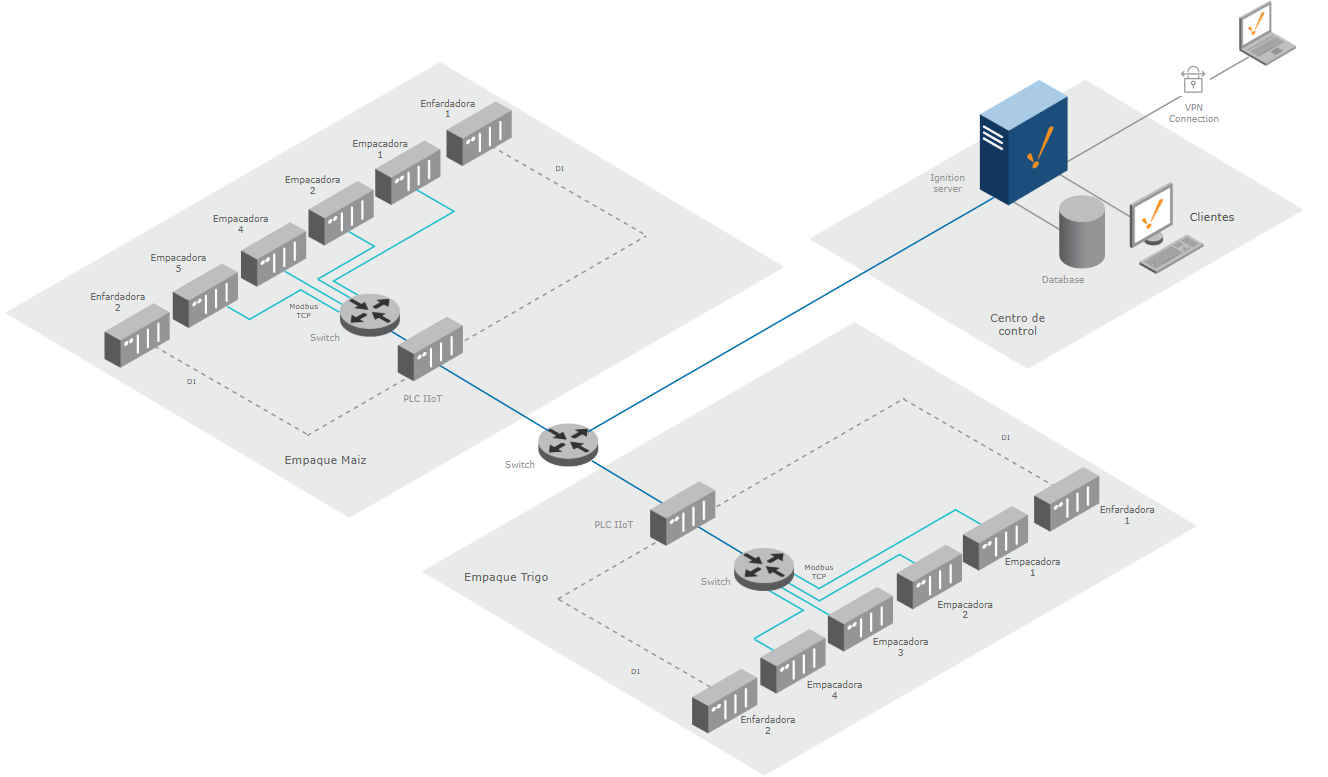
\includegraphics[width=1\textwidth]{Figuras/diagrama_arquitectura.png}
    \caption{Arquitectura IIoT del sistema de empaque integrado con UNS}
    \label{fig:arquitectura_iiot}
\end{figure}

\subsubsection{Componentes de la arquitectura}

La arquitectura IIoT implementada se compone de las siguientes capas y componentes:

\subsubsection{Capa de dispositivos de campo}

Esta capa incluye todos los controladores y señales que interactúan directamente con los procesos físicos de producción:

\begin{itemize}
    \item \textbf{PLCs Omron (8 unidades total):} 4 PLCs por área de empaque (1 por cada empacadora), encargados del control local y captura de variables de proceso.
    
    \item \textbf{Señales I/O de enfardadoras (4 unidades total):} 2 conjuntos de señales por área, que monitorizan el estado y conteo de las enfardadoras.
\end{itemize}

\subsubsection{Capa Edge/Gateway}

En esta capa se encuentran los PLCs Weidmüller que actúan como concentradores de datos (Data Gateways) para cada área de empaque:

\begin{itemize}
    \item \textbf{PLC Weidmüller - Área Empaque Trigo:} Recopila datos de las 4 empacadoras (PLCs Omron) y las 2 enfardadoras (señales I/O) del área de trigo.
    
    \item \textbf{PLC Weidmüller - Área Empaque Maíz:} Recopila datos de las 4 empacadoras (PLCs Omron) y las 2 enfardadoras (señales I/O) del área de maíz.
\end{itemize}

Las funciones principales de estos dispositivos incluyen:

\begin{itemize}
    \item Adquisición de datos desde PLCs Omron mediante protocolos industriales estándar
    \item Captura de señales I/O digitales de las enfardadoras
    \item Normalización y estructuración de datos en un formato unificado
    \item Comunicación con el centro de datos mediante protocolo OPC UA
    \item Buffering local de datos para garantizar entrega confiable ante fallas de red
\end{itemize}

\subsubsection{Capa de comunicación - OPC UA}

El protocolo OPC UA (Open Platform Communications Unified Architecture) se utiliza como medio de comunicación entre los PLCs Weidmüller y el centro de datos. Este protocolo industrial ofrece:

\begin{itemize}
    \item \textbf{Interoperabilidad:} Estándar abierto compatible con múltiples plataformas y fabricantes
    \item \textbf{Seguridad:} Cifrado de comunicaciones y autenticación de dispositivos
    \item \textbf{Orientación a objetos:} Modelado de información que facilita la organización jerárquica
\end{itemize}

\subsubsection{Capa UNS (Unified Namespace) - Centro de datos}

El núcleo de la arquitectura reside en el centro de datos, donde se implementa el Unified Namespace mediante la plataforma Ignition. Los componentes clave son:

\paragraph{Ignition Gateway}
Servidor central que:
\begin{itemize}
    \item Establece conexiones OPC UA con los PLCs Weidmüller de cada área
    \item Adquiere datos en tiempo real de todas las variables de proceso
    \item Aloja la aplicación MES (Manufacturing Execution System) para el agendamiento y gestión de órdenes de producción del área de empaque
\end{itemize}

La aplicación MES implementada en Ignition permite:
\begin{itemize}
    \item Crear y gestionar órdenes de producción para cada línea de empaque (Trigo y Maíz)
    \item Agendar la producción según demanda, disponibilidad de materia prima y capacidad de las líneas
    \item Asignar productos, cantidades objetivo y tiempos estimados a cada orden
    \item Hacer seguimiento en tiempo real del avance de cada orden de producción
    \item Registrar eventos de inicio, pausa y finalización de órdenes
    \item Asociar los datos de producción capturados (conteo de bolsas, tiempos, estados) con las órdenes activas
\end{itemize}

La integración entre el MES y los datos en tiempo real del UNS habilita el cálculo automático de KPIs operacionales, tales como:
\begin{itemize}
    \item \textbf{OEE (Overall Equipment Effectiveness):} Calculado a partir de la disponibilidad, rendimiento y calidad de cada empacadora en relación con las órdenes programadas
    \item \textbf{Cumplimiento de órdenes:} Porcentaje de órdenes completadas dentro del tiempo estimado
    \item \textbf{Eficiencia de línea:} Relación entre producción real y producción planificada por línea
    \item \textbf{Tiempo de ciclo promedio:} Promedio de tiempo requerido para empacar una unidad durante la orden
    \item \textbf{Tasa de producción:} Unidades producidas por hora en cada línea
    \item \textbf{Utilización de equipos:} Porcentaje del tiempo que cada empacadora estuvo activa durante el turno
\end{itemize}

Esta integración MES-UNS elimina la necesidad de captura manual de datos de producción y garantiza que todos los KPIs se basen en información confiable y en tiempo real.

\paragraph{Base de datos histórica}
Almacena series temporales de todas las variables para:
\begin{itemize}
    \item Análisis retrospectivo de producción
    \item Cumplimiento de requisitos de trazabilidad
\end{itemize}


\subsection{Estructura del namespace}

El namespace se estructura siguiendo una jerarquía basada en el estándar ISA-95, organizando los datos de forma lógica desde el nivel de empresa hasta el nivel de dispositivo individual. La estructura implementada para el caso de estudio es la siguiente:

\begin{verbatim}
Empresa/
└── Planta_Barranquilla/
    ├── Area_Empaque_Trigo/
    │   ├── Linea_1/
    │   │   ├── Empacadora_1/
    │   │   │   ├── Conteo_Bolsas
    │   │   │   ├── Tiempo_Ciclo
    │   │   │   ├── Estado_Maquina
    │   │   │   └── Eventos
    │   │   ├── Empacadora_2/
    │   │   │   ├── Conteo_Bolsas
    │   │   │   ├── Tiempo_Ciclo
    │   │   │   ├── Estado_Maquina
    │   │   │   └── Eventos
    │   │   └── Enfardadora/
    │   │       ├── Conteo_Bolsas_Entrada
    │   │       ├── Estado_Actividad
    │   │       └── Conteo_Fardos
    │   ├── Linea_2/
    │   │   ├── Empacadora_1/
    │   │   ├── Empacadora_2/
    │   │   └── Enfardadora/
    │   └── KPIs_Area/
    │       ├── Produccion_Total
    │       ├── OEE_Promedio
    │       └── Disponibilidad
    └── Area_Empaque_Maiz/
        ├── Linea_1/
        │   ├── Empacadora_1/
        │   ├── Empacadora_2/
        │   └── Enfardadora/
        ├── Linea_2/
        │   ├── Empacadora_1/
        │   ├── Empacadora_2/
        │   └── Enfardadora/
        └── KPIs_Area/
            ├── Produccion_Total
            ├── OEE_Promedio
            └── Disponibilidad
\end{verbatim}

\subsubsection{Niveles de la jerarquía}

La estructura del namespace sigue los siguientes niveles jerárquicos:

\paragraph{Nivel 1 - Empresa}
Nodo raíz que agrupa todas las instalaciones de la organización.

\paragraph{Nivel 2 - Planta/Sitio}
Identifica la ubicación física de la instalación (en este caso, Planta\_Barranquilla).

\paragraph{Nivel 3 - Área}
Agrupa los equipos por área funcional de producción:
\begin{itemize}
    \item Area\_Empaque\_Trigo
    \item Area\_Empaque\_Maiz
\end{itemize}

\paragraph{Nivel 4 - Línea de producción}
Cada área cuenta con dos líneas de producción independientes (Linea\_1, Linea\_2).

\paragraph{Nivel 5 - Equipo}
Identifica cada equipo individual dentro de la línea:
\begin{itemize}
    \item Empacadora\_1, Empacadora\_2 (por línea)
    \item Enfardadora (por línea)
\end{itemize}

\paragraph{Nivel 6 - Variables de proceso}
Tags individuales que contienen los valores de las variables monitorizadas.

\subsubsection{Ejemplo de rutas completas de tags}

A continuación se muestran ejemplos de rutas completas para algunos tags del sistema:

\begin{verbatim}
Empresa/Planta_Barranquilla/Area_Empaque_Trigo/Linea_1/
    Empacadora_1/Conteo_Bolsas

Empresa/Planta_Barranquilla/Area_Empaque_Maiz/Linea_2/
    Enfardadora/Estado_Actividad

Empresa/Planta_Barranquilla/Area_Empaque_Trigo/KPIs_Area/
    OEE_Promedio
\end{verbatim}

Esta nomenclatura garantiza que cualquier aplicación o usuario pueda identificar unívocamente la procedencia y significado de cada dato en el sistema.

\subsection{Requerimientos y desafíos de analítica de datos}

A partir de reuniones técnicas realizadas con el tutor designado por DAUTOM S.A.S., quien proporcionó acompañamiento especializado durante la caracterización del caso de estudio, se identificaron los requerimientos clave para la integración de una herramienta basada en LLM a la arquitectura UNS existente. Estas sesiones de trabajo permitieron comprender en profundidad las necesidades operacionales de la planta, los puntos críticos en la toma de decisiones y las limitaciones actuales en el acceso y análisis de información. 

A continuación se presentan los tres requerimientos principales identificados, junto con los desafíos técnicos asociados a cada uno de ellos. 

\subsubsection{Análisis detallado de requerimientos y desafíos}

A continuación se describe en detalle cada requerimiento identificado y los desafíos técnicos asociados a su implementación.

\paragraph{Requerimiento 1: Interpretación de consultas en lenguaje natural con conocimiento técnico del dominio}

\textbf{Descripción del requerimiento:}

El sistema LLM debe comprender consultas en lenguaje natural que incluyan términos técnicos de manufactura y ser capaz de identificar qué datos del UNS necesita consultar para responder. Esto implica que usuarios sin conocimientos técnicos profundos puedan realizar preguntas complejas sobre el proceso productivo y obtener respuestas precisas y contextualizadas.

\textbf{Desafíos identificados:}

\textit{D1.1 - Ambigüedad en términos técnicos:}

Palabras como "disponibilidad", "rendimiento" o "producción" pueden tener diferentes significados según el contexto en el que se utilicen. Por ejemplo, "disponibilidad" puede referirse a si la máquina está funcionando (uptime) o a si hay material disponible para producir. Similarmente, "rendimiento" puede aludir al rendimiento de una máquina individual (unidades producidas por hora) o al rendimiento global de una línea de producción.

El LLM debe entender el contexto de la pregunta para interpretar correctamente el término y acceder a las variables apropiadas del namespace. Esto requiere no solo procesamiento de lenguaje natural, sino también conocimiento del dominio industrial y la semántica de las métricas de manufactura.

\textit{D1.2 - Comprensión de relaciones entre variables:}

Preguntas como "¿por qué bajó la producción ayer?" requieren analizar múltiples factores que pueden estar relacionados: paros de máquinas no programados, incremento en tiempos de ciclo, cambios de producto que requieren ajustes, o falta de material en los silos. El LLM debe saber qué variables están relacionadas causalmente y buscar correlaciones entre ellas, no solo reportar un dato aislado.

Este desafío implica que el modelo debe tener capacidad de razonamiento sobre las relaciones funcionales entre diferentes componentes del sistema productivo y cómo estas interacciones afectan los KPIs resultantes.

\textit{D1.3 - Mapeo de lenguaje natural a la estructura del namespace:}

El usuario puede utilizar referencias ambiguas como "la empacadora de trigo" sin especificar cuál de las 4 empacadoras del área de trigo se está consultando. De manera similar, expresiones como "la línea A" pueden referirse a Línea A de Trigo o Línea A de Maíz.

El LLM debe ser capaz de pedir aclaraciones cuando sea necesario ("¿Te refieres a la Línea 1 del área de Trigo o de Maíz?") o usar el contexto previo de la conversación para resolver la ambigüedad de forma inteligente. Esto requiere mantener estado conversacional y aplicar heurísticas de resolución de referencias.

\paragraph{Requerimiento 2: Generación de reportes personalizados con análisis comparativos}

\textbf{Descripción del requerimiento:}

La herramienta debe generar reportes que no solo muestren números crudos, sino que incluyan comparaciones útiles (vs. día anterior, vs. otras líneas, vs. meta establecida en la orden de producción) y detecten automáticamente anomalías o patrones relevantes para la toma de decisiones.

\textbf{Desafíos identificados:}

\textit{D2.1 - Identificar qué comparaciones son relevantes:}

No todas las comparaciones tienen sentido o aportan valor en el contexto de manufactura. Por ejemplo, comparar la producción de un lunes con un domingo puede ser engañoso si los turnos de fin de semana operan con menor personal o producen referencias diferentes.

El LLM debe incorporar lógica operacional para saber qué comparaciones aportan valor en cada contexto. Esto incluye comparaciones con el mismo día de la semana anterior (para eliminar efectos de calendario), comparaciones entre líneas que producen el mismo producto (para identificar ineficiencias relativas), y comparaciones contra las metas establecidas en las órdenes de producción del MES.

\textit{D2.2 - Combinar datos de múltiples fuentes:}

Para generar reportes completos y contextualizados, el LLM debe integrar información de tres fuentes principales:

\begin{itemize}
    \item \textbf{UNS:} Datos operacionales en tiempo real (conteos actuales de bolsas, tiempos de ciclo recientes, estados actuales de máquinas, eventos de alarma activos).
    
    \item \textbf{MES integrado en Ignition:} Información contextual sobre la operación (qué orden de producción está activa, qué producto se está empacando, cantidades objetivo planificadas, tiempos programados de inicio y fin).
    
    \item \textbf{Base de datos histórica:} Datos de producción de días, semanas o meses anteriores que permiten análisis de tendencias, detección de degradación de equipos, y comparaciones temporales.
\end{itemize}

La integración coherente de estas fuentes permite que el LLM genere análisis completos. Por ejemplo: "La producción de hoy está 15\% por debajo del mismo día de la semana pasada (BD histórica), la Línea 1 está trabajando en la Orden \#12345 de harina de trigo presentación kilo con una meta de 5000 unidades (MES), y actualmente la Empacadora 2 está en estado de alarma desde hace 10 minutos (UNS), lo que explica la desviación observada".

Este desafío requiere que el LLM orqueste consultas a múltiples sistemas, reconcilie diferencias en granularidad temporal entre fuentes, y sintetice la información de forma coherente.

\textit{D2.3 - Adaptar el reporte según el perfil del usuario:}

Diferentes stakeholders en la organización tienen necesidades de información distintas:

\begin{itemize}
    \item Un \textbf{gerente de producción} necesita ver KPIs agregados por área, tendencias semanales o mensuales, y comparaciones de eficiencia entre turnos o líneas.
    
    \item Un \textbf{supervisor de turno} necesita detalles específicos sobre qué ocurrió durante su periodo de responsabilidad, en qué equipos se presentaron problemas, y qué acciones correctivas se tomaron.
    
    \item Un \textbf{técnico de mantenimiento} necesita información sobre frecuencia de fallas por equipo, tiempos promedio de reparación, y patrones de degradación que sugieran mantenimientos preventivos.
\end{itemize}

El sistema debe ser capaz de ajustar automáticamente el contenido, nivel de detalle, métricas presentadas y formato de salida según el perfil del usuario que realiza la consulta. Esto implica implementar perfiles de usuario con permisos y preferencias diferenciadas.

\paragraph{Requerimiento 3: Acceso eficiente a datos históricos y en tiempo real}

\textbf{Descripción del requerimiento:}

El sistema debe poder consultar tanto los datos en tiempo real disponibles en el UNS como el histórico almacenado en bases de datos relacionales, y combinarlos de forma coherente para responder consultas que abarquen diferentes periodos de tiempo, desde minutos recientes hasta meses o años anteriores.

\textbf{Desafíos identificados:}

\textit{D3.1 - Generar consultas eficientes a la base de datos:}

El LLM debe traducir preguntas en lenguaje natural a consultas de base de datos (SQL) que sean eficientes y no generen carga computacional excesiva. Por ejemplo, si el usuario pregunta "¿cuál fue el promedio de producción del último mes?", el LLM debe generar una query que utilice tablas agregadas pre-calculadas o índices apropiados, en lugar de escanear millones de registros individuales.

Esto requiere que el LLM tenga conocimiento de:
\begin{itemize}
    \item El esquema de la base de datos (tablas, columnas, relaciones)
    \item Los índices disponibles y cómo aprovecharlos
    \item Estrategias de agregación eficiente (uso de tablas materializadas, vistas agregadas)
    \item Limitaciones de rendimiento del sistema de base de datos
\end{itemize}

La generación de queries SQL eficientes es crítica para garantizar tiempos de respuesta aceptables, especialmente cuando se consultan periodos extensos con alta densidad de datos.

\textit{D3.2 - Seleccionar la granularidad adecuada de los datos:}

Los datos industriales se almacenan con diferentes frecuencias de muestreo dependiendo de la variable y el propósito. Para periodos cortos de tiempo (última hora, último turno) es apropiado usar datos de alta frecuencia que capturan cada evento significativo. Sin embargo, para periodos largos (último mes, último trimestre) es más eficiente usar agregaciones por hora, por turno, o por día.

El LLM debe decidir automáticamente qué nivel de detalle (granularidad) usar según el rango temporal que especifica el usuario en su consulta. Por ejemplo:
\begin{itemize}
    \item "Producción en los últimos 30 minutos" → datos con granularidad de minutos
    \item "Producción del día de ayer" → datos agregados por hora
    \item "Producción del último mes" → datos agregados por día o por turno
\end{itemize}

Esta selección automática de granularidad balancea la precisión de la respuesta con la eficiencia computacional, evitando procesar datos innecesariamente detallados cuando no aportan valor adicional a la consulta.

\subsubsection{Síntesis de requerimientos y desafíos}

Los tres requerimientos identificados y sus desafíos asociados representan los aspectos técnicos críticos que debe abordar la integración de una herramienta LLM con la arquitectura UNS del caso de estudio. El Requerimiento 1 se enfoca en las capacidades de comprensión del lenguaje natural y mapeo al dominio industrial. El Requerimiento 2 aborda la generación inteligente de insights y la personalización de reportes. El Requerimiento 3 trata los aspectos de arquitectura de datos y eficiencia en el acceso a información histórica y en tiempo real.

Estos requerimientos guiarán el diseño de la solución propuesta en los capítulos subsiguientes y servirán como base para la definición de métricas de validación del sistema integrado.





\cleardoublepage

\section{Capitulo 3: Selección del mecanismo de integración y herramienta LLM}
\label{seleccionllm}

Con la arquitectura UNS implementada (Capítulo 2), el siguiente paso consiste en definir cómo se conecta un modelo de lenguaje de gran tamaño (LLM) a esa estructura de datos. Esta decisión tiene dos partes: primero, qué mecanismo de comunicación usar entre el UNS y el LLM; segundo, qué herramienta LLM emplear. Este capítulo desarrolla ambos aspectos, siguiendo el análisis comparativo documentado que exige la propuesta de este trabajo.

\subsection{Mecanismos de integración de LLM con sistemas externos en IIoT}
\label{mecanismosintegracion}

Conectar un LLM a una fuente de datos externa no es un problema nuevo, pero sí lo es hacerlo en un contexto industrial donde la fuente cambia constantemente de valor y donde una mala configuración puede exponer información sensible del proceso. La literatura y la práctica de la industria coinciden en tres formas de resolver esta conexión: invocación directa mediante HTTP/REST, orquestación mediante pipelines de procesamiento, y Model Context Protocol (MCP) \cite{MastouriRESTtoMCP2026, EhteshamAgentProtocols2025}. Las tres se describen a continuación de forma general, antes de compararlas frente al caso de estudio en la Sección \ref{analisiscomparativo}.

\subsubsection{Invocación directa mediante HTTP/REST}

REST (\textit{Representational State Transfer}) es un estilo arquitectónico para sistemas distribuidos, no un protocolo en sí mismo \cite{ReSTFielding2000}. Se apoya sobre HTTP y define un conjunto de restricciones: interfaz uniforme, recursos identificables mediante URI, y comunicación sin estado, donde cada petición contiene toda la información necesaria para procesarla, sin depender de peticiones anteriores.

Aplicado a la integración de un LLM con una fuente de datos industrial, este enfoque implica exponer los datos del UNS como un conjunto de \textit{endpoints} (por ejemplo, \texttt{GET /linea/A/oee}), que el LLM invoca mediante peticiones HTTP explícitas. El desarrollador debe programar de antemano cuál endpoint corresponde a determinada consulta, ya que el LLM no tiene forma nativa de descubrir en tiempo de ejecución qué recursos existen ni qué significan. Cada nueva fuente de datos (una línea adicional, un nuevo sistema ERP) exige escribir y mantener el conector correspondiente. Este patrón de integración ad hoc, repetido por cada combinación de modelo y fuente de datos, es lo que en la industria se conoce como el problema de los conectores fragmentados \cite{anthropic2024intro}.

\subsubsection{Orquestación mediante pipelines de procesamiento}

Un segundo enfoque introduce una capa intermedia entre el LLM y las fuentes de datos: un motor de orquestación que define, paso a paso, cómo se recupera, transforma y entrega la información al modelo. A diferencia de la invocación directa, aquí el LLM no llama a la fuente de datos por sí mismo; el pipeline decide qué pasos ejecutar, en qué orden y con qué transformaciones intermedias, y solo entrega al LLM el resultado ya procesado.

Este patrón es común en frameworks de orquestación de agentes, donde cada paso del pipeline puede invocar una API distinta, aplicar una regla de negocio o enriquecer el dato con contexto adicional antes del siguiente paso \cite{EhteshamAgentProtocols2025}. La ventaja operativa se tiene el control explícito sobre el flujo de datos, mientras que como desventaja se tiene que el control depende enteramente de cómo se configuró el pipeline: agregar una nueva fuente o un nuevo tipo de consulta no es tan simple como registrar un endpoint, sino que exige modificar la lógica del pipeline mismo.

\subsubsection{Model Context Protocol (MCP)}

MCP es un estándar abierto introducido por Anthropic a finales de 2024, diseñado para conectar asistentes de IA con las fuentes de datos y herramientas externas donde reside la información \cite{anthropic2024intro}. A diferencia de los dos mecanismos anteriores, MCP no fue diseñado pensando en un desarrollador que programa una integración, sino en un modelo de lenguaje que necesita descubrir, en tiempo de ejecución, qué herramientas y datos tiene disponibles.

Su arquitectura sigue un modelo cliente-servidor: una aplicación de IA actúa como anfitrión MCP y se conecta a uno o más servidores MCP mediante clientes dedicados, cada uno con una conexión independiente \cite{anthropic2024arch}. La comunicación se organiza en dos capas: una capa de datos basada en JSON-RPC 2.0, que define la negociación de capacidades y la exposición de funcionalidades del servidor, y una capa de transporte que gestiona la conexión y la autenticación, ya sea local (STDIO) o remota (HTTP, con soporte para OAuth) \cite{anthropic2024arch}.

El concepto central son las primitivas de contexto que el servidor expone al cliente: \textit{Tools} (funciones ejecutables, como consultar un tag o disparar una acción), \textit{Resources} (fuentes de datos con contexto estructurado) y \textit{Prompts} (plantillas reutilizables) \cite{anthropic2024arch}. Sobre esta base, MCP también incorpora un sistema de notificaciones al que el cliente puede suscribirse para mantenerse sincronizado con cambios en el servidor, evitando así las consultas repetidas propias de otros mecanismos.

% TODO-FIGURA 1
\begin{figure}[H]
\centering
 \centerline{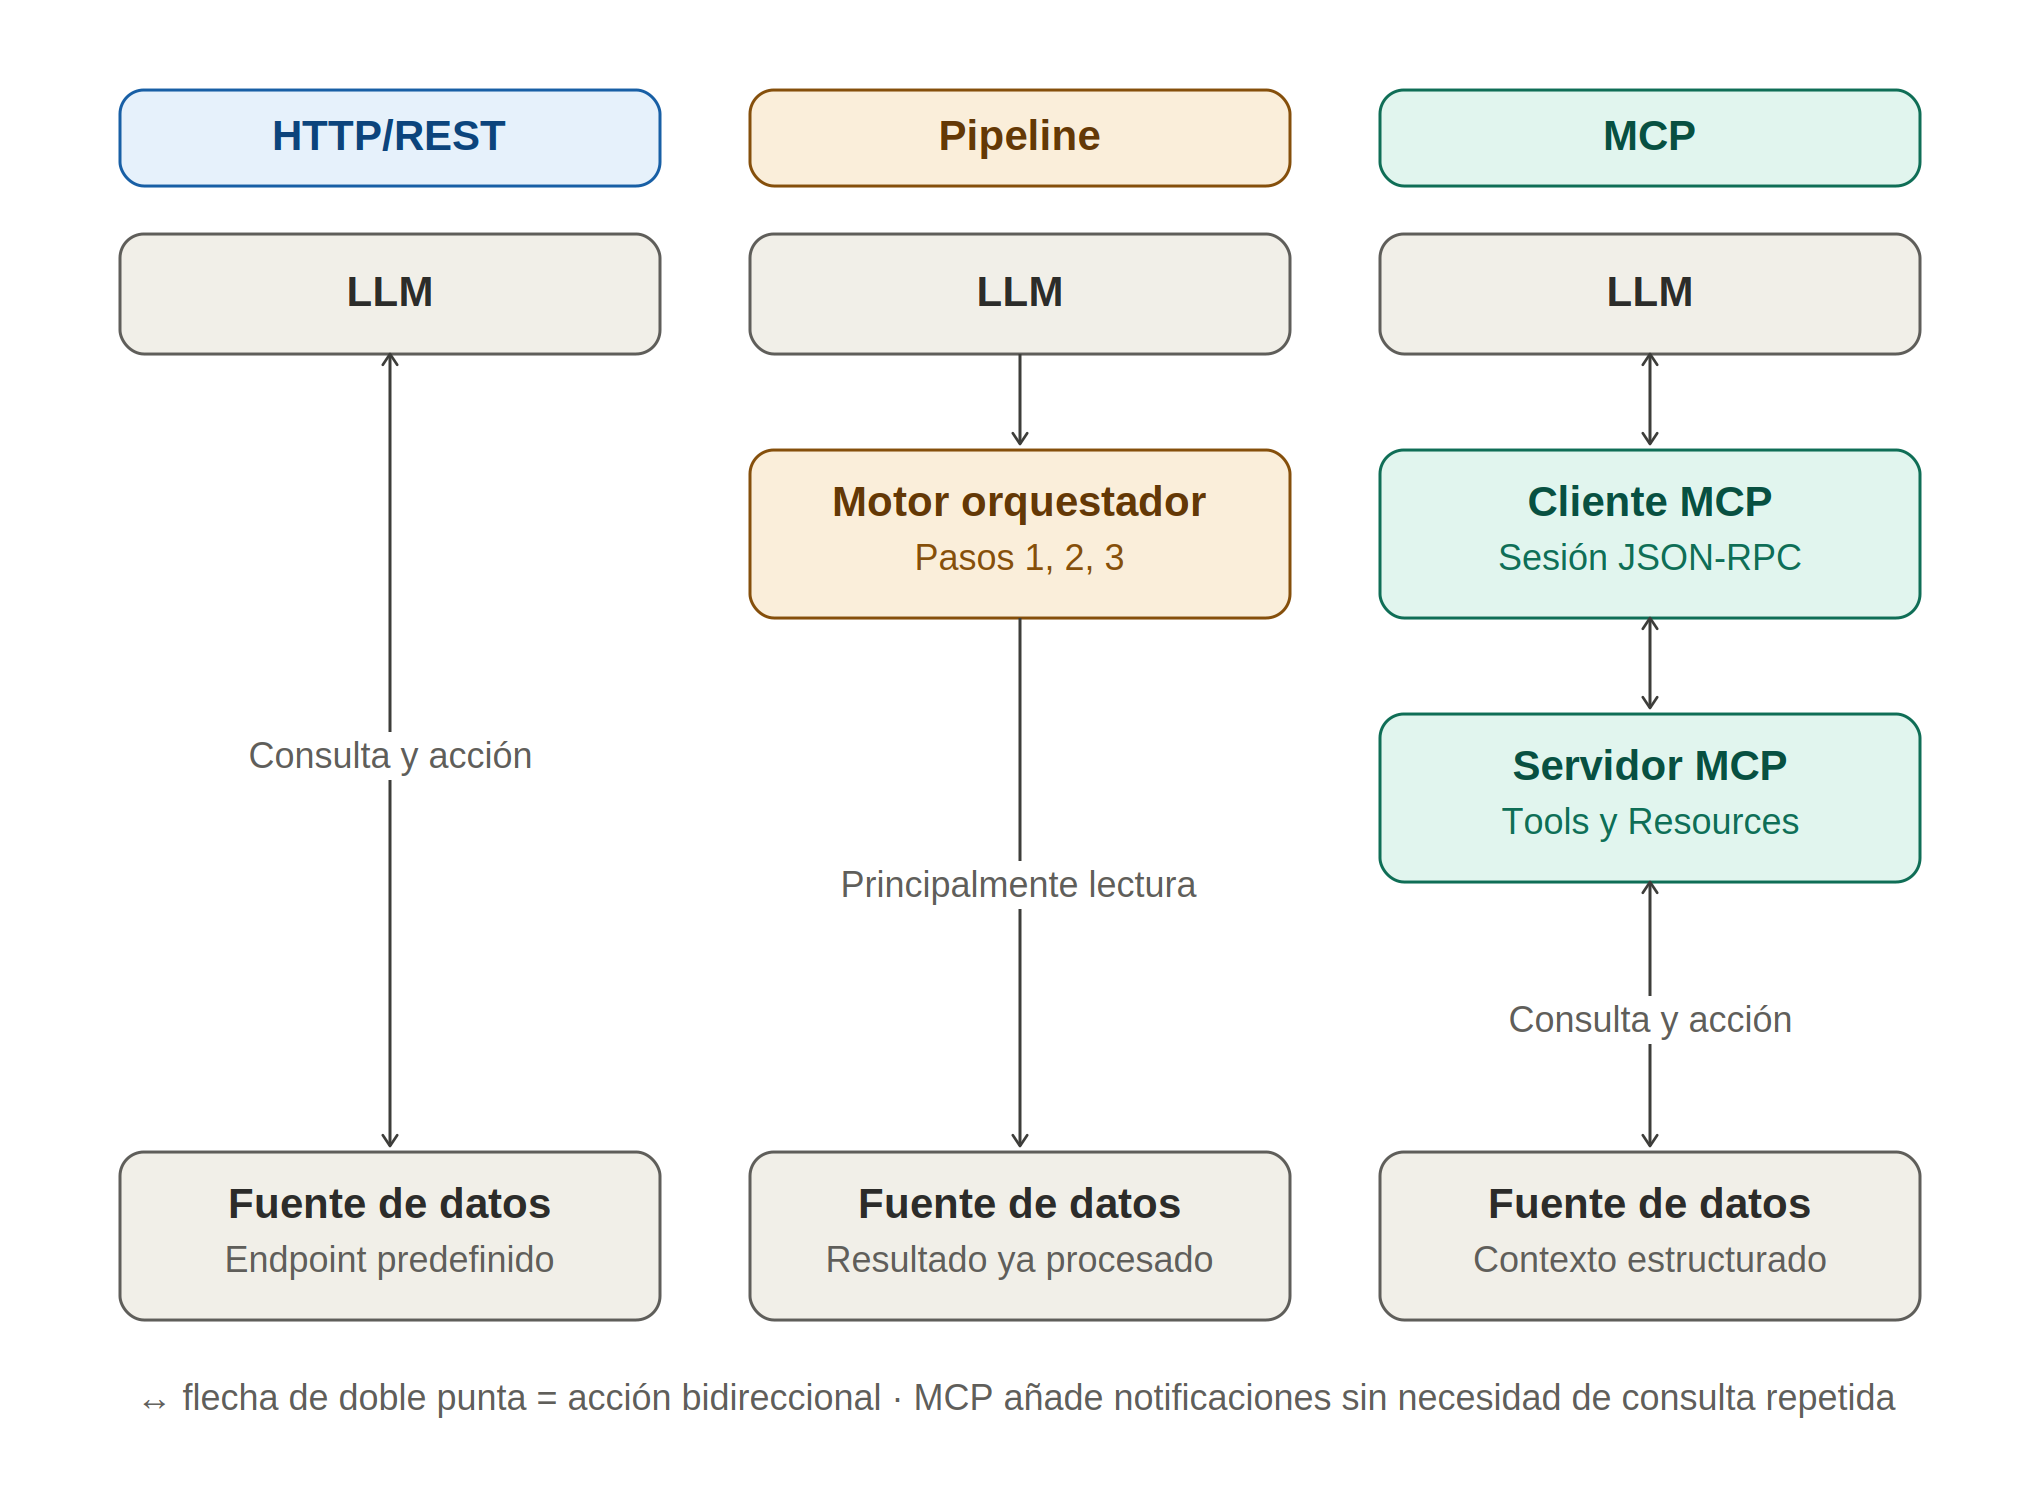
\includegraphics[width=13cm]{Figuras/mecanismos_integracion.png}}
\caption{Comparación esquemática de los mecanismos de integración LLM-UNS: HTTP/REST, pipeline de orquestación y MCP. Elaboración propia.}
\label{fig:mecanismos_integracion}
\end{figure}


\subsection{Criterios de comparación}
\label{criterioscomparacion}

Comparar estos tres mecanismos exige criterios concretos, no una preferencia general por lo más reciente o lo más popular. Se definieron seis criterios, anclados a tres fuentes distintas: los tres primeros provienen textualmente de la justificación de la propuesta de este trabajo; el cuarto y el quinto se derivan de los requerimientos funcionales identificados en la caracterización del caso de estudio (Capítulo 1, R1 y R2/R3); el sexto es un criterio técnico complementario, sin anclaje directo en la propuesta, incluido por buenas prácticas de arquitectura de software.

\begin{enumerate}
    \item \textbf{Acceso a variables en tiempo real} (propuesta). Mide si el mecanismo permite consultar el estado actual del proceso sin latencia significativa ni pasos intermedios de sincronización.
    \item \textbf{Acción bidireccional} (propuesta). Mide si el mecanismo permite no solo leer datos del UNS, sino también escribir o ejecutar acciones sobre el sistema.
    \item \textbf{Restricciones de privacidad IIoT} (propuesta). Mide la granularidad del control de acceso y la madurez de los mecanismos de autenticación y autorización propios del mecanismo.
    \item \textbf{Capacidad de exponer contexto semántico} (R1). Mide si el mecanismo transmite al LLM el significado del dato (jerarquía, unidades, procedencia), no solo su valor crudo.
    \item \textbf{Esfuerzo de desarrollo y mantenimiento} (R2/R3). Mide cuánto código a la medida hay que escribir y sostener para conectar cada fuente de datos del UNS.
    \item \textbf{Interoperabilidad multi-proveedor} (técnico). Mide el grado de acoplamiento de la solución a un único proveedor de LLM.
\end{enumerate}

\subsection{Análisis comparativo de los mecanismos de integración}
\label{analisiscomparativo}

La Tabla \ref{tab:comparacion_mecanismos} resume la evaluación de los tres mecanismos frente a los seis criterios definidos. La calificación usa tres niveles: \checkmark\checkmark~(cumple de forma robusta), \checkmark~(cumple de forma parcial o requiere trabajo adicional) y \texttimes~(no cumple o presenta una limitación significativa).

\begin{table}[H]
\centering
\caption{Comparación de mecanismos de integración LLM-UNS frente a los seis criterios definidos.}
\label{tab:comparacion_mecanismos}
\begin{tabular}{p{4.3cm}ccc}
\hline
\textbf{Criterio} & \textbf{HTTP/REST} & \textbf{Pipelines} & \textbf{MCP} \\
\hline
Acceso en tiempo real & \checkmark & \texttimes & \checkmark\checkmark \\
Acción bidireccional & \checkmark & \texttimes & \checkmark\checkmark \\
Privacidad IIoT & \checkmark\checkmark & \checkmark & \texttimes \\
Contexto semántico & \texttimes & \checkmark & \checkmark\checkmark \\
Esfuerzo de desarrollo & \texttimes & \texttimes & \checkmark\checkmark \\
Interoperabilidad multi-proveedor & \checkmark & \texttimes & \checkmark\checkmark \\
\hline
\end{tabular}
\end{table}

\textbf{Acceso a variables en tiempo real.} HTTP/REST permite lectura bajo demanda, pero depende de que el cliente pregunte (\textit{polling}); no hay un mecanismo nativo para que el servidor avise de un cambio. Los pipelines de orquestación añaden latencia adicional por las etapas intermedias de procesamiento, lo que los deja en la posición más débil de los tres. MCP resuelve esto mediante suscripción, su sistema de notificaciones mantiene al cliente sincronizado sin necesidad de consultas repetidas \cite{anthropic2024arch}, lo que se traduce en acceso inmediato al estado del proceso, tal como demuestran Yang et al. en su implementación de MCP sobre sistemas IoT industriales \cite{YangIoTMCP2025}.

\textbf{Acción bidireccional.} REST soporta lectura y escritura a nivel de protocolo (GET, POST, PUT), pero el LLM necesita saber de antemano cuál endpoint invocar para cada acción, sin mecanismo de descubrimiento. Los pipelines suelen diseñarse para flujos de lectura y transformación; añadir escritura implica construir pasos adicionales de forma explícita. MCP fue diseñado desde el inicio para conexiones bidireccionales entre la aplicación de IA y las fuentes externas \cite{anthropic2024intro}, con la ventaja adicional de que la acción queda descrita junto con su contexto semántico dentro del bloque primitivo \textit{Tool}.

\textbf{Restricciones de privacidad IIoT.} Este es el único criterio donde REST aventaja claramente a los otros dos. Sus mecanismos de autenticación y autorización (OAuth2, API keys) son robustos y han sido ampliamente usados en auditoría en producción. MCP, al ser una tecnología emergente, presenta una superficie de ataque documentada: Hou et al. identifican dieciséis escenarios de amenaza distribuidos en las cuatro fases del ciclo de vida de un servidor MCP, incluyendo envenenamiento de herramientas y ejecución remota no autorizada \cite{HouMCPLandscape2025}. Los pipelines de orquestación quedan en una posición intermedia: su seguridad depende enteramente de cómo se implementó el motor de orquestación, sin un estándar unificado que la respalde.

\textbf{Capacidad de exponer contexto semántico.} La respuesta de un endpoint REST es, por diseño, un valor sin contexto adicional; el significado de ese valor vive en la documentación externa que el LLM no consulta durante la ejecución. Un pipeline puede enriquecer el dato en sus etapas intermedias, pero solo si alguien diseñó esa etapa explícitamente. El bloque primitivo \textit{Resources} de MCP resuelve este problema de forma estructural, al exponer no solo el dato sino su procedencia dentro de la jerarquía del servidor \cite{anthropic2024arch}. La revisión sistemática de Abu-Salih et al. sobre el uso de LLM para interoperabilidad semántica confirma que este tipo de exposición estructurada de contexto es, hasta ahora, el factor que más impacta la calidad de las respuestas de un LLM sobre datos heterogéneos \cite{AbuSalihSemanticLLM2025}.

\textbf{Esfuerzo de desarrollo y mantenimiento.} REST exige un conector a la medida por cada fuente de datos del UNS; los pipelines suman a ese esfuerzo el mantenimiento del propio motor de orquestación, lo que los ubica como la opción más costosa de sostener en el tiempo. MCP invierte esta lógica: en lugar de construir un conector por combinación de modelo y fuente, se construye un servidor MCP una sola vez, reutilizable por cualquier cliente compatible \cite{AhmadiMCPBridge2025}. El estudio presentado por Chen et al., basado en entrevistas con veinte profesionales de ocho empresas, confirma que la reducción de conectores a la medida es, en la práctica, el beneficio que más valoran los equipos que adoptan MCP en flujos de trabajo con LLM \cite{ChenEnterpriseMCP2026}.

\textbf{Interoperabilidad multi-proveedor.} REST es neutral por diseño: cualquier LLM puede invocar un endpoint REST si se le programa la lógica correspondiente, aunque esa lógica deba reescribirse para cada proveedor. Los pipelines suelen depender del framework de orquestación elegido, lo que introduce un acoplamiento adicional no siempre compatible con distintos proveedores de LLM. MCP, al ser un estándar abierto, ha sido adoptado como protocolo de host por múltiples proveedores más allá de Anthropic \cite{EhteshamAgentProtocols2025}, lo que reduce el riesgo de atar la arquitectura del caso de estudio a una única herramienta LLM.

El balance final es de cinco criterios a favor de MCP y uno a favor de HTTP/REST. Vale la pena señalar que este resultado no oculta una limitación real de MCP: el criterio donde pierde, privacidad, no es menor en un contexto industrial, y se retoma en la sección siguiente como parte de la decisión, no como una nota al margen.

\subsection{Selección del mecanismo de integración}
\label{seleccionmecanismo}

Con base en el análisis de la Sección \ref{analisiscomparativo}, se selecciona MCP como mecanismo de integración entre el LLM y la arquitectura UNS del caso de estudio. La decisión se apoya en que las prioridades del caso de estudio (acceso a datos de producción en tiempo real, capacidad de que el LLM actúe sobre el sistema, y necesidad de exponer contexto semántico de una jerarquía de datos compleja) coinciden exactamente con los criterios donde MCP demostró ventaja.

La brecha en privacidad no se ignora. Dado que MCP aún no iguala la madurez de REST en control de acceso, esta limitación se reconoce como un riesgo aceptado en esta fase de selección del mecanismo, que deberá abordarse durante la implementación de la integración sobre el caso de estudio (Capítulo 4), en vez de resolverse aquí con una medida que el análisis comparativo no sustentó.

Como referencia para esa implementación, tres decisiones de diseño concretas pueden reducir esa brecha sin necesidad de mecanismos ajenos al protocolo: adoptar transporte STDIO en lugar de HTTP remoto, dado que el servidor Ignition del caso de estudio es local y no requiere exposición de red; limitar el alcance del servidor MCP a herramientas de lectura sobre los contextos MES, Line, ERP y Edge ya definidos en el Capítulo 2, sin incluir operaciones de escritura ni acceso a la configuración interna de Ignition; y, si en el futuro se requiere un transporte remoto, exigir autenticación OAuth en esa capa, tal como lo contempla la especificación del protocolo \cite{anthropic2024arch}.

% TODO-FIGURA 2
\begin{figure}[H]
\centering
 \centerline{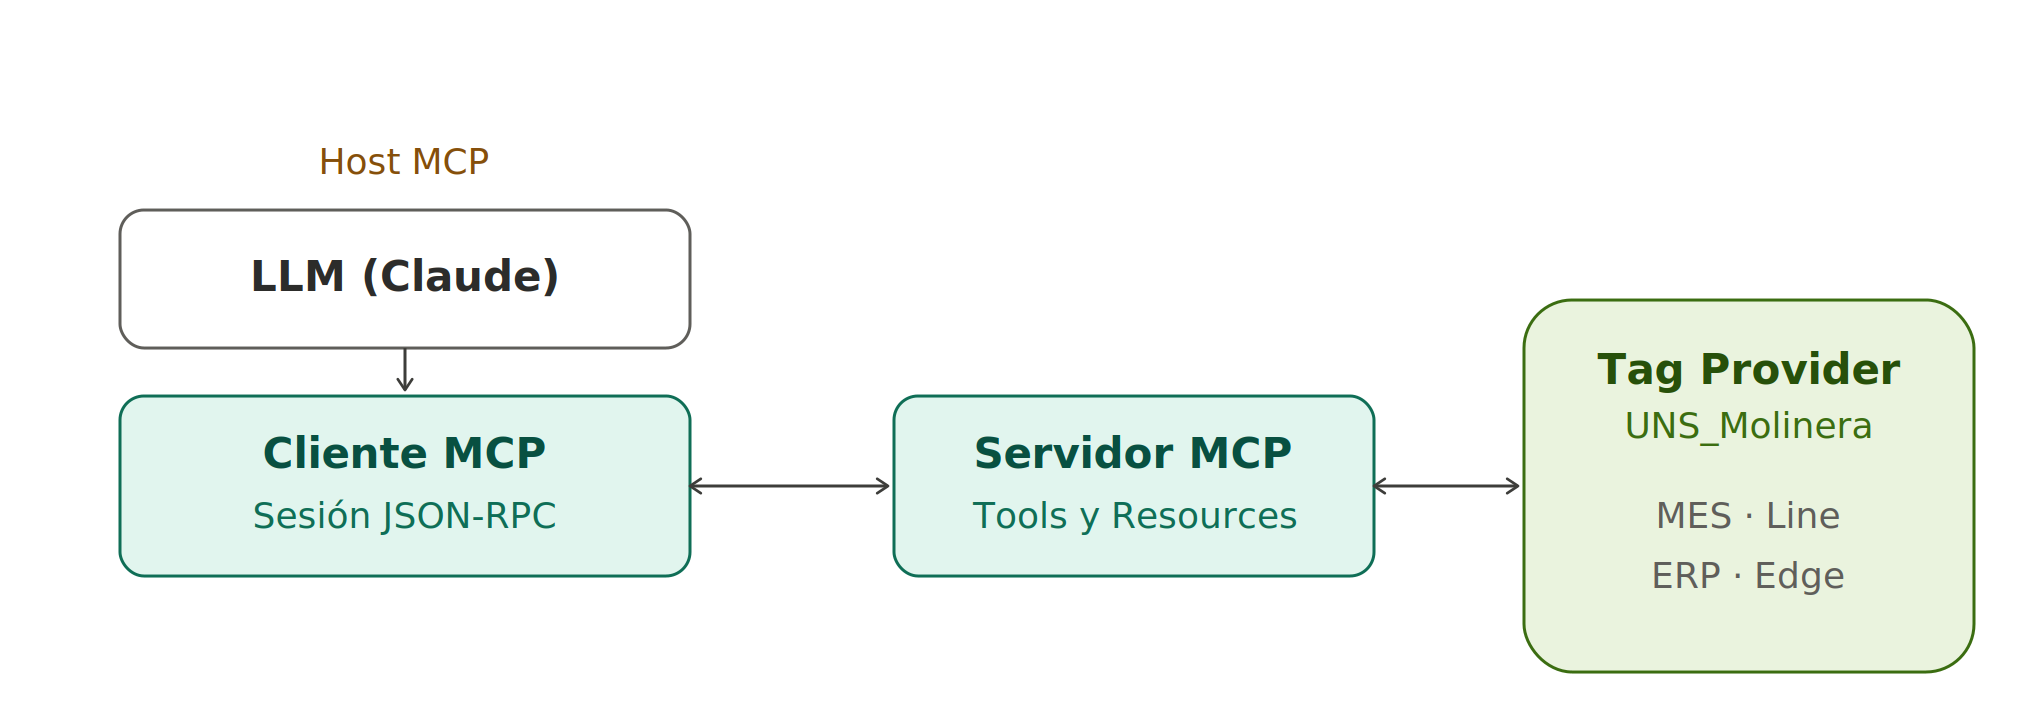
\includegraphics[width=15cm]{Figuras/mcp_uns.png}}
\caption{Arquitectura de integración seleccionada: servidor MCP entre el LLM y el Tag Provider \texttt{UNS\_Molinera}. Elaboración propia.}
\label{fig:mcp_lista_blanca}
\end{figure}

La Figura \ref{fig:mcp_lista_blanca} resume el flujo de una consulta típica. Cuando el LLM necesita un dato, el Cliente MCP invoca al Servidor MCP a través de la conexión establecida, especificando la herramienta y los parámetros correspondientes. El Servidor MCP traduce esa invocación en una lectura sobre el Tag Provider \texttt{UNS\_Molinera}, y devuelve el resultado ya estructurado con su contexto (a qué línea, a qué corrida y a qué unidad de medida corresponde), no solo el valor crudo. Cuando una pregunta requiere combinar más de un contexto de datos (por ejemplo, cruzar el contexto ERP con el MES para responder si una línea va atrasada respecto a su meta), este ciclo de invocación y respuesta se repite tantas veces como sea necesario antes de que el LLM redacte la respuesta final, sin que el operador tenga que descomponer la pregunta en pasos.

\subsection{Selección de la herramienta LLM}
\label{seleccionherramientallm}

\subsubsection{Criterios de adaptabilidad al caso de estudio}

Definido el mecanismo de integración, la elección de la herramienta LLM se evalúa contra tres criterios de adaptabilidad al caso de estudio, distintos de los seis usados para comparar mecanismos, porque aquí la pregunta ya no es qué protocolo usar sino qué modelo aprovecha mejor ese protocolo.

El primero es el soporte nativo del protocolo MCP como anfitrión (\textit{host}), sin requerir adaptadores intermedios que traduzcan entre el modelo y el servidor MCP. El segundo es la capacidad de razonamiento necesaria para encadenar múltiples invocaciones de herramientas y sintetizar resultados de distintas fuentes en una sola respuesta coherente, capacidad que la literatura sobre agentes basados en LLM describe como el patrón de intercalar razonamiento y acción en pasos sucesivos \cite{YaoReAct2023}. El tercero es la capacidad de interpretar y mapear terminología técnica del dominio industrial a las variables correspondientes de la jerarquía UNS, de modo que una pregunta formulada en lenguaje natural por un operador se traduzca correctamente en la ruta de tags adecuada.

\subsubsection{Selección de Claude (Anthropic)}

Se selecciona Claude (Anthropic) como herramienta LLM para este trabajo. La justificación sigue los tres criterios anteriores.

Sobre soporte nativo de MCP, Claude fue el primer anfitrión de referencia del protocolo, dado que Anthropic es su creador y mantiene la especificación oficial \cite{anthropic2024arch}; esto elimina la necesidad de un adaptador intermedio entre el modelo y el servidor MCP construido para el caso de estudio.

Sobre capacidad de razonamiento para encadenar herramientas, Claude sostiene conversaciones donde una sola consulta del operador puede requerir varias invocaciones sucesivas al servidor MCP (por ejemplo, leer el estado de la línea, cruzarlo con la orden de producción activa, y solo entonces responder), sin que el operador tenga que descomponer la pregunta en pasos. Esta capacidad corresponde al patrón de razonamiento y acción intercalados que Yao et al. formalizaron como ReAct \cite{YaoReAct2023}, y que en el caso de estudio se traduce en preguntas como "¿vamos atrasados respecto a la meta?", que exige combinar datos del contexto ERP con el contexto MES en una sola respuesta.

Sobre mapeo de terminología técnica del dominio, la jerarquía UNS de este trabajo usa nombres de tags en inglés técnico (\texttt{OEE}, \texttt{Infeed}, \texttt{RunID}) mientras que los operadores de planta consultan en español y con vocabulario propio de la industria de molienda. Esta traducción entre lenguaje natural del dominio y variables estructuradas es precisamente el tipo de tarea que estudios recientes de integración de LLM en entornos de manufactura han evaluado con resultados favorables cuando el modelo tiene acceso a herramientas con contexto semántico explícito \cite{AbuSalihSemanticLLM2025}, condición que ya se cumple gracias a la primitiva \textit{Resources} de MCP descrita en la Sección \ref{mecanismosintegracion}.

\subsection{Síntesis del capítulo}

Este capítulo resolvió las dos preguntas planteadas al inicio: qué mecanismo usar para conectar un LLM a la arquitectura UNS, y qué herramienta LLM emplear. El análisis comparativo, sustentado en seis criterios anclados a la propuesta, a los requerimientos del caso de estudio y a buenas prácticas técnicas, llevó a seleccionar MCP como mecanismo de integración, reconociendo su brecha en privacidad frente a REST y dejando como lineamiento para la fase de implementación un conjunto de decisiones de diseño concretas (transporte STDIO, alcance mínimo del servidor, autenticación OAuth para escenarios remotos) que la reducen sin recurrir a mecanismos ajenos al protocolo. Sobre esa base, se seleccionó Claude como herramienta LLM, justificada en su soporte nativo del protocolo, su capacidad de razonamiento para encadenar herramientas y su aptitud para mapear terminología técnica del dominio industrial. El siguiente capítulo documenta cómo se implementó esta integración sobre la arquitectura UNS del caso de estudio.
\cleardoublepage



\section{Capitulo 4: Implementación de Técnicas UNS en la Plataforma IIoT}
La implementación del UNS en la plataforma de entrenamiento IIoT se basa en la aplicación de técnicas de diseño previamente estudiadas en un entorno académico. Esta aplicación integra sistemas y dispositivos mediante el protocolo MQTT Sparkplug B, estableciendo un modelo jerárquico y estructurado de comunicación orientado a la gestión eficiente de datos.

Este entorno de entrenamiento simula escenarios operacionales reales de la industria  permitiendo a los usuarios interactuar directamente con dispositivos IIoT y validar los principios del UNS en tiempo real.


\subsection{Descripción de la Plataforma IIoT}
La construcción de la plataforma IIoT para entrenamiento en tecnologías de la Industria 4.0 surge como resultado de dos proyectos de investigación estratégicos. El primero, desarrollado bajo la Convocatoria interna VIE en 2021, llevó por título "Plataforma IIoT para formación de profesionales en tecnologías de la cuarta revolución industrial" y se ejecutó entre noviembre de 2021 y noviembre de 2023. Posteriormente, el proyecto "Diseño, desarrollo e implementación de una plataforma IIoT para formación de profesionales en tecnologías de la cuarta revolución industrial", financiado por la Convocatoria 890 de Minciencias, inició en abril de 2023 y se encuentra actualmente en desarrollo. 


\subsubsection{Dispositivos y Nodos Industriales:}
La plataforma se compone de tres casos de estudio, cada uno asociado a un grupo de investigación y con aplicaciones específicas en entornos industriales y académicos:


\begin{itemize}
    \item \textbf{VIVERO:} Pertenece al Grupo de Investigación CENIVAM, donde se monitorean condiciones ambientales dentro de un invernadero mediante un PLC Opto22 - Groov RIO conectado a un termohigrómetro que captura datos de temperatura y humedad. Estos datos son procesados por un servidor Ignition Edge para ser transmitidos.

    \item \textbf{CASIRI:} Pertenece a los Grupos de Investigación RADIOGIS y CEMOS, consiste en una estación de radioastronomía equipada con sensores ambientales que miden temperatura, humedad, presión atmosférica, velocidad y dirección del viento; además de  una cámara multi-espectral para captura de imágenes espectrales y un dispositivo de monitoreo del espectro radioeléctrico. Todos estos dispositivos están integrados mediante un servidor que envía los datos al servidor central.

    \item \textbf{MICRORRED:} Pertenece al Grupo de Investigación GISEL, ubicada en el Laboratorio de Investigación Eléctrica (LIE) en la sede UIS Guatiguara. Este sistema monitorea parámetros críticos de la red eléctrica como tensión RMS, corriente RMS, factor de potencia y diferentes tipos de potencia (aparente, activa y reactiva) mediante un PLC Opto22 - Groov EPIC que utiliza un servidor de Ignition Edge para  prestar servicios a los usuarios.

\end{itemize}

\begin{figure}[h]
\centerline{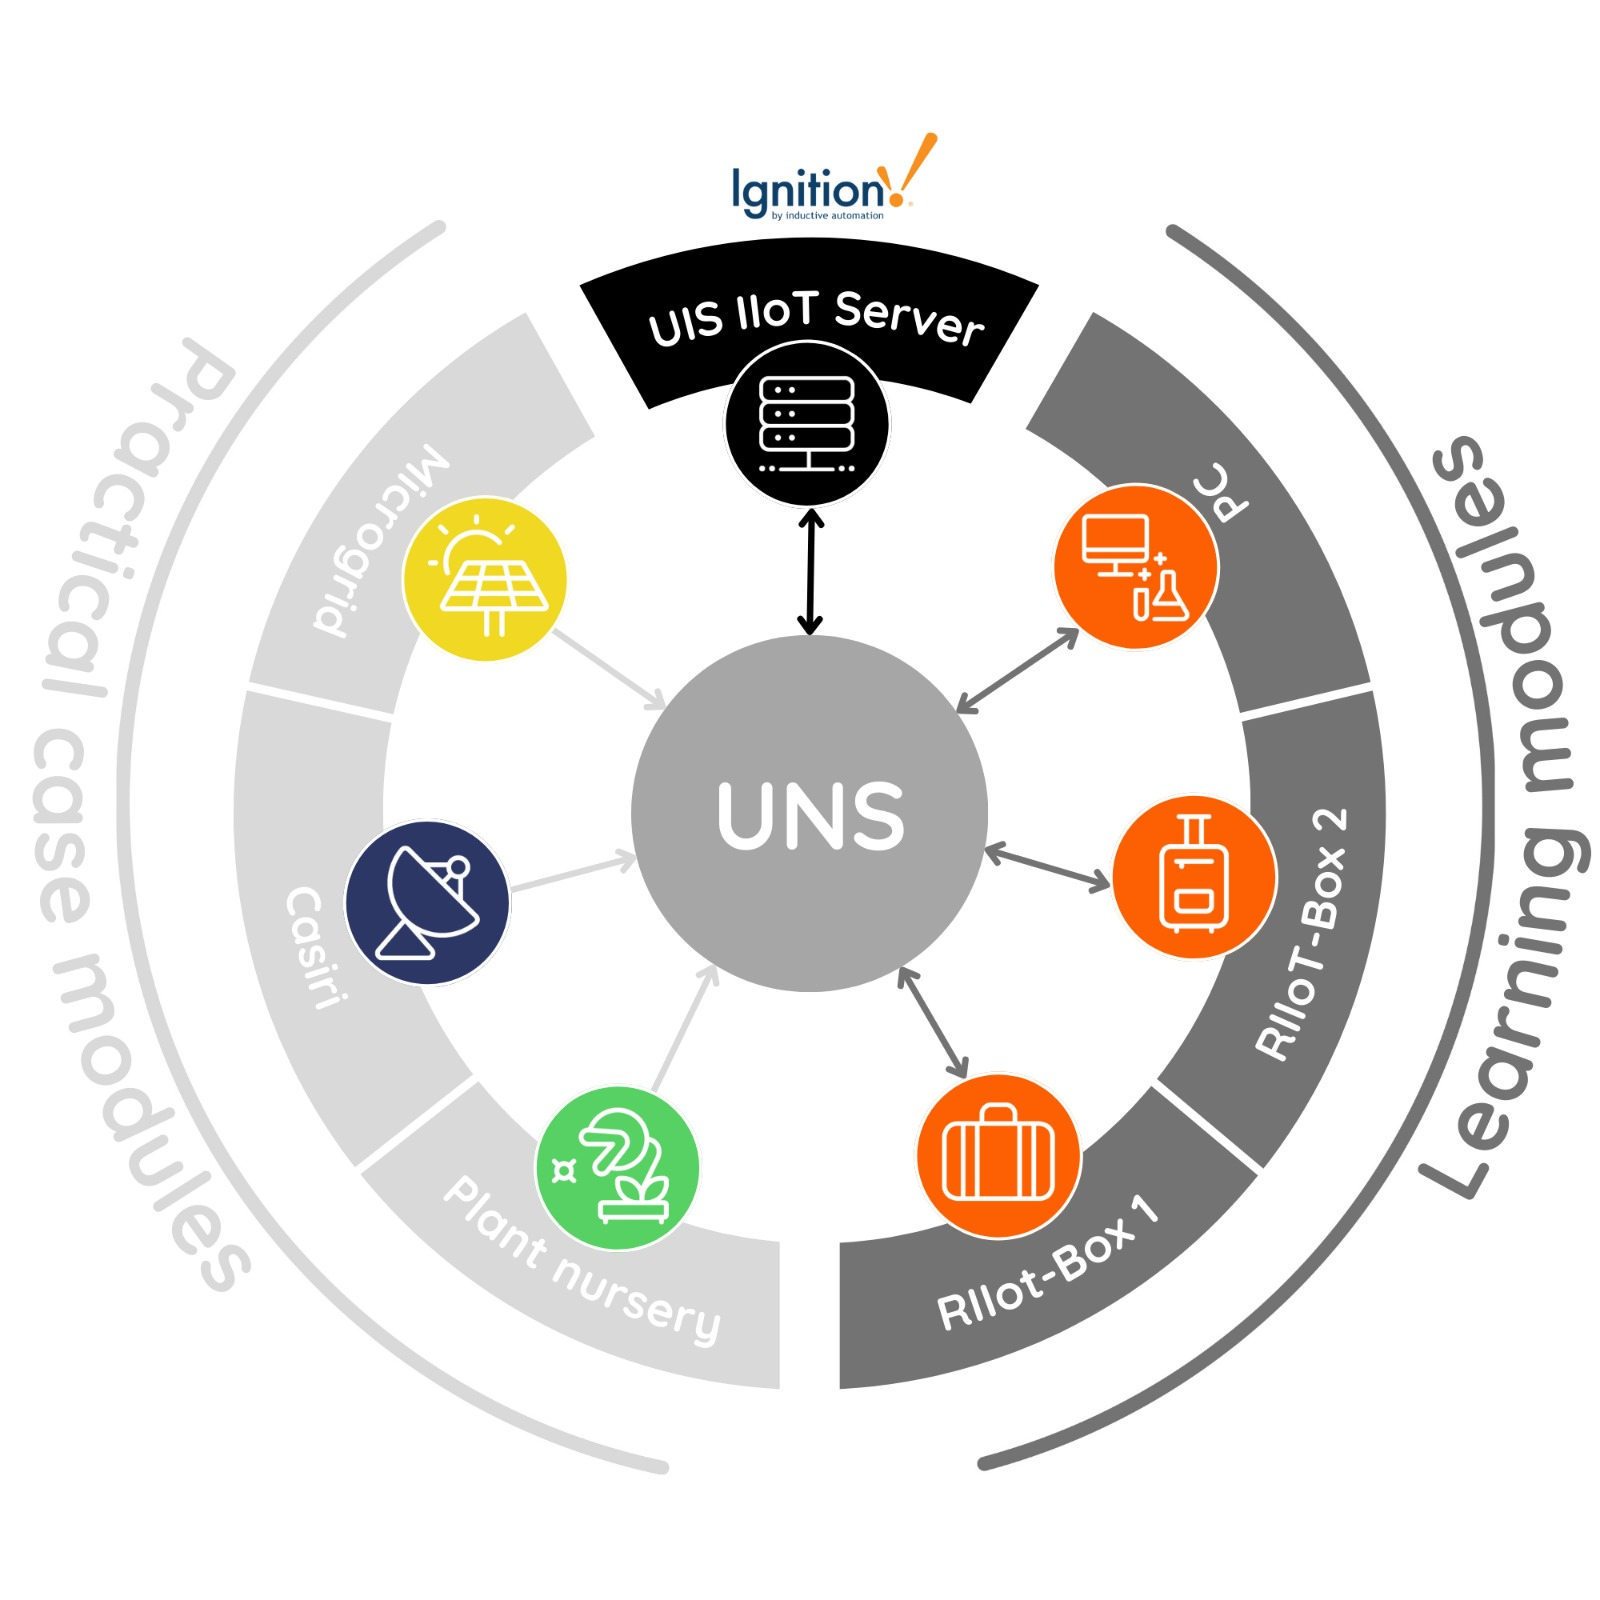
\includegraphics[width=10cm]{Figuras/IIoTPlatform_V2}}
\caption{Esquema de la Plataforma de Entrenamiento IIoT}
\label{fig:iiot_platform}
\end{figure}


Para centralizar la comunicación y visualización de datos en tiempo real de todos los dispositivos (casos de estudio) que actualmente se conectan de forma distribuida a través de internet, se propone implementar un UNS que sea el nodo central del sistema representado en la Figura \ref{fig:iiot_platform}. Allí se debe integrar un broker MQTT escalable a nivel de Enterprise mediante un servidor IIoT, con el objetivo de normalizar los datos, unificar protocolos y gestionar usuarios, permitiendo así una plataforma única para agregar, procesar y visualizar toda la información de los casos de estudio.\\

A partir de la conexión y configuración de los casos de estudio, es posible diseñar un UNS empleando las diversas técnicas de diseño previamente estudiadas y analizadas. Para cada caso, se define un \textit{namespace} estructurado, asegurando una organización eficiente de los datos y su interoperabilidad dentro del sistema.

Ambas metodologías se implementan utilizando el protocolo de comunicación MQTT Sparkplug B, lo que permite la integración de los casos de estudio al servidor principal de manera independiente. A continuación, se detalla el proceso de configuración en la plataforma.


\subsection{Implementación del Método Schultz}

Para la implementación de la técnica de Schultz, se establecen los niveles jerárquicos del UNS, organizando la arquitectura del sistema en función de los \textit{sites, areas, lines y cells} como se adquieren los datos. Esta estructura permite una gestión eficiente de la información para la integración de los dispositivos en la plataforma de entrenamiento IIoT.

El sistema está compuesto por dos \textit{sites} principales: Central y Guatiguará. En el \textit{site} Central, se encuentran dos \textit{areas} diferenciadas. La primera, Cenivam, comprende la \textit{line} Vivero y la \textit{cell} GroovRio, donde este último es el PLC encargado de la adquisición de datos a través del termo-higrómetro. La segunda \textit{area}, Radiogis, está conformada por la \textit{line} Casiri, las \textit{cell} Cámara, responsables de la captura de imágenes espectrales, y la \textit{cell} Estación Ambiental, que recopila información sobre variables ambientales.

Por otro lado, en el \textit{site} Guatiguará, se encuentra el \textit{area} LIE (Laboratorio de Integración Energética), la cual alberga la \textit{line} Microrred y la \textit{cell} GroovEpic, un PLC encargado de la adquisición de datos eléctricos de la Microrred.


\subsubsection{Arquitectura de Diseño}

Para implementar esta técnica en la aplicación de Ignition basada en MQTT Sparkplug B, se diseña la arquitectura mostrada en la Fig. \ref{fig:arqIIoT_Schultz}, en donde se escala desde el nivel de \textit{area}, al nivel de  \textit{site} y finalmente al nivel de \textit{Enterprise}.

\begin{figure}[H]
\centerline{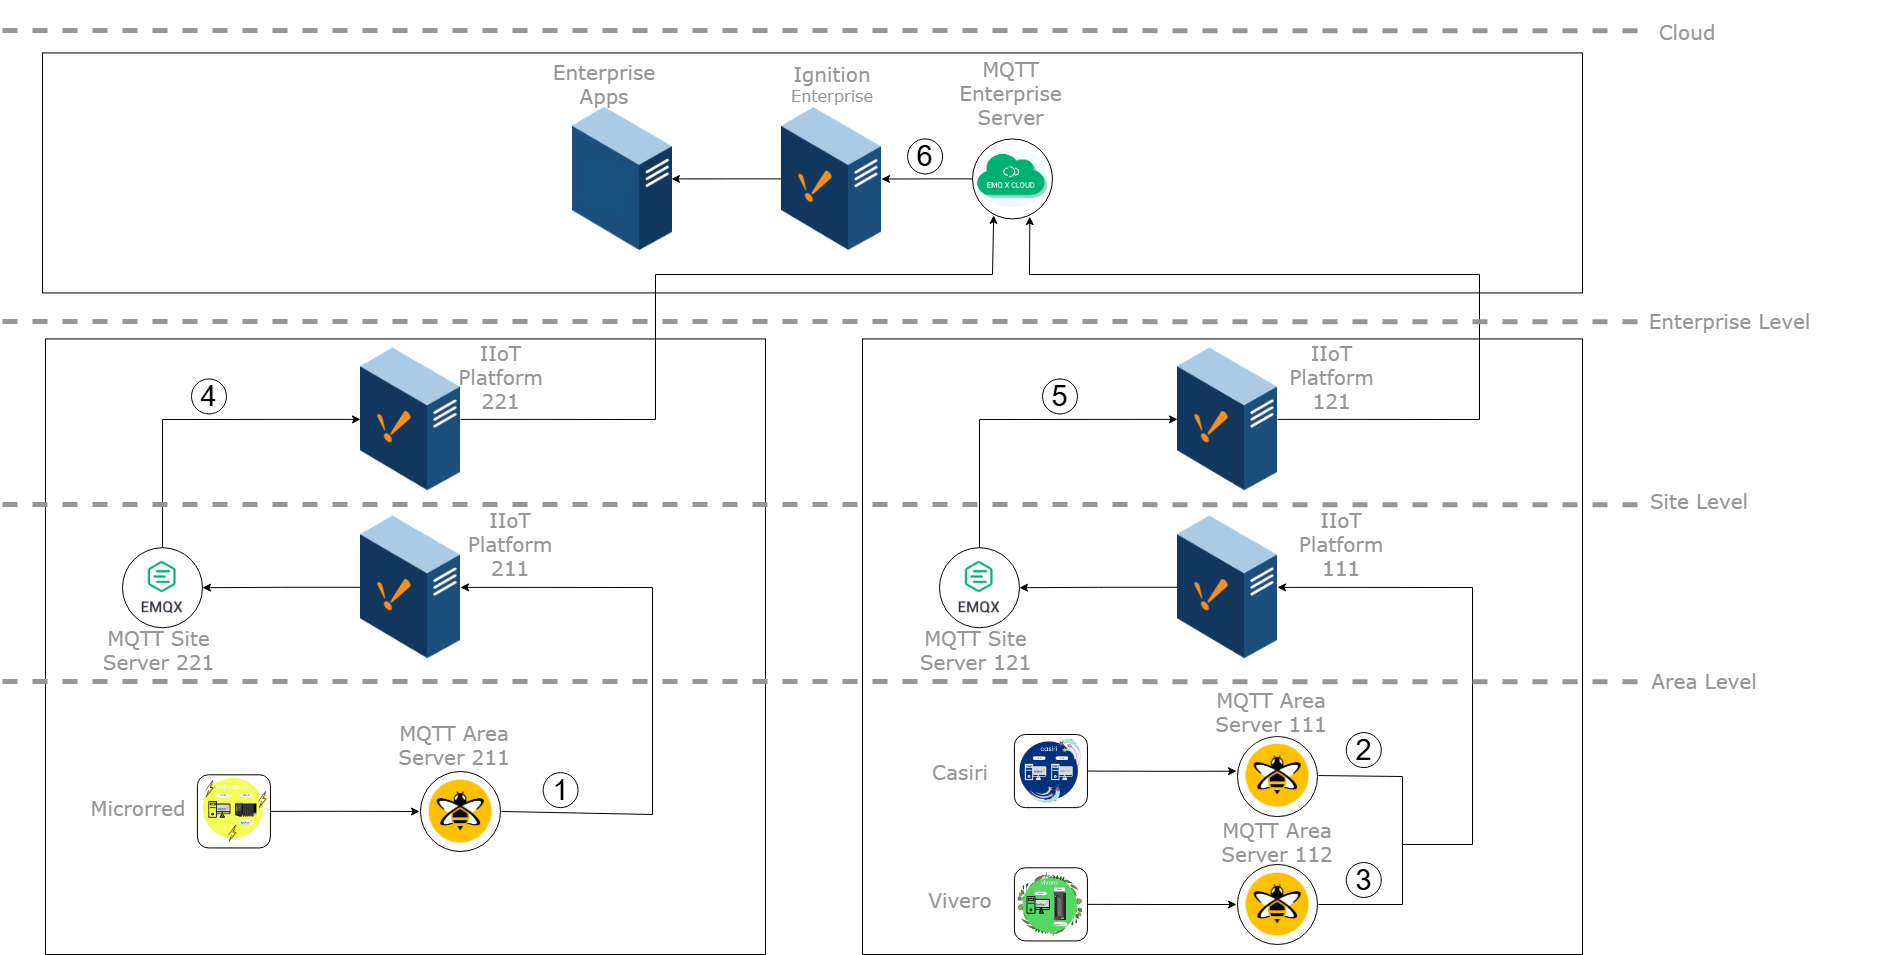
\includegraphics[width=19cm]{Figuras/ArqSchultz_IIoT_V3.png}}
\caption{Esquema de la Arquitectura UNS con el Método de Schultz en la Plataforma IIoT}
\label{fig:arqIIoT_Schultz}
\end{figure}


Los dispositivos IIoT de cada uno de los casos de estudio de la plataforma IIoT, se conectan a brokers de HiveMQ (MQTT Area Server 111, MQTT Area Server 112 y MQTT Site Server 211), que actúan como concentradores de datos para áreas específicas. Estos brokers recogen los datos y los envían a las Plataformas IIoT 111 y 211 para organizar los datos en un UNS de \textit{area} para cada caso, con la siguiente estructura: (\textcircled{1}, \textcircled{2} y \textcircled{3} en Fig. \ref{fig:arqIIoT_Schultz}) 

\begin{figure}[H]
\centering
\begin{minipage}{0.32\textwidth}
\centering
\scalebox{0.7}{
\begin{forest}
  for tree={
    font=\ttfamily,
    grow'=0,
    child anchor=west,
    parent anchor=south,
    anchor=west,
    calign=first,
    edge path={
      \noexpand\path [draw, \forestoption{edge}]
      (!u.south west) +(7.5pt,0) |- node[fill,inner sep=1.25pt] {} (.child anchor)\forestoption{edge label};
    },
    before typesetting nodes={
      if n=1
        {insert before={[,phantom]}}
        {}
    },
    fit=band,
    before computing xy={l=15pt},
  }
[\textbf{Area:} LIE
   [\textbf{Line:} Microrred
    [\textbf{Cell:} GroovEpic]
]
]
\end{forest}
}
\end{minipage}%
\begin{minipage}{0.32\textwidth}
\centering
\scalebox{0.7}{
\begin{forest}
  for tree={
    font=\ttfamily,
    grow'=0,
    child anchor=west,
    parent anchor=south,
    anchor=west,
    calign=first,
    edge path={
      \noexpand\path [draw, \forestoption{edge}]
      (!u.south west) +(7.5pt,0) |- node[fill,inner sep=1.25pt] {} (.child anchor)\forestoption{edge label};
    },
    before typesetting nodes={
      if n=1
        {insert before={[,phantom]}}
        {}
    },
    fit=band,
    before computing xy={l=15pt},
  }
[\textbf{Area:} Radiogis
   [\textbf{Line:} Casiri
    [\textbf{Cell:} Camara]
    [\textbf{Cell:} Estacion Ambiental]
]
]
\end{forest}
}
\end{minipage}%
\begin{minipage}{0.32\textwidth}
\centering
\scalebox{0.7}{
\begin{forest}
  for tree={
    font=\ttfamily,
    grow'=0,
    child anchor=west,
    parent anchor=south,
    anchor=west,
    calign=first,
    edge path={
      \noexpand\path [draw, \forestoption{edge}]
      (!u.south west) +(7.5pt,0) |- node[fill,inner sep=1.25pt] {} (.child anchor)\forestoption{edge label};
    },
    before typesetting nodes={
      if n=1
        {insert before={[,phantom]}}
        {}
    },
    fit=band,
    before computing xy={l=15pt},
  }
[\textbf{Area:} Cenivam
   [\textbf{Line:} Vivero
    [\textbf{Cell:} GroovRio]
]
]
\end{forest}
}
\end{minipage}
\end{figure}


%\begin{figure}[H] 
\centering
\scalebox{0.7}{
\begin{forest}
  for tree={
    font=\ttfamily,
    grow'=0,
    child anchor=west,
    parent anchor=south,
    anchor=west,
    calign=first,
    edge path={
      \noexpand\path [draw, \forestoption{edge}]
      (!u.south west) +(7.5pt,0) |- node[fill,inner sep=1.25pt] {} (.child anchor)\forestoption{edge label};
    },
    before typesetting nodes={
      if n=1
        {insert before={[,phantom]}}
        {}
    },
    fit=band,
    before computing xy={l=15pt},
  }
[\textbf{Area:} LIE
   [\textbf{Line:} Microrred
    [\textbf{Cell:} GroovEpic]
]
]
\end{forest}
}

\end{figure}

%\begin{figure}[H] 
\centering
\scalebox{0.7}{
\begin{forest}
  for tree={
    font=\ttfamily,
    grow'=0,
    child anchor=west,
    parent anchor=south,
    anchor=west,
    calign=first,
    edge path={
      \noexpand\path [draw, \forestoption{edge}]
      (!u.south west) +(7.5pt,0) |- node[fill,inner sep=1.25pt] {} (.child anchor)\forestoption{edge label};
    },
    before typesetting nodes={
      if n=1
        {insert before={[,phantom]}}
        {}
    },
    fit=band,
    before computing xy={l=15pt},
  }
[\textbf{Area:} Radiogis
   [\textbf{Line:} Casiri
    [\textbf{Cell:} Camara]
    [\textbf{Cell:} Estacion Ambiental]
]
]
\end{forest}
}

\end{figure}

%\begin{figure}[H] 
\centering
\scalebox{0.7}{
\begin{forest}
  for tree={
    font=\ttfamily,
    grow'=0,
    child anchor=west,
    parent anchor=south,
    anchor=west,
    calign=first,
    edge path={
      \noexpand\path [draw, \forestoption{edge}]
      (!u.south west) +(7.5pt,0) |- node[fill,inner sep=1.25pt] {} (.child anchor)\forestoption{edge label};
    },
    before typesetting nodes={
      if n=1
        {insert before={[,phantom]}}
        {}
    },
    fit=band,
    before computing xy={l=15pt},
  }
[\textbf{Area:} Cenivam
   [\textbf{Line:} Vivero
    [\textbf{Cell:} GroovRio]
]
]
\end{forest}
}

\end{figure}


Secuencialmente, los UNS de \textit{area} son enviados a un broker local (MQTT Site Server 121 y 221) para recolectar la información por \textit{site} y enviarlas a las Plataformas IIoT 121 y 221. Estas procesan los datos contextualizados y organizan los datos en un UNS de \textit{site} con la siguiente estructura:(\textcircled{4} y  \textcircled{5} en Fig. \ref{fig:arqIIoT_Schultz}))\\

\begin{figure}[H]
\centering
\begin{minipage}{0.32\textwidth}
\centering
\scalebox{0.6}{
\begin{forest}
  for tree={
    font=\ttfamily,
    grow'=0,
    child anchor=west,
    parent anchor=south,
    anchor=west,
    calign=first,
    edge path={
      \noexpand\path [draw, \forestoption{edge}]
      (!u.south west) +(7.5pt,0) |- node[fill,inner sep=1.25pt] {} (.child anchor)\forestoption{edge label};
    },
    before typesetting nodes={
      if n=1
        {insert before={[,phantom]}}
        {}
    },
    fit=band,
    before computing xy={l=15pt},
  }
  [\textbf{Site:} Guatiguara  
    [\textbf{Area:} LIE
       [\textbf{Line:} Microrred
        [\textbf{Cell:} GroovEpic]
       ]
    ]
  ]
\end{forest}
}
\end{minipage}%
\begin{minipage}{0.32\textwidth}
\centering
\scalebox{0.6}{
\begin{forest}
  for tree={
    font=\ttfamily,
    grow'=0,
    child anchor=west,
    parent anchor=south,
    anchor=west,
    calign=first,
    edge path={
      \noexpand\path [draw, \forestoption{edge}]
      (!u.south west) +(7.5pt,0) |- node[fill,inner sep=1.25pt] {} (.child anchor)\forestoption{edge label};
    },
    before typesetting nodes={
      if n=1
        {insert before={[,phantom]}}
        {}
    },
    fit=band,
    before computing xy={l=15pt},
  }
[\textbf{Site:} Central
    [\textbf{Area:} Radiogis
       [\textbf{Line:} Casiri
        [\textbf{Cell:} Camara]
        [\textbf{Cell:} Estacion Ambiental]
       ]
    ]
    [\textbf{Area:} Cenivam
       [\textbf{Line:} Vivero
        [\textbf{Cell:} GroovRio]
       ]
    ]
]
\end{forest}
}
\end{minipage}
\end{figure}



Finalmente, con la estructura definida para cada uno de los \textit{site}, se consolidan todos los namespaces distribuidos en un broker en la nube (MQTT Enterprise Server). Este recibe todas las áreas de la infraestructura y organiza el UNS a nivel de \textit{Enterprise} en el Ignition Enterprise, con el siguiente modelo jerárquico.(\textcircled{6} en Fig. \ref{fig:arqIIoT_Schultz}) 

\begin{figure}[H] 
\centering
\scalebox{0.7}{
\begin{forest}
  for tree={
    font=\ttfamily,
    grow'=0,
    child anchor=west,
    parent anchor=south,
    anchor=west,
    calign=first,
    edge path={
      \noexpand\path [draw, \forestoption{edge}]
      (!u.south west) +(7.5pt,0) |- node[fill,inner sep=1.25pt] {} (.child anchor)\forestoption{edge label};
    },
    before typesetting nodes={
      if n=1
        {insert before={[,phantom]}}
        {}
    },
    fit=band,
    before computing xy={l=15pt},
  }
[\textbf{Enterprise:} UIS
  [\textbf{Site:} Central
    [\textbf{Area:} Cenivam
        [\textbf{Line:} Vivero
            [\textbf{Cell:} GroovRio]
        ]
    ]
    [\textbf{Area:} Radiogis 
        [\textbf{Line:} Casiri
            [\textbf{Cell:} Camara]
            [\textbf{Cell:} Estacion Ambiental]
        ]
    ]
]
   [\textbf{Site:} Guatiguara
    [\textbf{Area:} LIE
        [\textbf{Line:} Microrred
            [\textbf{Cell:} GroovEpic]
        ]
    ]
]
]
\end{forest}
}

\end{figure}


La nube opera como la capa de integración global, permitiendo analítica avanzada y gestión remota de cada uno de los niveles de la jerarquía, además permite la conexión de diferentes aplicaciones al nivel de \textit{Enterprise} para monitorear y controlar los datos. Esta estructura multi-capa mantiene la autonomía local, evita los diferentes silos de datos y permite la re-conexión automática de los datos ante una falla en el sistema en cualquier nivel del UNS.

\subsubsection{Implementación en Ignition}

Una vez diseñada e implementada la arquitectura del UNS utilizando el método de Schultz, es posible establecer conexión con el servidor Enterprise MQTT a través de la aplicación Ignition. Esta conexión permite visualizar de forma estructurada y en tiempo real toda la jerarquía del UNS previamente definida, facilitando el acceso a los datos organizados por \textit{sites}, \textit{areas}, \textit{lines} y \textit{cells}. La plataforma Ignition actúa como cliente MQTT compatible con Sparkplug B, lo que permite la exploración y supervisión directa del modelo UNS. A continuación, se presenta una visualización dentro del entorno de Ignition.

\begin{figure}[h]
\centerline{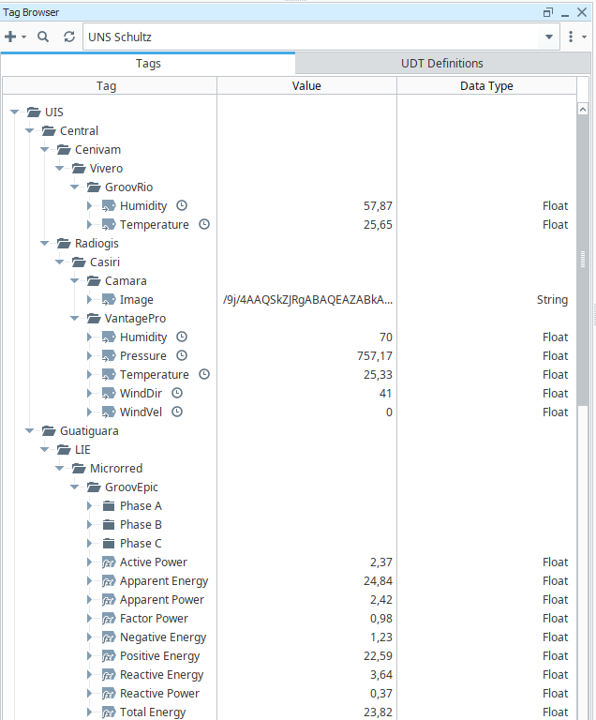
\includegraphics[width=8cm]{Figuras/UNS_Schultz_Ignition}}
\caption{UNS Schultz en Ignition}
\label{fig:unsSchultzig}
\end{figure}

A través de esta estructura jerárquica es posible acceder a los datos de toda la infraestructura, desde el nivel \textit{Enterprise} hasta el nivel de \textit{cell}, reflejando con precisión los distintos niveles definidos en el UNS. Cada uno de estos niveles representa una instancia clara dentro de la jerarquía del sistema, lo que garantiza una organización coherente y uniforme de los dispositivos y sensores conectados en las diferentes áreas.

Esta estandarización en la representación y ubicación de los dispositivos permite lograr una alta escalabilidad e interoperabilidad sin necesidad de modificar la arquitectura base. De esta manera, cualquier nuevo caso de estudio o integración de un dispositivo adicional puede ser incorporado directamente en el área correspondiente, y automáticamente será reflejado en el UNS general, manteniendo la integridad y consistencia del sistema.

\subsection{Implementación del Método Parris}

Para la aplicación de la técnica de Parris en la plataforma IIoT, se define la jerarquía del UNS replicando la estructura utilizada previamente, basada en los mismos \textit{sites}, \textit{areas}, \textit{lines} y \textit{cells} de adquisición de datos de la plataforma. La arquitectura contempla nuevamente dos \textit{sites} principales: Central, que incluye las \textit{areas} Cenivam, con la \textit{line} Vivero y la \textit{cell} GroovRio, además del Radiogis, con la \textit{line} Casiri y las \textit{cells} Cámara y Estación Ambiental; por otro lado, se tiene el \textit{site} Guatiguará, que incorpora el \textit{area} LIE, compuesta por la \textit{line} Microrred y la \textit{cell} GroovEpic.

\subsubsection{Arquitectura de Diseño}

La arquitectura basada en el método de Parris presenta un enfoque simplificado y estandarizado para implementar un UNS, utilizando un broker MQTT centralizado como columna vertebral de la comunicación. A diferencia del modelo jerárquico de Schultz, aquí todos los dispositivos (Sensor 1, Sensor 2, Sensor 3) de los 3 casos de estudios y las aplicaciones (como Ignition Enterprise) se conectan directamente al mismo MQTT Broker en la nube, eliminando capas intermedias de servidores locales. En la Fig. \ref{fig:arqIIoT_Parris} se representa como cada dispositivo publica datos en rutas estandarizadas (UNS Path) para cada uno de los casos, que definen un namespace unificado y accesible para toda la organización. Algunos ejemplos de UNS Path utilizando el delimitador \textit{"\_"} son los siguientes:


\begin{center}
    UNS Path 1: \textit{UIS\_Central/Radiogis\_Casiri\_Estacion Ambiental/<device\_id>}\\
    UNS Path 2: \textit{UIS\_Central/Cenivam\_Vivero\_GroovRio/<device\_id>}\\
    UNS Path 3: \textit{UIS\_Guatiguara/LIE\_Microrred\_GroovEpic/<device\_id>}
\end{center}



\begin{figure}[H]
\centerline{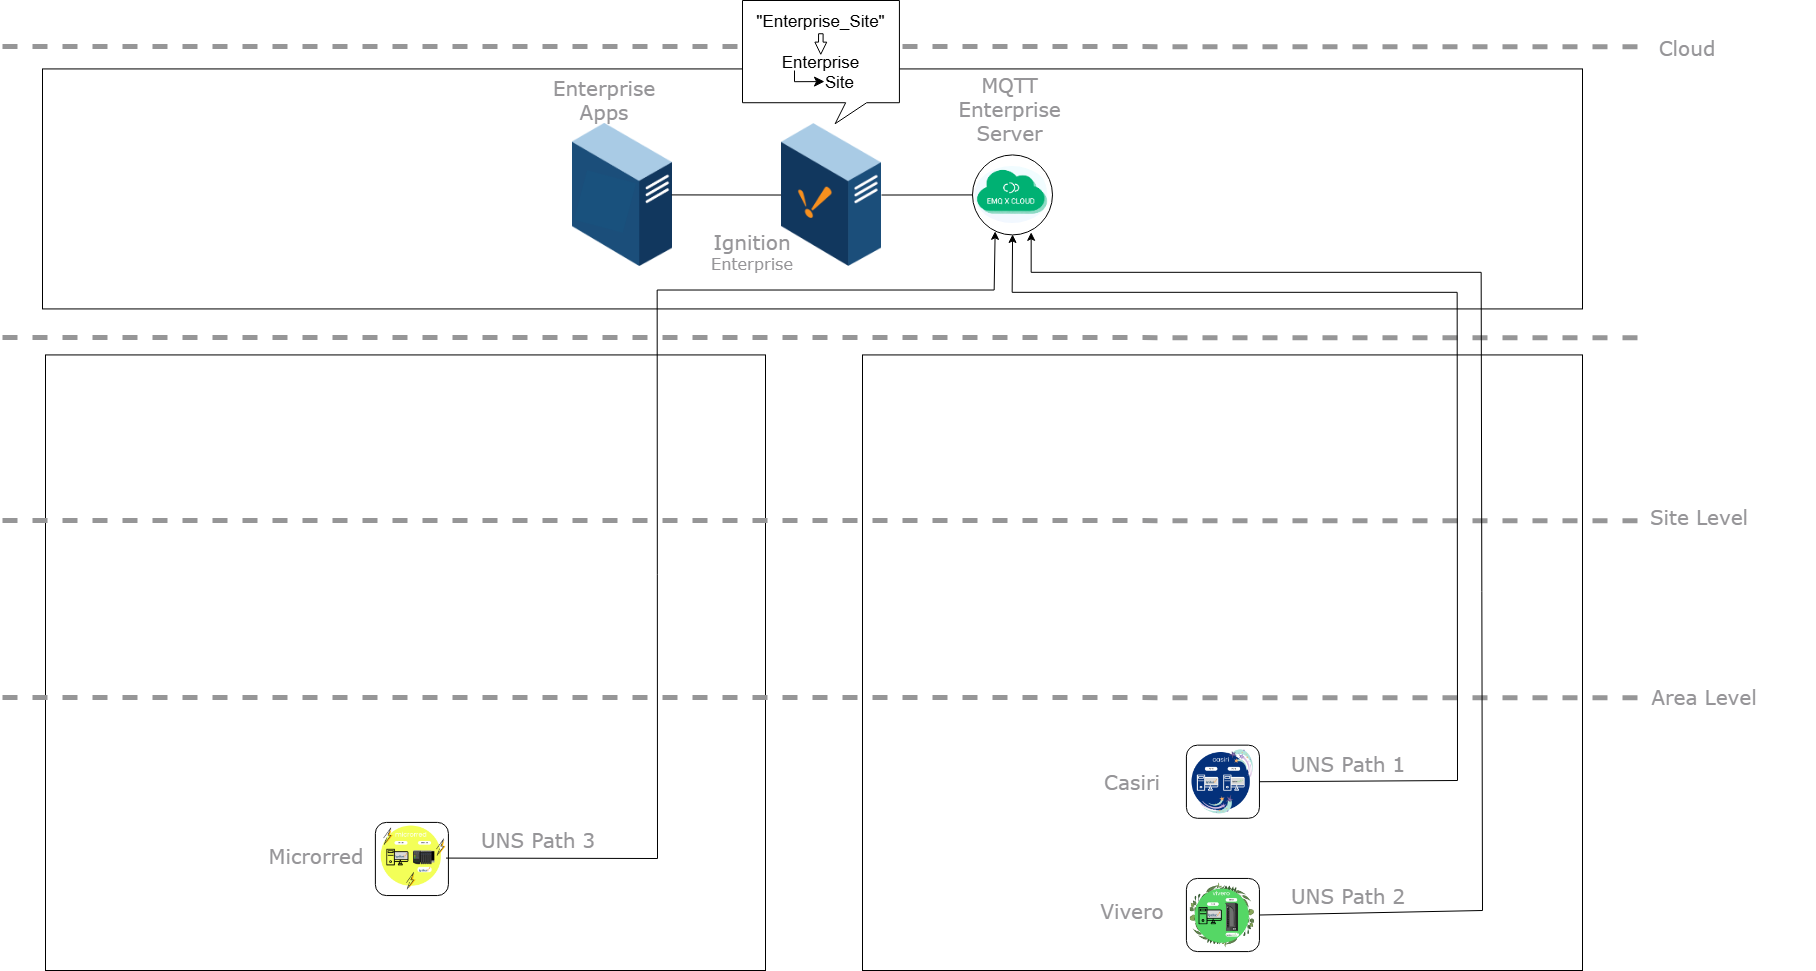
\includegraphics[width=19cm]{Figuras/ArqParris_IIoT_V3.png}}
\caption{Esquema de la Arquitectura UNS con el Metodo de Parris en la Plataforma IIoT}
\label{fig:arqIIoT_Parris}
\end{figure}


Las aplicaciones acceden directamente al broker central para visualizar, analizar y controlar los datos en tiempo real. De manera similar al método de Schultz, la jerarquía del UNS diseñada desde la plataforma Ignition Enterprise se representa con la siguiente estructura.

\begin{figure}[H] 
\centering
\scalebox{0.7}{
\begin{forest}
  for tree={
    font=\ttfamily,
    grow'=0,
    child anchor=west,
    parent anchor=south,
    anchor=west,
    calign=first,
    edge path={
      \noexpand\path [draw, \forestoption{edge}]
      (!u.south west) +(7.5pt,0) |- node[fill,inner sep=1.25pt] {} (.child anchor)\forestoption{edge label};
    },
    before typesetting nodes={
      if n=1
        {insert before={[,phantom]}}
        {}
    },
    fit=band,
    before computing xy={l=15pt},
  }
[\textbf{Enterprise:} UIS
  [\textbf{Site:} Central
    [\textbf{Area:} Cenivam
        [\textbf{Line:} Vivero
            [\textbf{Cell:} GroovRio]
        ]
    ]
    [\textbf{Area:} Radiogis 
        [\textbf{Line:} Casiri
            [\textbf{Cell:} Camara]
            [\textbf{Cell:} Estacion Ambiental]
        ]
    ]
]
   [\textbf{Site:} Guatiguara
    [\textbf{Area:} LIE
        [\textbf{Line:} Microrred
            [\textbf{Cell:} GroovEpic]
        ]
    ]
]
]
\end{forest}
}

\end{figure}



El método de Parris destaca por su simplicidad y flexibilidad, ideal para entornos donde la agilidad y la conectividad directa son prioritarias. Al eliminar servidores intermedios, se reduce el mantenimiento y se acelera la implementación, aunque requiere un broker MQTT robusto y una red confiable para manejar todo el tráfico de datos de manera eficiente.



\subsubsection{Implementación  en Ignition}

Una vez implementada la arquitectura del UNS, se establece la conexión con el broker MQTT centralizado, el cual contiene la estructura completa del sistema. A través de la aplicación Ignition, es posible visualizar cada uno de los ``Paths'' correspondientes a los casos de estudio, estructurados según el delimitador definido. Esta visualización se realiza conforme a la especificación MQTT Sparkplug B, adoptando la siguiente organización jerárquica:

\begin{center}      
    \textit{<group\_id>: Enterprise\_Site}\\ 
    \textit{<edgenode\_id>: Area\_Line\_Cell}\\ 
\end{center}

En la Fig \ref{fig:unsParrisig_engine} se puede observar como se reciben los topics en Ignition según la especificación del protocolo y la definición de cada uno de los nodos.


\begin{figure}[H]
\centerline{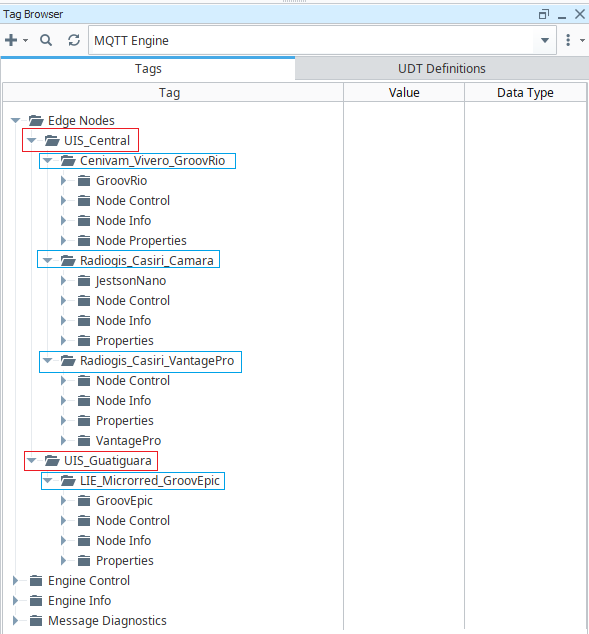
\includegraphics[width=8cm]{Figuras/UNS_Engine_Parris_Ignition_V2}}
\caption{Método de Parris en el Módulo MQTT Engine en Ignition}
\label{fig:unsParrisig_engine}
\end{figure}

La aplicación permite recibir y procesar los ``topics''
suscritos, y como se muestra en la Fig. \ref{fig:unsParrisig}, Ignition interpreta los delimitadores ``\_'' para dividirlos en sub-topics, construyendo así la jerarquía del UNS definida previamente.


\begin{figure}[H]
\centerline{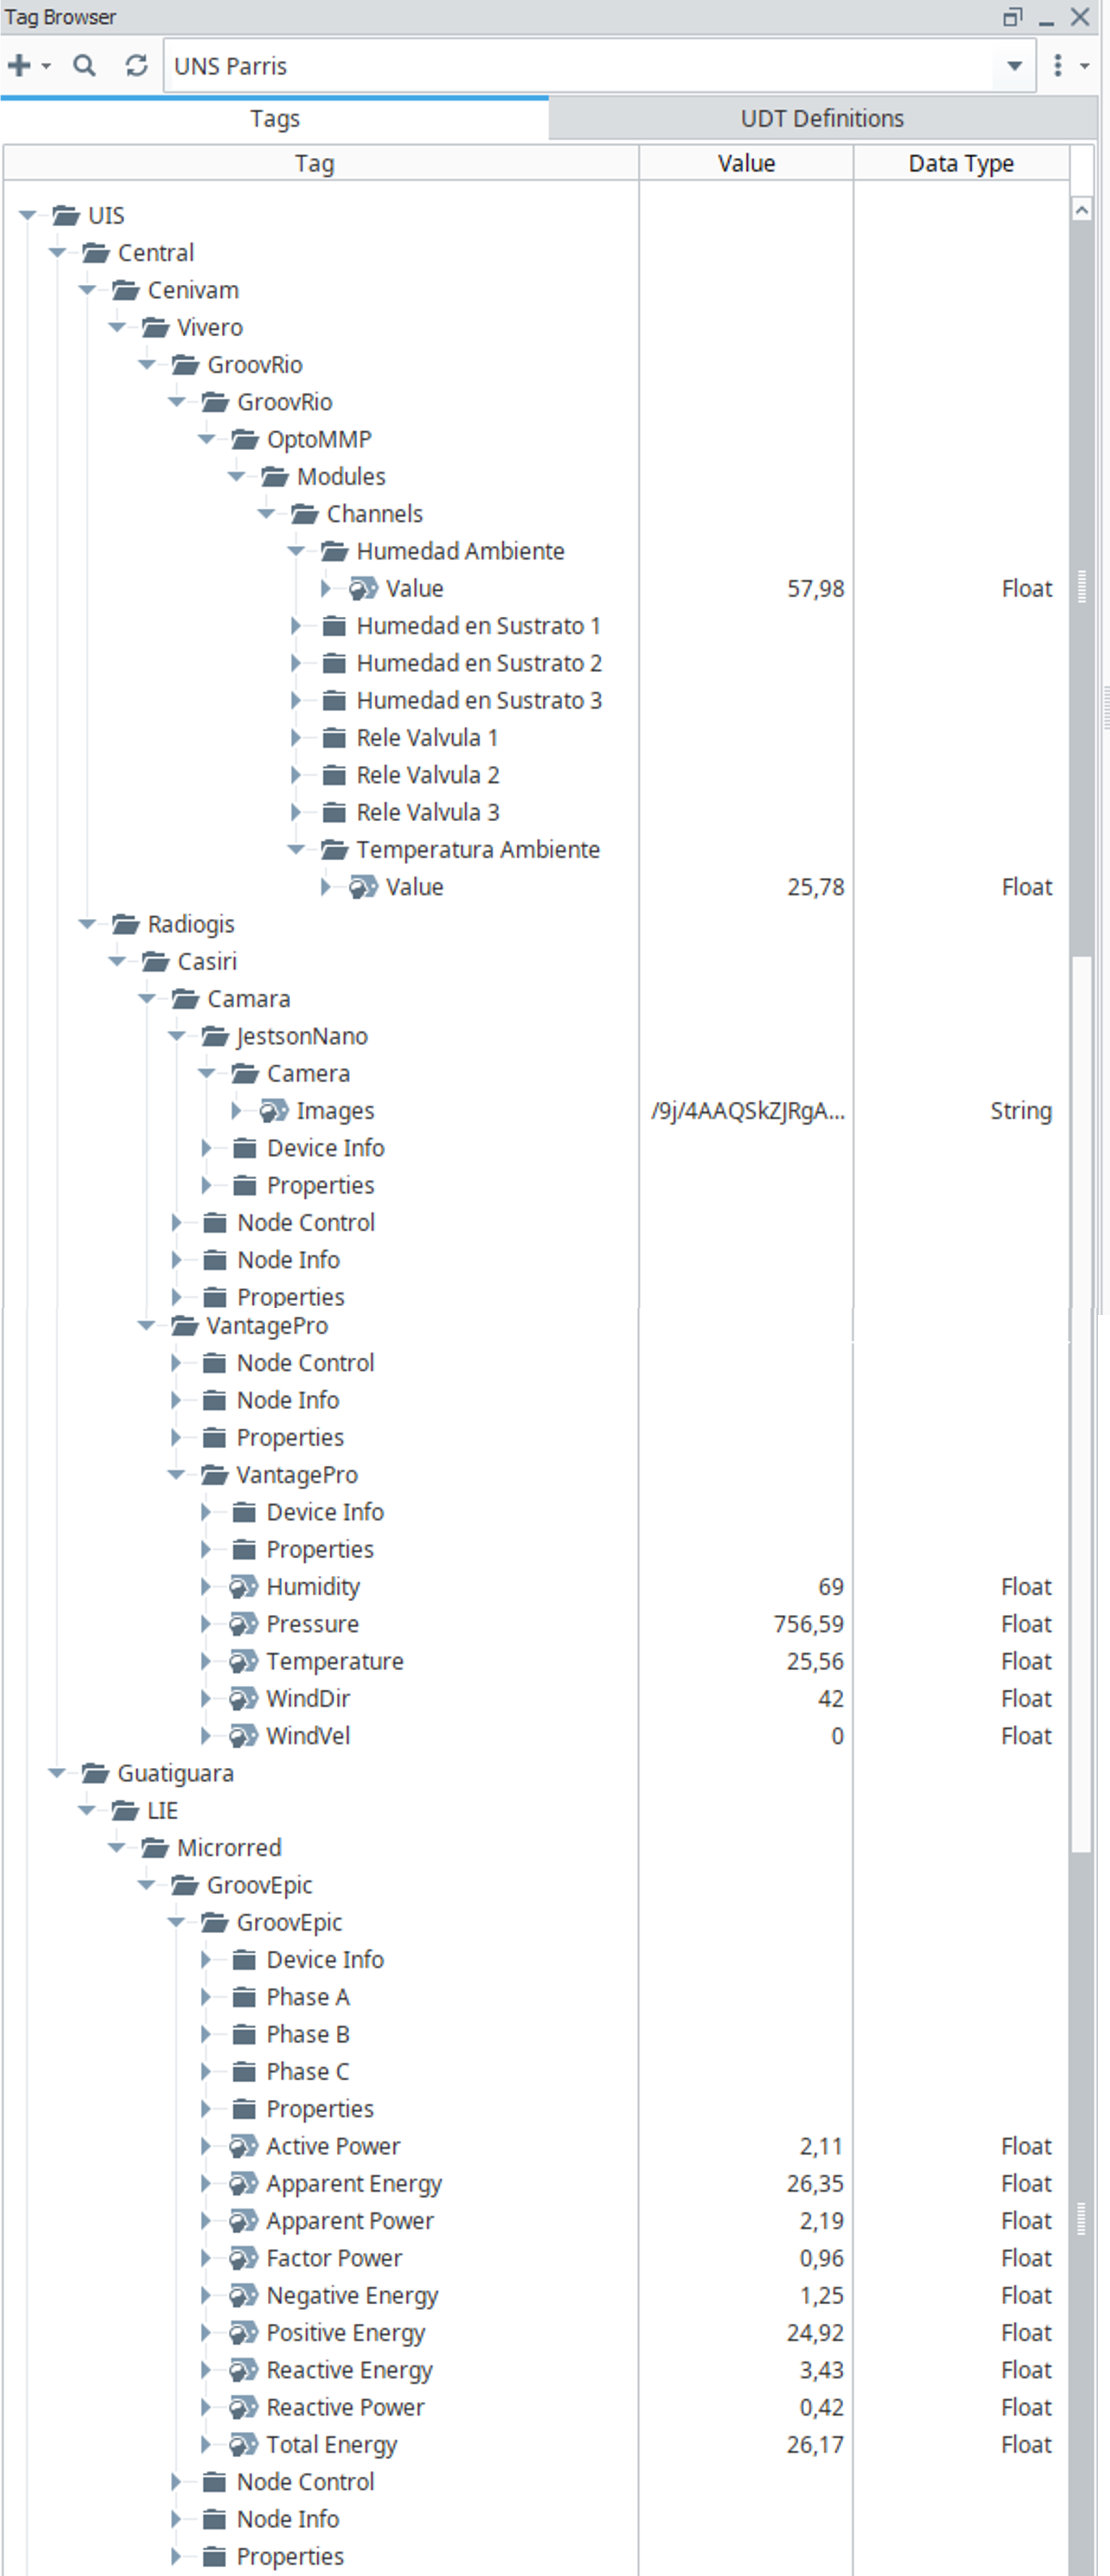
\includegraphics[width=7.9cm]{Figuras/UNS_Parris_Ignition}}
\caption{Método de Parris Estructurado en Ignition}
\label{fig:unsParrisig}
\end{figure}



\subsection{Aplicación Ignition Plataforma IIoT}

La plataforma Ignition actúa como interfaz de visualización dentro de la arquitectura IIoT basada en Unified Namespace, proporcionando al usuario final acceso estructurado a los datos del sistema. En esta etapa, se detalla el diseño del \textit{Front-End} de la aplicación, incluyendo la disposición de vistas, widgets e indicadores interactivos que permiten la supervisión, análisis y control operativo en tiempo real de forma eficiente e intuitiva.

La vista principal de la aplicación corresponde al Home, como se muestra en la Figura \ref{fig:homeUNS}. Esta pantalla centraliza el acceso a los distintos módulos de monitoreo, permitiendo navegar de forma intuitiva entre los distintos sites y componentes del sistema.

\begin{figure}[H]
\centerline{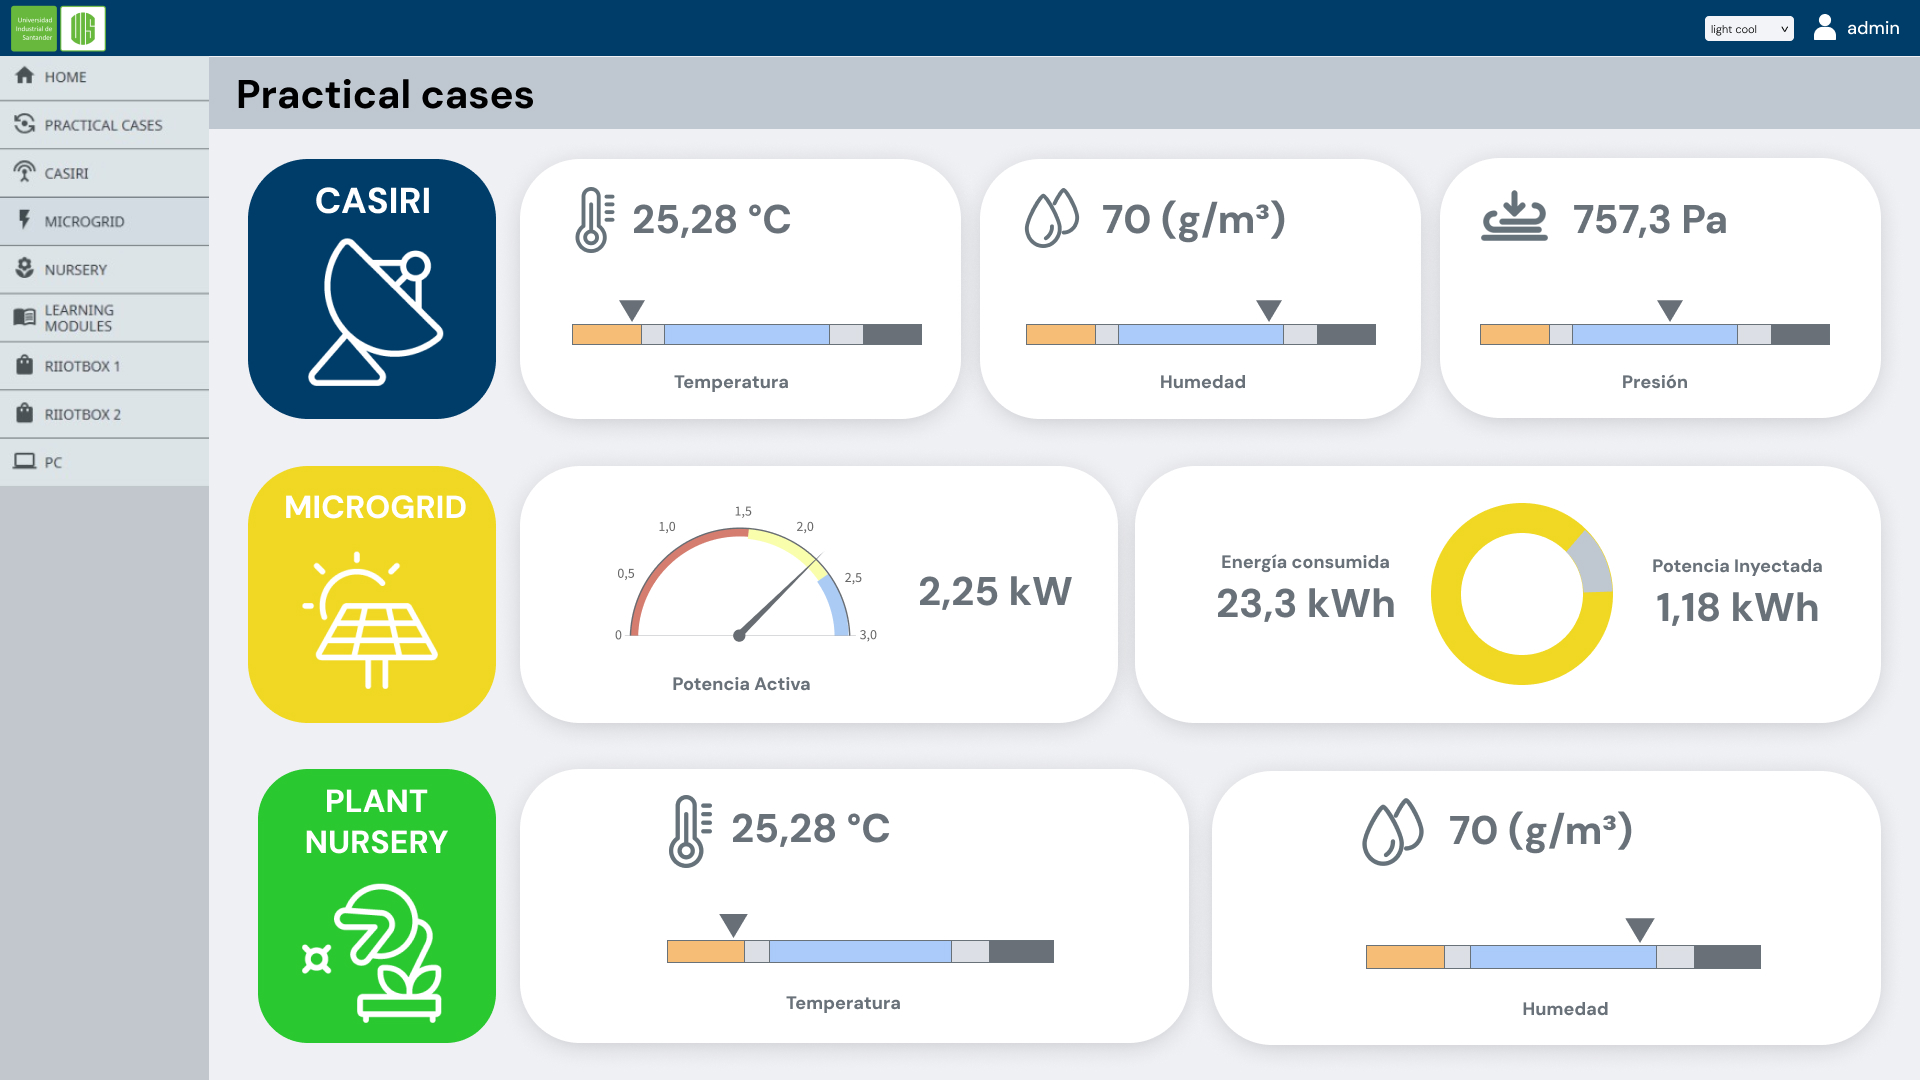
\includegraphics[width=15cm]{Figuras/HomeUNS}}
\caption{Vista del Home en la aplicación de Ignition}
\label{fig:homeUNS}
\end{figure}


La Figura \ref{fig:casiriView} muestra la visualización correspondiente a Casiri, dentro del área Radiogis del site Central. En esta vista, se monitorean variables ambientales capturadas por la Estación Ambiental y se obtienen las imágenes capturadas por la Cámara espectral, presentando los datos en tiempo real mediante gráficos e indicadores analógicos y datos históricos.


\begin{figure}[H]
\centerline{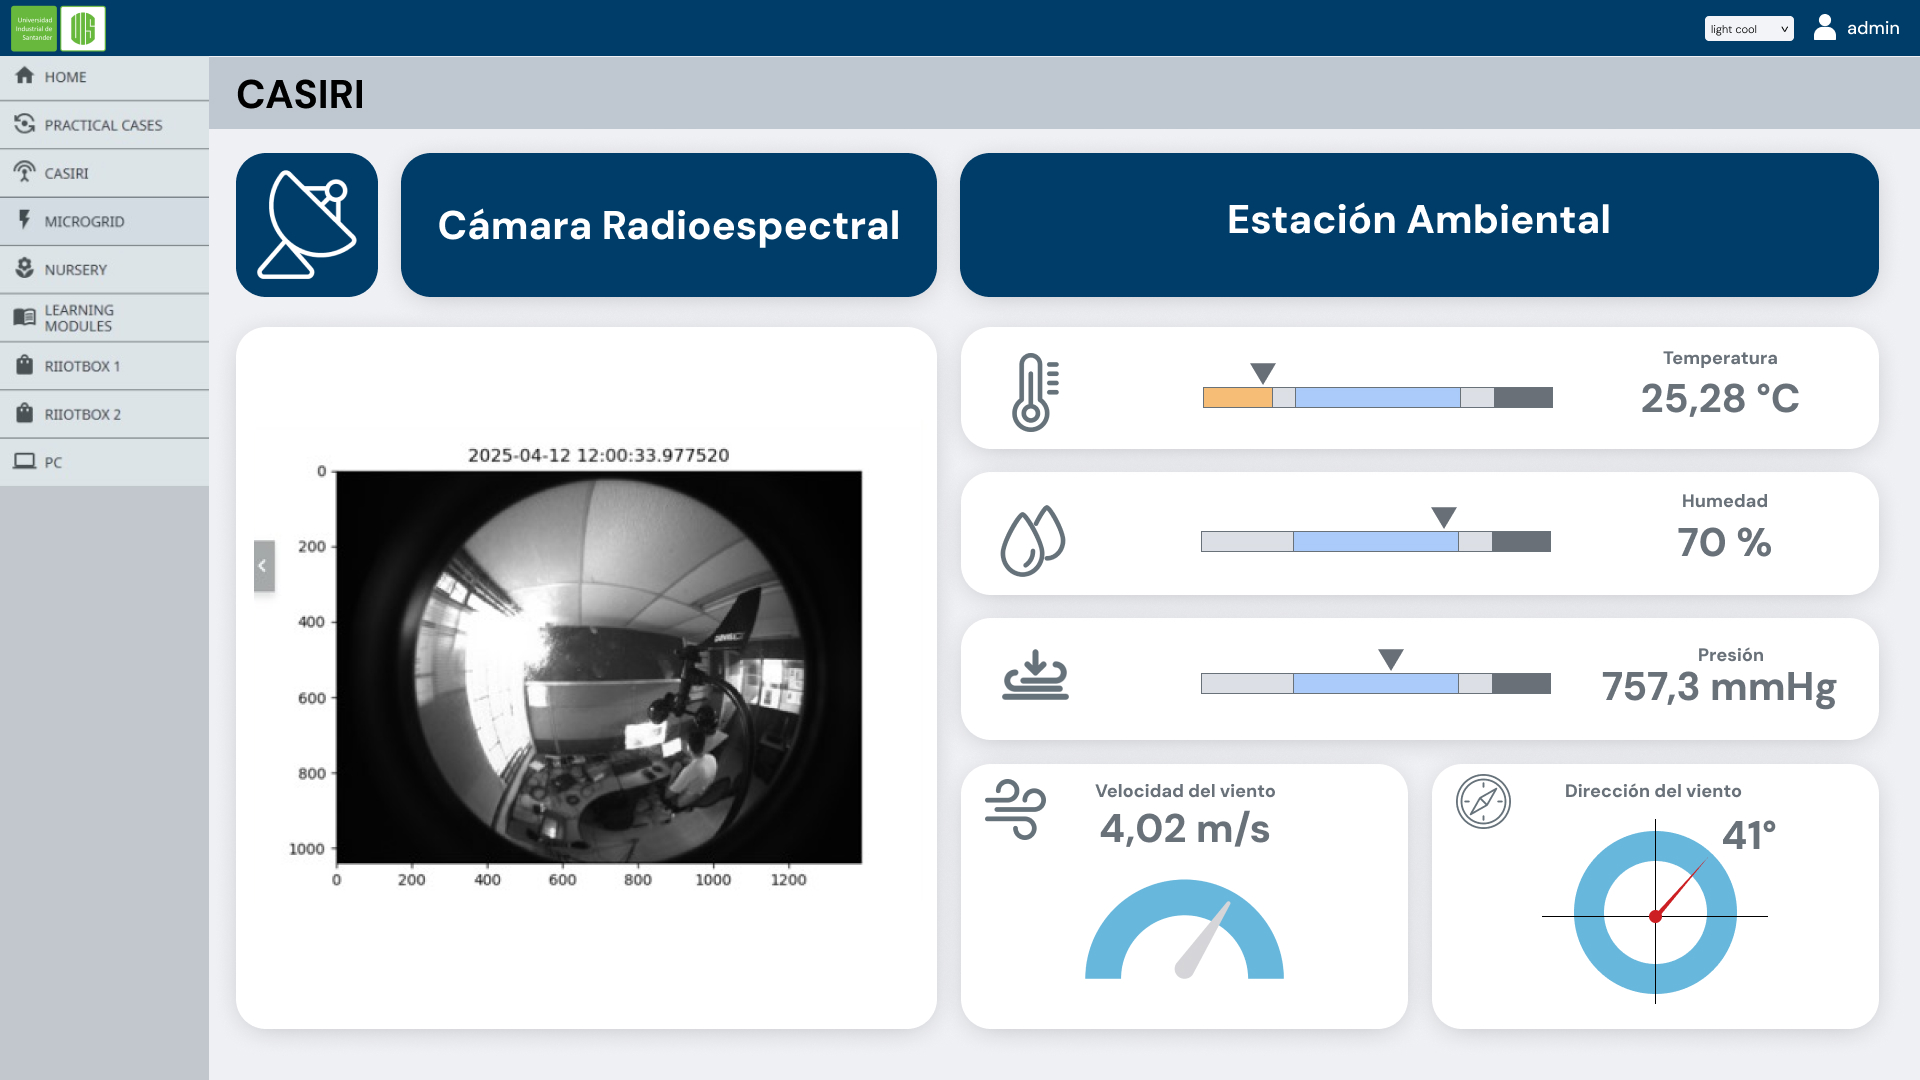
\includegraphics[width=14.1cm]{Figuras/ViewCasiri}}
\caption{Vista de Casiri en la aplicación de Ignition}
\label{fig:casiriView}
\end{figure}


En la Figura \ref{fig:microrredView}, se ilustra la vista de la Microrred, ubicada en el área LIE del site Guatiguará. Esta vista permite observar el comportamiento eléctrico de cada una de las fases de la Microrred que permite leer el PLC GroovEpic, representando variables claves del sistema.

\begin{figure}[H]
\centerline{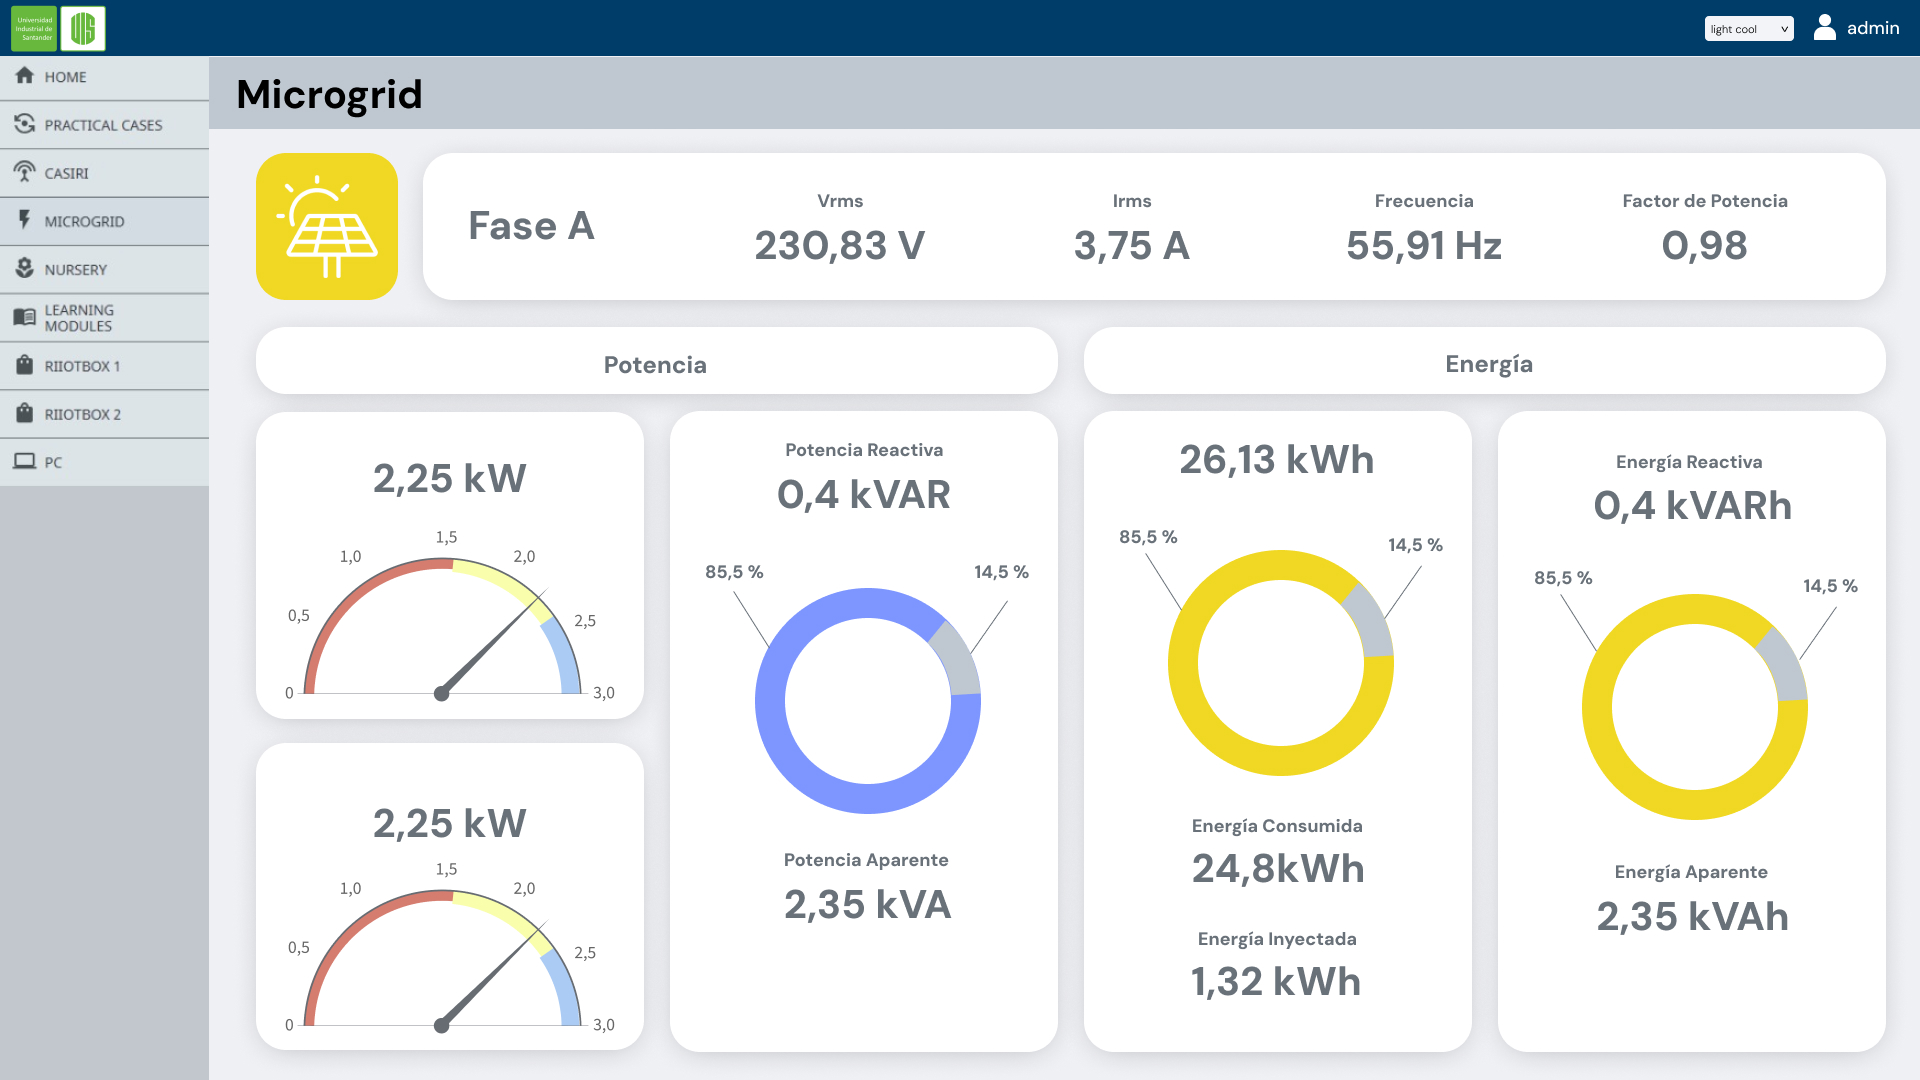
\includegraphics[width=14.1cm]{Figuras/ViewMicrorred}}
\caption{Vista de la Microrred en la aplicación de Ignition}
\label{fig:microrredView}
\end{figure}



Finalmente, la Figura \ref{fig:viveroView} corresponde a la vista del Vivero, parte del área Cenivam del site Central. En esta interfaz se visualizan parámetros ambientales recolectados por el termo-higrómetro a través del PLC GroovRio, permitiendo una supervisión detallada de las condiciones del entorno y un historial de cada una de ellas.

\begin{figure}[H]
\centerline{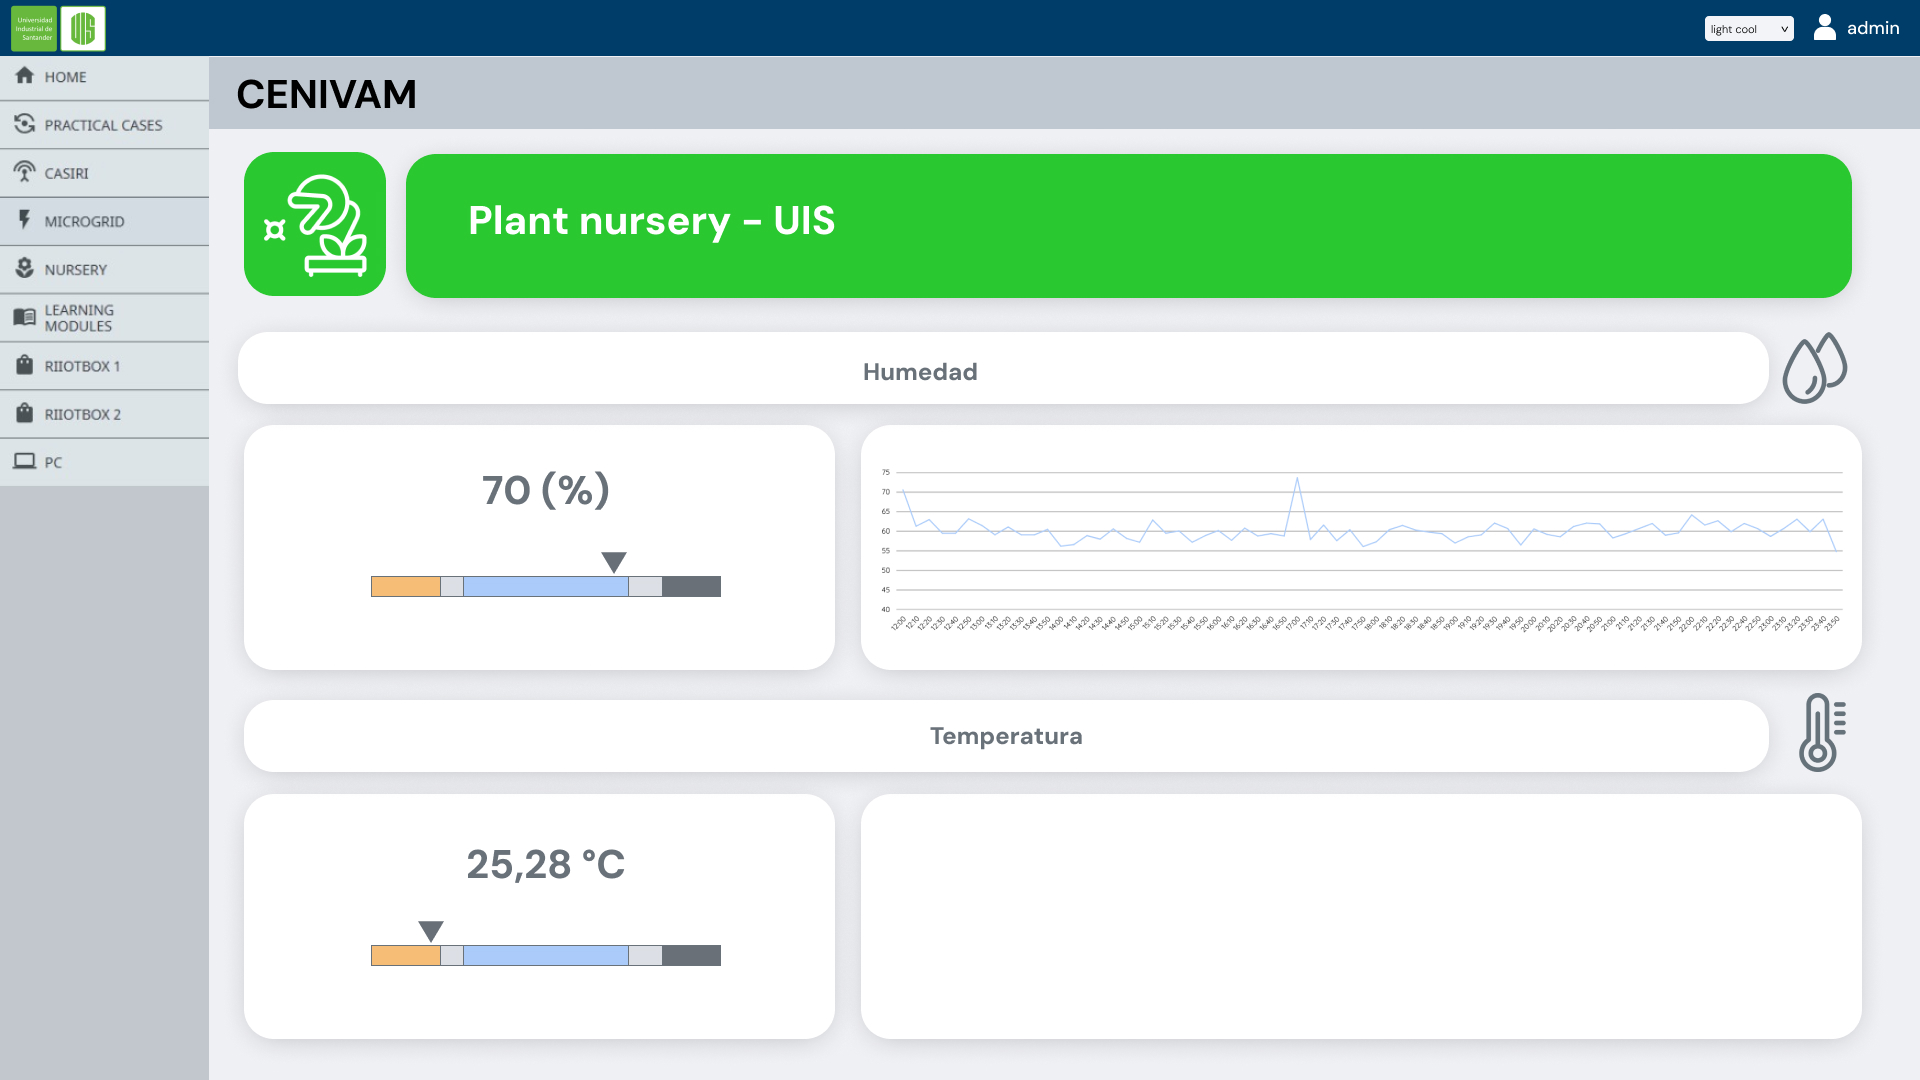
\includegraphics[width=15cm]{Figuras/ViewCenivam}}
\caption{Vista del Vivero en la aplicación de Ignition}
\label{fig:viveroView}
\end{figure}

Estas interfaces gráficas están diseñadas para ofrecer una interacción eficiente y en tiempo real entre el usuario y el sistema, permitiendo la supervisión y análisis de los datos mediante una visualización estructurada según la jerarquía definida en el UNS. La presentación contextualiza a nivel general la información proveniente de cada unos de los dispositivos integrados en cada caso de estudio dentro de la plataforma de entrenamiento IIoT.

Adicionalmente, la aplicación incorpora un mecanismo de acceso seguro basado en credenciales, lo que permite gestionar permisos según el perfil de cada usuario. La navegación se organiza mediante un árbol jerárquico que facilita el ingreso personalizado a cada una de las vistas disponibles, asegurando una experiencia flexible, escalable y orientada al rol del operador dentro del entorno industrial.







\cleardoublepage
\section{Capítulo 5: Validación del sistema integrado}
\label{validacionsistema}

Este capítulo responde al quinto objetivo específico, que busca validar el funcionamiento del sistema integrado mediante métricas de desempeño. El Capítulo~\ref{implementacionintegracion} mostró que cada pieza funciona por separado y que el flujo de consulta integrado produce una respuesta. Falta saber qué tan bien responde el sistema de forma sostenida y si cumple lo que exigió el caso de estudio. Por eso se hacen dos validaciones, una de desempeño con las cuatro métricas definidas en la propuesta y otra de cumplimiento frente a los requerimientos de la Sección~\ref{requerimientosdesafios}.

\subsection{Alcance y criterios de validación}
\label{alcancevalidacion}

La validación de desempeño mide el comportamiento del sistema sobre un conjunto de preguntas de referencia. Cada métrica cubre un aspecto distinto. La precisión y la tasa de alucinaciones indican si la respuesta es correcta y está respaldada por los datos del UNS, la latencia indica cuánto espera el usuario, y la calidad semántica indica si la respuesta es coherente y suficiente para el contexto industrial. La Sección~\ref{disenoevaluacion} define cada una.

La validación de cumplimiento verifica si el sistema satisface los tres requerimientos y los ocho desafíos identificados en la Sección~\ref{requerimientosdesafios}. Las métricas no reemplazan esa verificación, sino que la alimentan. Cada pregunta del conjunto de referencia se asocia al desafío que pone a prueba, y el veredicto sobre el desafío se apoya en los resultados de esas preguntas. La Sección~\ref{cumplimientorequerimientos} presenta ese resultado.

Dos desafíos quedan fuera de la medición porque no se implementaron, la adaptación del reporte al perfil del usuario (D2.3) y la selección automática de la granularidad (D3.2). El capítulo los declara como no cumplidos y los traslada al trabajo futuro.

\subsection{Diseño de la evaluación}
\label{disenoevaluacion}

\subsubsection{Entorno de prueba}

Las pruebas se ejecutaron en un entorno controlado que reproduce la estructura del caso de estudio. Los valores de los tags del Tag Provider y los registros de la base \texttt{mes\_core} se generaron con scripts. La jerarquía, las unidades y las reglas de negocio corresponden al caso real, pero los valores no provienen de una planta en operación. Esto tiene una ventaja y un límite. La ventaja es que la respuesta correcta de cada pregunta se conoce con exactitud, porque se calcula directamente sobre los datos cargados. El límite es que los resultados no describen el comportamiento del sistema ante el ruido, los vacíos y las irregularidades de datos reales. La validación en operación real queda como trabajo futuro.

El sistema evaluado está compuesto por Claude Desktop como cliente, los servidores \texttt{uns-mcp} y \texttt{mes-history-mcp}, los endpoints del Web Dev Module en Ignition y la base PostgreSQL \texttt{mes\_core}, tal como se describió en el Capítulo~\ref{implementacionintegracion}. \textcolor{blue}{[Completar: versión del modelo, fecha de las pruebas y configuración del cliente.]}

\subsubsection{Conjunto de preguntas de referencia}

El conjunto de preguntas se diseñó a partir de los requerimientos de la Sección~\ref{requerimientosdesafios}. Cada pregunta tiene una respuesta de referencia calculada sobre los datos cargados y se etiqueta con su categoría y con el desafío que pone a prueba. Hay seis categorías. Las de tiempo real consultan el estado actual de una línea o celda y se resuelven con \texttt{uns-mcp}. Las históricas preguntan por producción, paros u órdenes de un periodo pasado y se resuelven con \texttt{mes-history-mcp}. Las combinadas exigen cruzar el estado actual con el histórico, como el flujo de la Sección~\ref{flujoconsultaintegrado}. Las ambiguas traen una referencia incompleta, como \textit{la Línea A}, que el sistema debe resolver con el glosario o aclarar con el usuario. Las causales piden explicar un cambio, como \textit{por qué bajó la producción ayer}, y obligan a relacionar varias variables. Las de fuera de alcance no se pueden responder con los datos disponibles, y la respuesta correcta es reconocer que no hay información.

\textcolor{blue}{[Completar: número total de preguntas, distribución por categoría y tabla resumen. El listado completo va en un anexo.]}

\subsubsection{Métricas}

La Tabla~\ref{tab:metricas_validacion} resume las cuatro métricas definidas en la propuesta y la forma en que se calculó cada una en este trabajo.

\begin{table}[H]
\centering
\caption{Métricas de desempeño para la validación del sistema integrado. Elaboración propia.}
\label{tab:metricas_validacion}
\renewcommand{\arraystretch}{1.3}
\begin{tabular}{p{3cm}p{3cm}p{8cm}}
\hline
\textbf{Métrica} & \textbf{Tipo} & \textbf{Cálculo} \\
\hline
Precisión y F1 & Cuantitativa & Proporción de respuestas correctas frente a la respuesta de referencia de cada pregunta. \textcolor{blue}{[Definir qué cuenta como acierto y cómo se calcula el F1 en respuestas con varios datos.]} \\
Latencia de respuesta & Cuantitativa & Tiempo desde el envío de la consulta hasta la respuesta completa, en milisegundos. Se reportan promedio, mediana y percentil 95. \\
Calidad semántica & Cualitativa & Puntuación de coherencia, pertinencia y suficiencia según una rúbrica. \textcolor{blue}{[Incluir la rúbrica y su escala.]} \\
Tasa de alucinaciones & Cuantitativa & Proporción de respuestas con información no respaldada por los datos del UNS, verificada contra los datos cargados. \\
\hline
\end{tabular}
\end{table}

\subsubsection{Procedimiento}

Cada pregunta se ejecutó \textcolor{blue}{[n]} veces, en conversaciones independientes, para observar la variabilidad de las respuestas del modelo. La latencia se registró en cada ejecución. La precisión y las alucinaciones se determinaron comparando la respuesta con la referencia calculada sobre los datos, y la calidad semántica se puntuó con la rúbrica.

La rúbrica la aplicó el tutor técnico, que es también el autor de este trabajo y trabaja en DAUTOM, la empresa del caso de estudio, por lo que conoce el proceso evaluado. Esa coincidencia limita la evaluación cualitativa y se discute en la Sección~\ref{discusionvalidacion}. Las otras tres métricas no dependen del juicio del evaluador, porque se calculan contra los datos o se miden con instrumentación. \textcolor{blue}{[Opcional: indicar la muestra puntuada por un segundo evaluador, si se hace.]}

\cleardoublepage


%%\begin{comment}
    

%\addtocounter{chapter}{-1}
\chapter[\textit{Resultados teóricos y experimentales}]{Resultados teóricos y experimentales}
\begin{flushright}
\textsc{Presenta un análisis teórico del comportamiento del torque y las pérdidas de la máquina junto con los resultados de las pruebas en entorno controlado y de rodamiento en un trayecto predefinido.}
\end{flushright}
\label{chap:capitulo4}


\vfill
\renewcommand{\mtctitle}{Contenido}
\minitoc
\newpage
\end{comment}


\section{Capitulo 5: Análisis Comparativo de las Técnicas Implementadas}


En esta sección se presenta un análisis comparativo de las técnicas de diseño de UNS implementadas en la plataforma de entrenamiento IIoT con los métodos propuestos por Schultz y Parris. Ambos enfoques han sido desarrollados bajo la misma plataforma IIoT, utilizando el protocolo MQTT Sparkplug B, lo que permite evaluar de manera objetiva las diferencias y ventajas que ofrece cada uno en términos de métricas de rendimiento dentro de un entorno industrial y académico que se definirán durante el desarrollo de esta sección. 

El objetivo principal de este análisis es identificar las fortalezas y limitaciones de cada técnica en la representación de la arquitectura UNS, considerando métricas de desempeño cuantitativos y cualitativos como se muestra en la tabla \ref{clas_metricas}. Allí se detallan métricas como cantidad de mensajes, autenticaciones, clientes, tópicos, además de características como la resiliencia de la arquitectura, la facilidad de integración de nuevos dispositivos y la flexibilidad para adaptarse a distintos sistemas y plataformas IIoT.


\begin{table}[H]
\centering
\begin{tabular}{|c|c|c|c|}
\hline
\textbf{Tipo} & \textbf{Métrica} & \textbf{Tipo} & \textbf{Métrica} \\
\hline
\multirow{Cuantitativas} & Gestión de Tópicos y Sesiones MQTT & \multirow{Cualitativas} & Integración \\
\cline{2-2} \cline{4-4}
 & Gestión de Autenticaciones y Autorizaciones &  & Resiliencia \\
\cline{2-2} \cline{4-4}
 & Flujo de Datos &  & Flexibilidad \\
\cline{2-2} \cline{4-4}
 & Gestión de Clientes &  & Seguridad \\
\cline{2-2} \cline{4-4}
 & Gestión de Mensajes &  & Implementación \\
\cline{2-2} \cline{4-4}
 & Actividad de Paquetes &  & Escalabilidad\\
\hline
\end{tabular}
\caption{Clasificación de Métricas de Desempeño}
\label{clas_metricas}
\end{table}


Las métricas de evaluación fueron seleccionadas con base en su capacidad de medición, su aplicabilidad dentro de la plataforma y el impacto que generan en ella. Además, se consideró la experiencia previa en su uso y el contexto en el que se implementan, lo que permitió identificar el enfoque más adecuado según los requerimientos específicos.



\subsection{Métricas Cualitativas de Desempeño}

Las métricas cualitativas seleccionadas para el análisis comparativo responden a criterios fundamentales que determinan la viabilidad, robustez y sostenibilidad de una arquitectura IIoT en entornos industriales complejos. Estas métricas permiten evaluar el esfuerzo requerido en el proceso de desarrollo e integración, además de la adaptabilidad del sistema ante fallos, la facilidad para incorporar nuevos componentes, la compatibilidad con tecnologías existentes, el cumplimiento de requisitos de seguridad y la capacidad de crecimiento estructurado del sistema. En este sentido, estas dimensiones representan aspectos críticos que influyen directamente en la eficiencia operativa y en la toma de decisiones al momento de seleccionar una arquitectura IIoT adecuada para entornos reales de despliegue.

La elección de las métricas de capacidad de implementación, resiliencia de la arquitectura, flexibilidad, seguridad, facilidad de integración y escalabilidad obedece a su capacidad de capturar de manera integral las fortalezas y limitaciones de cada técnica desde una perspectiva técnica, operativa y estratégica. Cada una de estas dimensiones ofrece una visión complementaria sobre el comportamiento del sistema bajo distintas condiciones de operación, lo que permite establecer una comparación estructurada entre ambas técnicas. A continuación, se detalla el análisis individual de cada métrica, indicando para cada caso cuál de las dos técnicas presenta mayores ventajas.

\subsubsection{Integración}
La técnica de Parris se distingue por su enfoque directo en la construcción del UNS, donde cada uno de los Path correspondientes a la jerarquía definida se configura individualmente en los dispositivos de cada Plataforma IIoT. Todos los Path son publicados hacia un único broker MQTT centralizado, lo que permite que cualquier aplicación conectada al broker (sistemas SCADA, dashboards o bases de datos) pueda consumir los datos sin necesidad de procesos intermedios. Esta simplicidad en la arquitectura y la menor cantidad de capas intermedias facilitan la integración, reduciendo el esfuerzo en la configuración inicial y permitiendo una rápida puesta en marcha con conocimientos técnicos moderados.

En contraste, la técnica de Schultz exige una integración jerárquica estructurada que incluye la configuración de nodos UNS a nivel de \textit{Area}, \textit{Site} y \textit{Enterprise}. Cada uno de estos niveles requiere instancias separadas que actúan como agregadores y modeladores de datos, lo que demanda una infraestructura de TI más robusta y mayor coordinación entre equipos de trabajo. Además, esta técnica implica un conocimiento avanzado sobre comunicación entre brokers, estructuras de tópicos intermedios y manejo de conexiones distribuidas, lo que eleva la complejidad general del despliegue. En consecuencia, la técnica de Parris se posiciona como la opción más sencilla y eficiente en términos de integración, especialmente en entornos donde se busca una solución rápida, flexible y de bajo costo de entrada.

\subsubsection{Resiliencia}
En el contexto de arquitecturas IIoT, la resiliencia se refiere a la capacidad del sistema para mantener la operatividad y disponibilidad de los servicios ante fallos, interrupciones o desconexiones parciales o totales. Esta métrica es crucial cuando se diseñan sistemas distribuidos para entornos industriales, donde la continuidad operativa es esencial y cualquier caída puede tener consecuencias significativas a nivel de producción o monitoreo.

La técnica de Schultz presenta una ventaja clara en este aspecto, ya que su diseño se basa en una arquitectura distribuida con múltiples niveles de brokers MQTT independientes, organizados por \textit{Area}, \textit{Site} y \textit{Enterprise}. Esto permite que, en caso de una falla localizada en un broker de \textit{Site} o broker de \textit{Area}, el resto del sistema continúe funcionando sin afectación. Cada nivel actúa como una unidad autónoma de comunicación, lo que otorga tolerancia a fallos y segmentación natural del riesgo.

Por el contrario, la técnica de Parris depende de una estructura centralizada donde todos los dispositivos publican directamente hacia un único broker MQTT en la nube. Esta centralización implica que cualquier interrupción del broker o de la conectividad hacia la nube impacta inmediatamente a toda la infraestructura, afectando a todos los \textit{Sites}, \textit{Areas} y \textit{Lines} conectadas. No existen mecanismos nativos de aislamiento ante fallos, lo que limita su resiliencia en escenarios de redes inestables o entornos críticos. En consecuencia, la técnica de Schultz es claramente superior en términos de resiliencia, ya que ofrece una arquitectura distribuida y segmentada que proporciona mayor robustez operativa ante fallos de red o caídas puntuales en la infraestructura.

\subsubsection{Flexibilidad}
Esta métrica se conoce como la capacidad del sistema para adaptarse fácilmente a distintos entornos tecnológicos, aplicaciones externas y cambios en la infraestructura, permitiendo la interoperabilidad con diversas plataformas y facilitando el acceso a la información desde diferentes puntos del ecosistema industrial.

En este sentido, la técnica de Parris demuestra una mayor flexibilidad operativa. Su arquitectura centralizada permite que cualquier aplicación o sistema que soporte el protocolo MQTT, ya sea una plataforma IIoT, un sistema SCADA o un visualizador como Grafana, pueda conectarse directamente al broker para consumir la información, sin necesidad de intermediarios adicionales. Esta independencia amplía significativamente las posibilidades de integración con tecnologías de terceros en la nube y en entornos locales.

Por el contrario, la técnica de Schultz presenta limitaciones importantes en este aspecto. Su diseño jerárquico requiere la implementación de plataformas IIoT industriales como Ignition en cada uno de los niveles del UNS para consolidar y enviar los datos. Esto no solo implica una mayor inversión en infraestructura, sino que también restringe la compatibilidad con aplicaciones externas, ya que estas no pueden acceder directamente al flujo de datos sin pasar por las capas intermedias. Por lo tanto, en términos de interoperabilidad y adaptabilidad, la técnica de Parris resulta más flexible, al simplificar la conexión de nuevas aplicaciones y permitir un acceso más abierto y directo a la información industrial.

\subsubsection{Seguridad}
La capacidad para proteger la integridad, confidencialidad y disponibilidad de los datos a lo largo de toda la infraestructura define la seguridad del sistema. Esto incluye la gestión de accesos, la segmentación de redes, el control de usuarios y la protección contra amenazas tanto internas como externas. 

Desde este enfoque, la técnica de Schultz ofrece una arquitectura inherentemente más robusta en términos de seguridad. Al implementar una jerarquía distribuida de brokers MQTT en los distintos niveles del UNS, es posible definir políticas de autenticación y autorización específicas para cada nodo de la red. Esto permite aplicar controles de acceso diferenciados en función del rol del usuario o del sistema cliente, así como segmentar los datos según su criticidad. Además, la descentralización facilita la contención de incidentes, es decir, una brecha de seguridad en un área no compromete al resto de la infraestructura, ya que los brokers funcionan de forma independiente.

Por el contrario, la técnica de Parris se basa en un modelo centralizado en el que toda la información fluye hacia un único broker MQTT. Aunque este broker puede protegerse mediante autenticación con credenciales, certificados y cifrado TLS, el punto único de acceso concentra todo el tráfico y la información del sistema, lo que lo convierte en un objetivo más vulnerable ante posibles ataques o fallos de configuración. Una vez establecida la conexión, los clientes autenticados tienen acceso a la totalidad del flujo de datos. En consecuencia, la técnica de Schultz representa una solución más segura, al permitir una segmentación más fina de los permisos, una gestión descentralizada de los accesos y una mayor capacidad de aislamiento ante incidentes.

\subsubsection{Implementación}
El nivel de esfuerzo técnico y operativo necesario para conectar distintas aplicaciones, plataformas y servicios dentro de una arquitectura IIoT es otro criterio a tener en cuenta. Se requiere asegurar que los datos puedan ser consumidos y comprendidos de manera estructurada y eficiente por los diferentes componentes del sistema.

En este aspecto, la técnica de Schultz presenta una implementación más directa y estructurada, ya que la segmentación de los niveles del UNS es gestionada automáticamente por la propia plataforma IIoT (Ignition). Esta jerarquía se construye conforme se interconectan los distintos brokers MQTT en cada nivel, lo que permite a los usuarios trabajar con rutas de datos ya organizadas y comprensibles desde el punto de vista de la arquitectura definida. 

Por el contrario, en la técnica de Parris, a pesar de la centralización de la información en un único broker, la estructuración jerárquica del UNS debe realizarse de manera manual. Es necesario definir cada uno de los Path de publicación, estableciendo el uso de delimitadores (como el guion bajo \textbf{“\_”}) que posteriormente deberán ser interpretados por las aplicaciones consumidoras. Este enfoque implica un mayor conocimiento técnico en programación, manejo de estructuras de nodo y un entendimiento profundo de la lógica jerárquica del UNS, lo que puede dificultar la implementación en entornos con múltiples fuentes de datos y usuarios no especializados. Por estas razones, la técnica de Schultz ofrece una mayor facilidad de implementación, al delegar la segmentación jerárquica a la lógica propia de las plataformas IIoT utilizadas, reduciendo así la complejidad técnica para el usuario final.

\subsubsection{Escalabilidad}
La escalabilidad evalúa la facilidad con la que una arquitectura IIoT puede crecer incorporando nuevos dispositivos o casos de estudio sin re-configuraciones complejas. Esta métrica implica corporar nuevos dispositivos, sensores, plataformas o casos de estudio, manteniendo siempre una lógica coherente y eficiente de integración de datos. 

La técnica de Schultz se destaca al permitir que, al añadir nuevos elementos, estos se integren directamente al nivel jerárquico correspondiente del UNS, actualizando automáticamente toda la infraestructura sin necesidad de modificaciones manuales. Por el contrario, Parris requiere definir manualmente nuevos Path y adaptar la plataforma IIoT para nivel del UNS, lo que incrementa la complejidad y el riesgo de errores. En este sentido, Schultz ofrece una escalabilidad superior, siendo más eficiente y robusta frente al crecimiento del sistema.

    

\subsection{Métricas Cuantitativas de Desempeño}

Para complementar el análisis comparativo entre las técnicas de diseño de UNS, se definieron un conjunto de métricas cuantitativas de desempeño orientadas a evaluar la eficiencia operativa y la carga generada sobre la infraestructura de comunicación. Las métricas seleccionadas incluyen: gestión de tópicos y sesiones, la gestión de autenticaciones, clientes y mensajes, el flujo de datos y finalmente la actividad de los paquetes enviados al \textbf{Broker Enterprise}. Estas variables permiten cuantificar el comportamiento del sistema desde distintos ángulos, incluyendo el tráfico de red, el volumen de comunicación, el uso de recursos del broker MQTT y el nivel de concurrencia del sistema.

La razón principal para la elección de estas métricas radica en que son expuestas directamente por la API de monitoreo del broker EMQX, lo que permite su recopilación mediante Prometheus. La herramienta accede a los endpoints del broker mediante su API, almacenando la información en series temporales de forma confiable y sin intervención adicional. Esto garantiza una evaluación precisa, en tiempo real y desde la fuente, facilitando así un análisis comparativo consistente entre ambas técnicas.

\begin{figure}[H]
\centerline{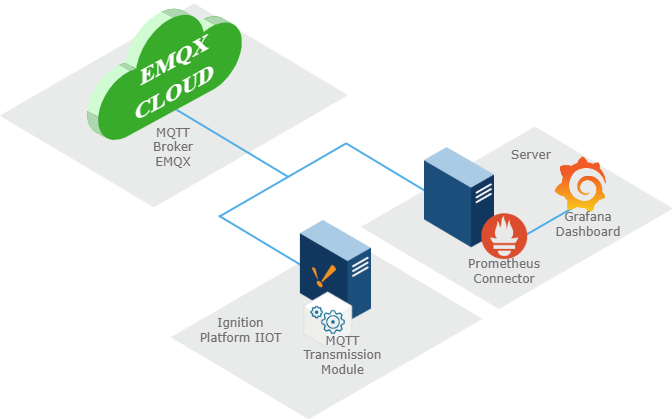
\includegraphics[width=13cm]{Figuras/DiagramaGrafana}}
\caption{Arquitectura de Evaluación de Desempeño}
\label{fig:grafanaconexion}
\end{figure}



La Fig. \ref{fig:grafanaconexion} representa el diagrama de conexiones que permite la evaluación del desempeño de las métricas cualitativas previamente definidas. El flujo de información inicia en la plataforma IIoT Ignition al publicar información generada en la plataforma de entrenamiento hacia un broker MQTT, específicamente el servidor EMQX desplegado en la nube. Posteriormente, un servidor se encarga de consumir estos datos desde el broker y monitorear las métricas mediante su interfaz. Estas métricas son recolectadas por Prometheus, un sistema de monitoreo que realiza consultas periódicas a través de la API del broker, almacenando los resultados en series temporales. 
Finalmente, el visualizador industrial Grafana, se conecta a la base de datos de Prometheus y permite construir paneles interactivos para el análisis histórico, la supervisión en tiempo real y la configuración de alertas basadas en el comportamiento de las métricas del sistema. Esta integración garantiza una visualización eficiente del rendimiento dentro de la plataforma IIoT según las métricas que se describen a continuación.


\subsubsection{Gestión de Tópicos y Sesiones MQTT}

Este conjunto de métricas evalúa la eficiencia del sistema en cuanto a la administración de los tópicos (temas) y las sesiones activas dentro del broker MQTT. Los tópicos representan los canales por los cuales se publica o se suscribe información, y las sesiones reflejan las conexiones activas de los clientes. Una gestión eficiente de estos elementos es fundamental para garantizar un sistema escalable, ordenado y con bajo riesgo de colisiones o redundancias en la comunicación. Además, un número optimizado de suscripciones indica una arquitectura mejor estructurada y alineada con el modelo de datos jerárquico del UNS.

\begin{itemize}
    \item\textbf{deployment\_emqx\_metrics\_topics\_count:} Mide la cantidad total de tópicos activos en el broker EMQX. Cada tópico representa un canal lógico por el que se publican o se reciben mensajes. Un sistema jerárquicamente estructurado tiende a organizar estos tópicos de forma más ordenada y controlada, minimizando redundancias.

    \item\textbf{deployment\_emqx\_sessions\_count:} Corresponde al número de sesiones activas en el broker, es decir, las conexiones cliente-servidor que están intercambiando datos. Esta métrica permite inferir el número de dispositivos o servicios que están interactuando directamente con el broker.
    \item\textbf{deployment\_emqx\_metrics\_subscriptions\_count:} Indica cuántas suscripciones activas existen. Una suscripción ocurre cuando un cliente se registra para recibir los mensajes publicados en un tópico específico. 

\end{itemize}

\begin{figure}[H]
\centerline{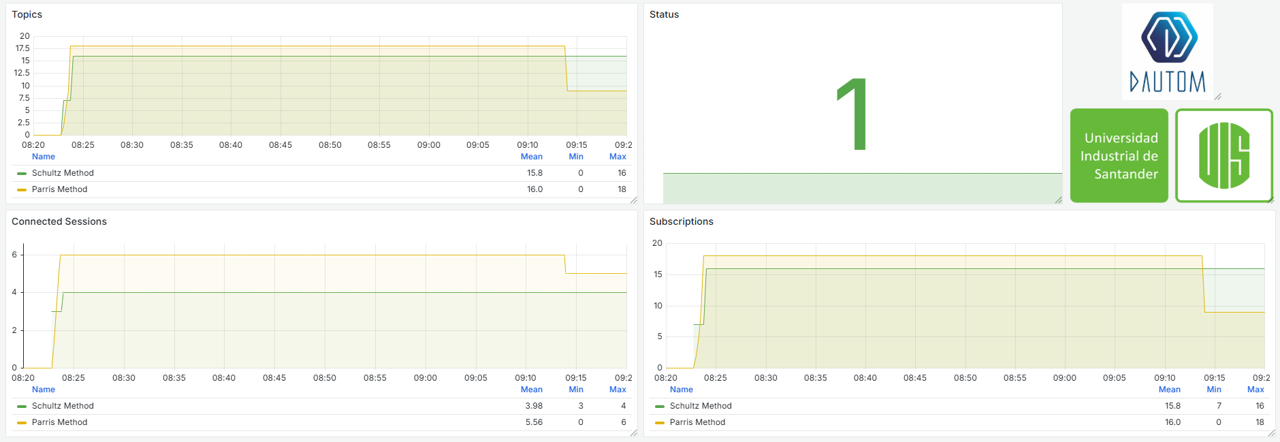
\includegraphics[width=20cm]{Figuras/gf_topics.png}}
\caption{Test de Gestión de Tópicos y Sesiones MQTT}
\label{fig:gf_topics}
\end{figure}

En Grafana se presentan los paneles de visualización con las series temporales como se muestra en la Fig. \ref{fig:gf_topics}. Allí se observan las métricas de gestión de tópicos y sesiones y se distinguen los resultados obtenidos mediante la técnica de Schultz (color verde) y los de la técnica de Parris (color amarillo). Además, se incluyen estadísticas relevantes derivadas del monitoreo continuo para contrastar el comportamiento de ambas arquitecturas.


\begin{table}[H]
\centering
\begin{tabular}{|c|c|c|}
\hline
\textbf{Métrica} & \textbf{Schultz} & \textbf{Parris} \\
\hline
\hspace{30pt}Tópicos\hspace{30pt} &
\hspace{30pt}16\hspace{30pt} & 
\hspace{30pt}18\hspace{30pt} \\
\hline
\hspace{30pt}Sesiones Conectadas\hspace{30pt} &
\hspace{30pt}4\hspace{30pt} & 
\hspace{30pt}6\hspace{30pt} \\
\hline
\hspace{30pt}Suscripciones\hspace{30pt} &
\hspace{30pt}16\hspace{30pt} & 
\hspace{30pt}18\hspace{30pt} \\
\hline
\end{tabular}
\caption{Comparación de Gestión de Tópicos y Sesiones MQTT}
\label{topics_com}
\end{table}



En la comparación de resultados entre las arquitecturas de Schultz y Parris, se observa un comportamiento consistente: Schultz presenta menores valores en las tres métricas como se evidencia en la Tabla \ref{topics_com}. Estos resultados evidencian una arquitectura más contenida y organizada por parte de Schultz. Al estructurar el UNS en distintos niveles jerárquicos, Schultz logra distribuir la responsabilidad de publicación y suscripción, reduciendo la concentración de carga en un único punto. En cambio, Parris, al centralizar toda la información en un solo broker, incrementa inevitablemente la cantidad de tópicos y sesiones necesarias para administrar la misma cantidad de datos, lo que puede dificultar la trazabilidad y escalabilidad del sistema.



\subsubsection{Gestión de Autenticaciones y Autorizaciones}


Este conjunto de métricas permite evaluar el comportamiento del sistema en relación con los procesos de autenticación y autorización de los clientes que interactúan con el broker MQTT. Estas operaciones son fundamentales para garantizar la seguridad, el control de acceso y la gestión eficiente de identidades dentro de arquitecturas IIoT. Analizar estas métricas proporciona una visión clara del volumen de autenticaciones realizadas, las solicitudes de autorización recibidas y las operaciones exitosas de control de acceso como se observa en la Fig.\ref{fig:gf_auten}, permitiendo detectar patrones o posibles vulnerabilidades. 

\begin{itemize}
    \item \textbf{deployment\_emqx\_metrics\_authentication\_success:} Representa el número total de autenticaciones exitosas realizadas por los clientes hacia el broker. Esta métrica es crítica para entender la cantidad de conexiones autenticadas correctamente durante el periodo de evaluación.
    
    \item \textbf{deployment\_emqx\_metrics\_client\_authorize:} Indica la cantidad de solicitudes de autorización recibidas por el broker por parte de los clientes autenticados. Cada vez que un cliente intenta publicar o suscribirse a un tópico, se genera una solicitud que debe ser autorizada, dependiendo de las políticas de control de acceso configuradas.
    
    \item \textbf{deployment\_emqx\_metrics\_authorization\_allow:} Refleja cuántas de esas solicitudes de autorización fueron permitidas según las reglas del sistema. Este valor debe correlacionarse estrechamente con la métrica anterior, y un alto valor sugiere que la mayoría de las operaciones solicitadas por los clientes fueron válidas y seguras.
\end{itemize}

\begin{figure}[h]
\centerline{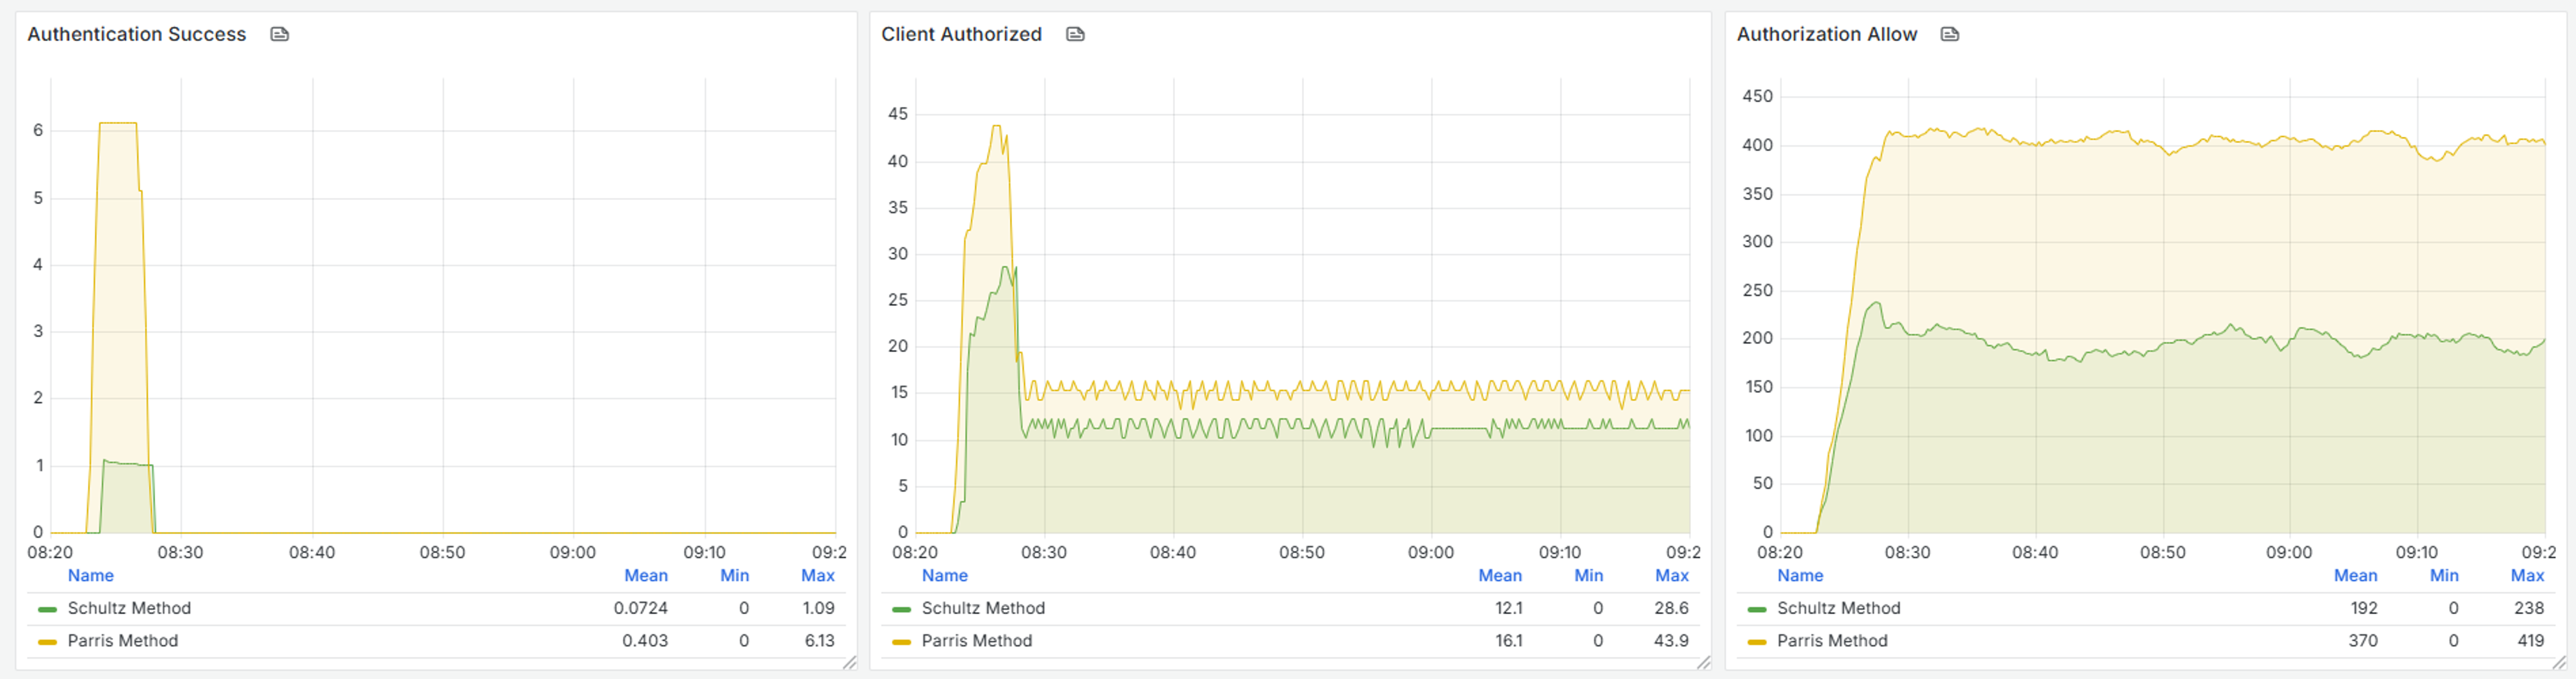
\includegraphics[width=20cm]{Figuras/gf_auten.png}}
\caption{Test de Gestión de Autenticaciones y Autorizaciones}
\label{fig:gf_auten}
\end{figure}


En la evaluación de las métricas relacionadas con autenticación y autorización, se evidencian diferencias notables entre las arquitecturas. La técnica de Parris presentó un mayor número de autenticaciones exitosas como se describe en la tabla \ref{auten_com}. Este comportamiento está directamente relacionado con su arquitectura centralizada, donde todos los clientes deben autenticarse y autorizarse directamente contra un único broker. Esta concentración genera un volumen más alto de operaciones en el punto central, aumentando la complejidad de gestión y potenciales cuellos de botella.

\begin{table}[H]
\centering
\begin{tabular}{|c|c|c|}
\hline
\textbf{Métrica} & \textbf{Schultz} & \textbf{Parris} \\
\hline
\hspace{30pt}Autenticaciones Exitosas\hspace{30pt} &
\hspace{30pt}1\hspace{30pt} & 
\hspace{30pt}6\hspace{30pt} \\
\hline
\hspace{30pt}Clientes Autorizados\hspace{30pt} &
\hspace{30pt}12\hspace{30pt} & 
\hspace{30pt}16\hspace{30pt} \\
\hline
\hspace{30pt}Autorizaciones Permitidas\hspace{30pt} &
\hspace{30pt}192\hspace{30pt} & 
\hspace{30pt}370\hspace{30pt} \\
\hline
\end{tabular}
\caption{Comparación de Gestión de Autenticaciones y Autorizaciones}
\label{auten_com}
\end{table}


Por su parte, la técnica de Schultz, al implementar una arquitectura jerárquica con múltiples niveles de brokers distribuidos, logra desacoplar el tráfico de autenticación, permitiendo que muchas de estas operaciones ocurran de forma intermedia antes de llegar al broker principal. Esto reduce la cantidad de accesos directos y mejora la segmentación de seguridad. Aunque sus métricas reflejan un menor volumen de eventos, este comportamiento implica una mayor eficiencia operativa y una arquitectura más segura y escalable, posicionando a Schultz como una mejor opción en entornos industriales que requieran control granular y tolerancia a fallos.


\subsubsection{Flujo de Datos}
Estas métricas están orientadas a evaluar el volumen de datos que circula a través del broker MQTT durante el funcionamiento de cada arquitectura, permitiendo cuantificar tanto la entrada como la salida de información del sistema a partir de tasas de transferencia promedio por segundo y por minuto. La Fig.\ref{fig:gf_bytes} permite observar con mayor claridad el comportamiento del flujo de datos en escalas de tiempo relevantes para operaciones industriales.

Estas métricas son fundamentales para entender el rendimiento de red y la eficiencia en el intercambio de datos entre productores (Ignition) y consumidores (cliente). Un flujo constante y bien distribuido es indicativo de una arquitectura optimizada tanto para el tráfico entrante como saliente, aspecto esencial en entornos IIoT donde grandes volúmenes de datos deben ser procesados en tiempo real sin generar obstrucciones.

\begin{figure}[H]
\centerline{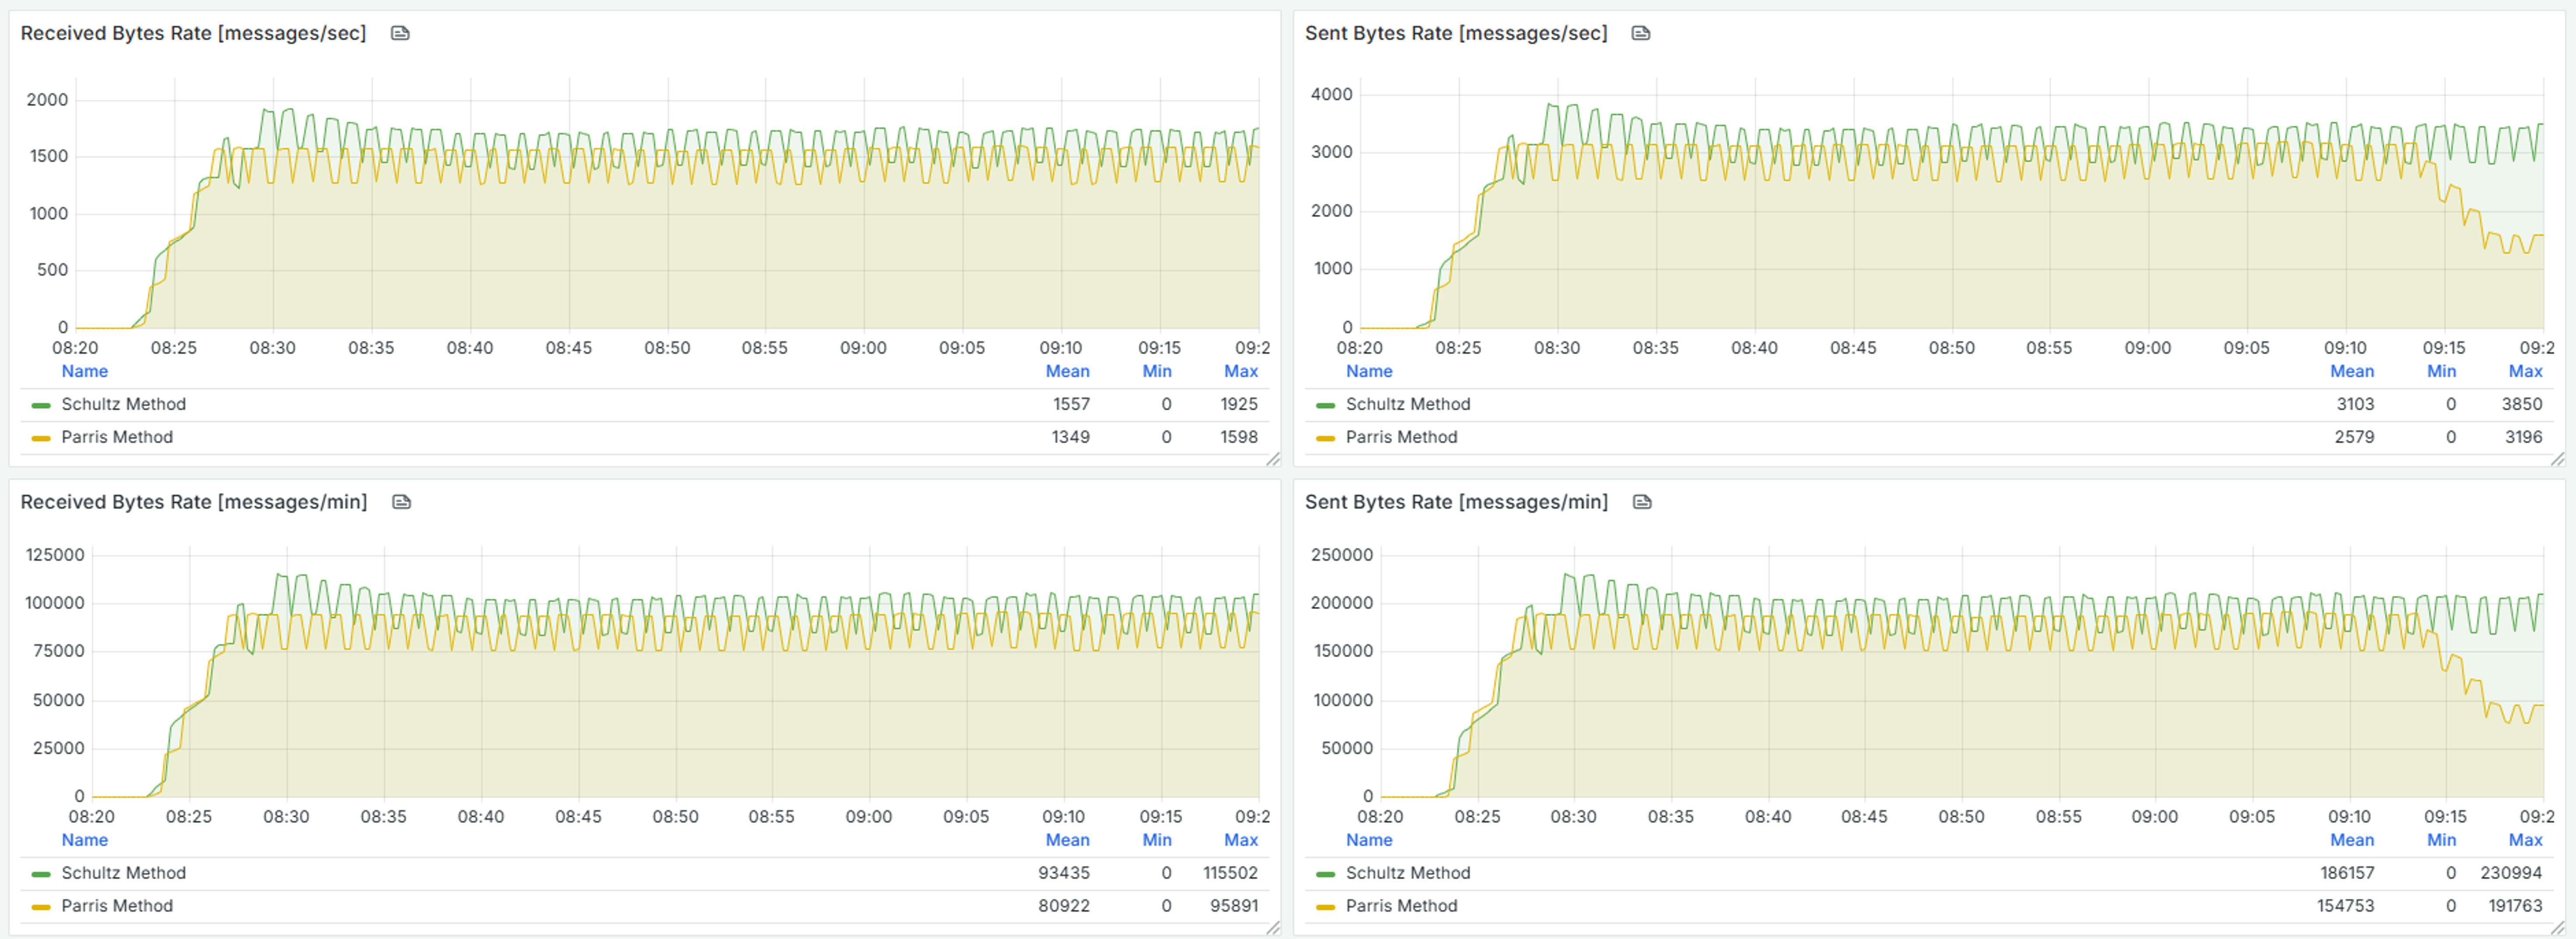
\includegraphics[width=20cm]{Figuras/gf_bytes.png}}
\caption{Test de Flujo de Datos}
\label{fig:gf_bytes}
\end{figure}


\begin{itemize}
    \item \textbf{deployment\_emqx\_metrics\_bytes\_received:} Mide la tasa de bytes recibidos por el broker, calcula la cantidad promedio de bytes recibidos por segundo en ese lapso, proporcionando una visión precisa de la cantidad de datos que el broker recibe desde las plataformas IIoT o dispositivos conectados.
    
    \item \textbf{deployment\_emqx\_metrics\_bytes\_sent:}  Similar a la métrica anterior, pero en este caso se mide la cantidad de bytes enviados por el broker a los clientes conectados para observar la salida de datos hacia las aplicaciones que consumen la información.
    
    \item \textbf{deployment\_emqx\_metrics\_bytes\_received*60:} Esta métrica es similar a la primera, pero escalada a bytes por minuto. Multiplicando la tasa por 60 se obtiene la cantidad total de bytes recibidos en un minuto para facilitar la interpretación de la cantidad de datos en un tiempo mayor y así planificar capacidades de la red.

    \item \textbf{deployment\_emqx\_metrics\_bytes\_sent*60:} Nuevamente, esta métrica mide la tasa de bytes enviados por el broker, pero escalada a bytes por minuto. Es útil para observar el volumen total de datos distribuidos hacia los clientes por minuto, brindando una visión más detallada del rendimiento en intervalos de tiempo más largos.
        
\end{itemize}


Los valores reportados para la tasa de datos recibidos indican que la técnica de Schultz alcanzó una media de 1.557 bytes/seg, frente a los 1.349 bytes/seg obtenidos por Parris como se compara en la tabla \ref{bytes_com} lo que demuestra que Schultz maneja una mayor cantidad de información tanto de entrada como de salida.

\begin{table}[H]
\centering
\begin{tabular}{|c|c|c|}
\hline
\textbf{Métrica} & \textbf{Schultz} & \textbf{Parris} \\
\hline
\hspace{30pt}Bytes Recibidos por Segundo\hspace{30pt} &
\hspace{30pt}1557\hspace{30pt} & 
\hspace{30pt}1349\hspace{30pt} \\
\hline
\hspace{30pt}Bytes Enviados por Segundo\hspace{30pt} &
\hspace{30pt}3103\hspace{30pt} & 
\hspace{30pt}2579\hspace{30pt} \\
\hline
\hspace{30pt}Bytes Recibidos por Minuto\hspace{30pt} &
\hspace{30pt}93435\hspace{30pt} & 
\hspace{30pt}80922\hspace{30pt} \\
\hline
\hspace{30pt}Bytes Enviados por Minuto\hspace{30pt} &
\hspace{30pt}186157\hspace{30pt} & 
\hspace{30pt}154753\hspace{30pt} \\
\hline
\end{tabular}
\caption{Comparación de Flujo de Datos}
\label{bytes_com}
\end{table}


Esta diferencia refleja cómo la arquitectura jerárquica y segmentada de Schultz permite un procesamiento y redistribución de datos más robusto, especialmente al escalar el sistema. Pese a su mayor complejidad en integración, Schultz optimiza el flujo de datos a través de sus múltiples niveles, evitando cuellos de botella. En cambio, aunque la técnica de Parris es más sencilla de integrar, su enfoque centralizado limita el rendimiento general cuando el volumen de datos aumenta. Esto convierte a Schultz en la opción más sólida para escenarios donde se espera alta densidad de tráfico o expansión futura del sistema.




\subsubsection{Gestión de Clientes}

Estas métricas se enfocan en la interacción de los clientes con el broker. Las métricas clave incluyen el número de conexiones establecidas por los clientes y la cantidad de autorizaciones que reciben para interactuar con el broker. Estos indicadores son fundamentales para medir la carga de trabajo del sistema, la eficiencia en la gestión de clientes y la efectividad de los mecanismos de autenticación y autorización. En términos generales, un análisis de estas métricas permite evaluar la capacidad de la infraestructura para manejar múltiples clientes y la velocidad con que se gestionan sus conexiones y autorizaciones. Los resultados se pueden evidenciar en la Fig.\ref{fig:gf_clients}.

\begin{itemize}
    \item \textbf{deployment\_emqx\_metrics\_client\_connect:} Esta métrica mide el número de conexiones de clientes al broker durante el intervalo de tiempo. Representa la cantidad de clientes que logran establecer una conexión exitosa con el broker.

    \item \textbf{deployment\_emqx\_metrics\_client\_authorize:} Mide el número de autorizaciones realizadas para los clientes durante un intervalo de tiempo determinado. Cada vez que un cliente es autenticado y autorizado para acceder a los servicios del broker, esta métrica incrementa.

\end{itemize}

\begin{figure}[H]
\centerline{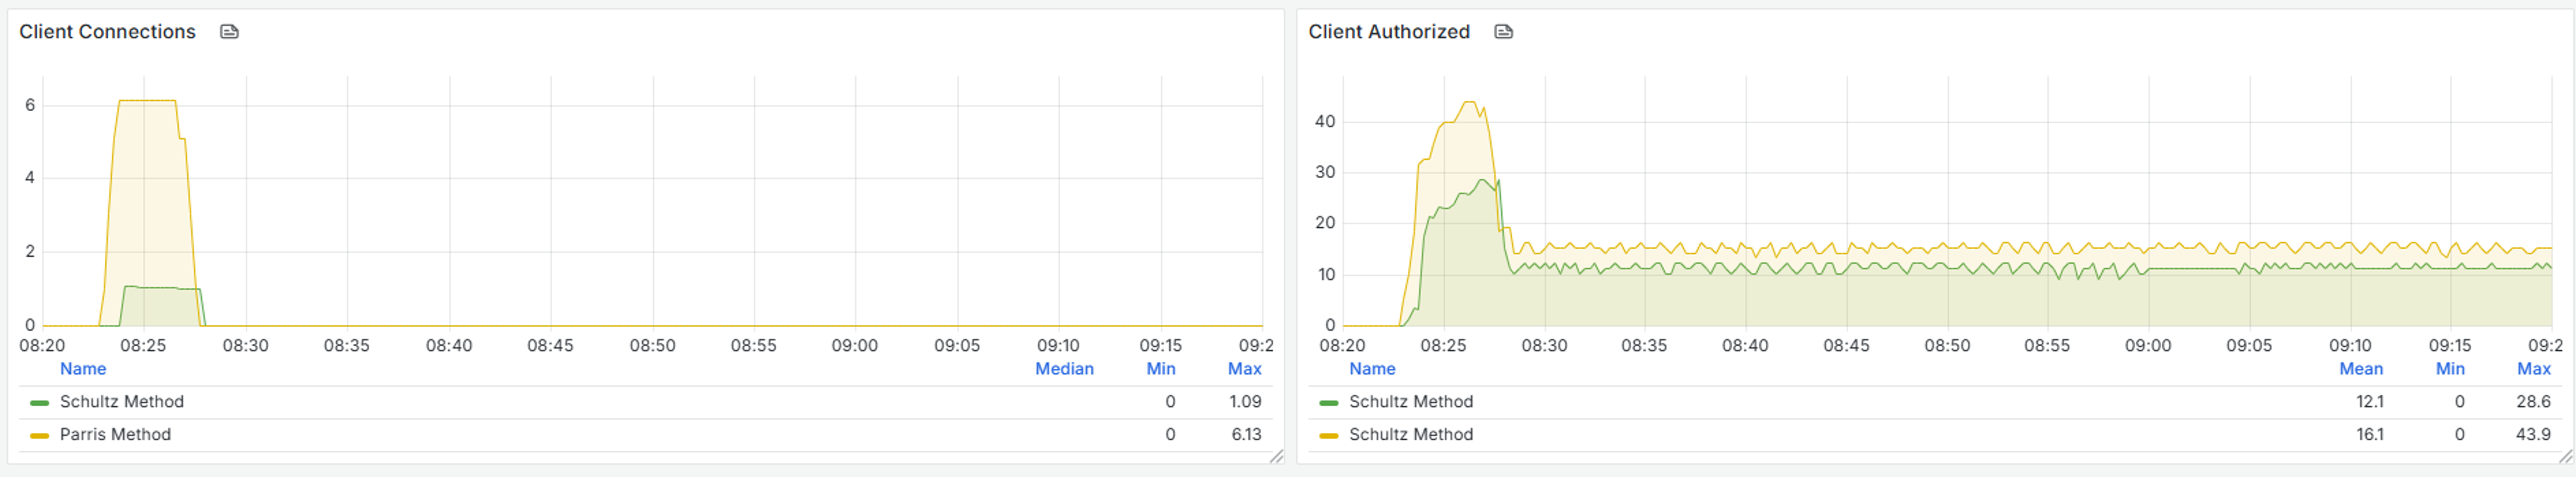
\includegraphics[width=20cm]{Figuras/gf_clients.png}}
\caption{Test de Gestión de Clientes}
\label{fig:gf_clients}
\end{figure}

Los resultados obtenidos en la tabla \ref{clients_com} revelan que la técnica de Schultz muestra una conexión significativamente menor con solo 1 cliente conectado durante el periodo de prueba en comparación con los 6 clientes de Parris. En términos de autorización, Schultz presenta 12 autorizaciones, mientras que Parris alcanza las 16, lo que sugiere que la técnica de Parris maneja una mayor cantidad de clientes conectados y autorizados dentro de los mismos intervalos de tiempo.

\begin{table}[H]
\centering
\begin{tabular}{|c|c|c|}
\hline
\textbf{Métrica} & \textbf{Schultz} & \textbf{Parris} \\
\hline
\hspace{30pt}Clientes Conectados\hspace{30pt} &
\hspace{30pt}1\hspace{30pt} & 
\hspace{30pt}6\hspace{30pt} \\
\hline
\hspace{30pt}Clientes Autorizados\hspace{30pt} &
\hspace{30pt}12\hspace{30pt} & 
\hspace{30pt}16\hspace{30pt} \\
\hline
\end{tabular}
\caption{Comparación de Gestión de Clientes}
\label{clients_com}
\end{table}


En términos generales, estos resultados indican que la técnica de Parris logra gestionar un mayor número de clientes simultáneamente en comparación con Schultz, lo que podría estar relacionado con su arquitectura centralizada que permite una gestión más sencilla de las conexiones y autorizaciones de clientes. Sin embargo, la técnica de Schultz podría ser más adecuada para escenarios donde la gestión de clientes se realiza de manera más autónoma en distintas áreas, lo cual podría generar una carga menor en el broker central.





\subsubsection{Gestión de Mensajes}

Este conjunto de métricas se centra en la actividad relacionada con el tráfico de mensajes dentro del broker. Evalúa tanto la recepción como el envío de mensajes, así como la frecuencia con la que los mensajes son publicados. Estas métricas son esenciales para entender el rendimiento de las arquitecturas IIoT en términos de comunicación, ya que permiten cuantificar la carga de datos que se transmite a través del sistema. Además, ayudan a identificar bloqueos en el flujo de información y permite evaluar la eficiencia del manejo del tráfico de mensajes bajo distintos esquemas de arquitectura.


\begin{itemize}
    \item \textbf{deployment\_emqx\_received\_msg\_rate:} Tasa promedio de mensajes recibidos para indicar cuántos mensajes el broker recibe en promedio en cada segundo dentro de esa ventana temporal.

    \item \textbf{deployment\_emqx\_sent\_msg\_rate:} Tasa promedio de mensajes enviados para reflejar la frecuencia con la que el broker distribuye mensajes a los clientes suscritos.

    \item \textbf{deployment\_emqx\_received\_msg\_rate* 60}: Proyección del total de mensajes recibidos por minuto. Se obtiene multiplicando la tasa por segundo por 60 para obtener una métrica más intuitiva a escala de minutos.

    \item \textbf{deployment\_emqx\_sent\_msg\_rate * 60:} Tasa de mensajes enviados por minuto, derivada del mismo procedimiento. Proporciona una mejor apreciación de la actividad total en el sistema durante períodos más largos.

    \item \textbf{deployment\_emqx\_metrics\_messages\_publish:} Mide la tasa de publicación de mensajes, es decir, la cantidad de mensajes nuevos que son publicados al broker en promedio por segundo durante el intervalo de tiempo.

\end{itemize}

\begin{figure}[H]
\centerline{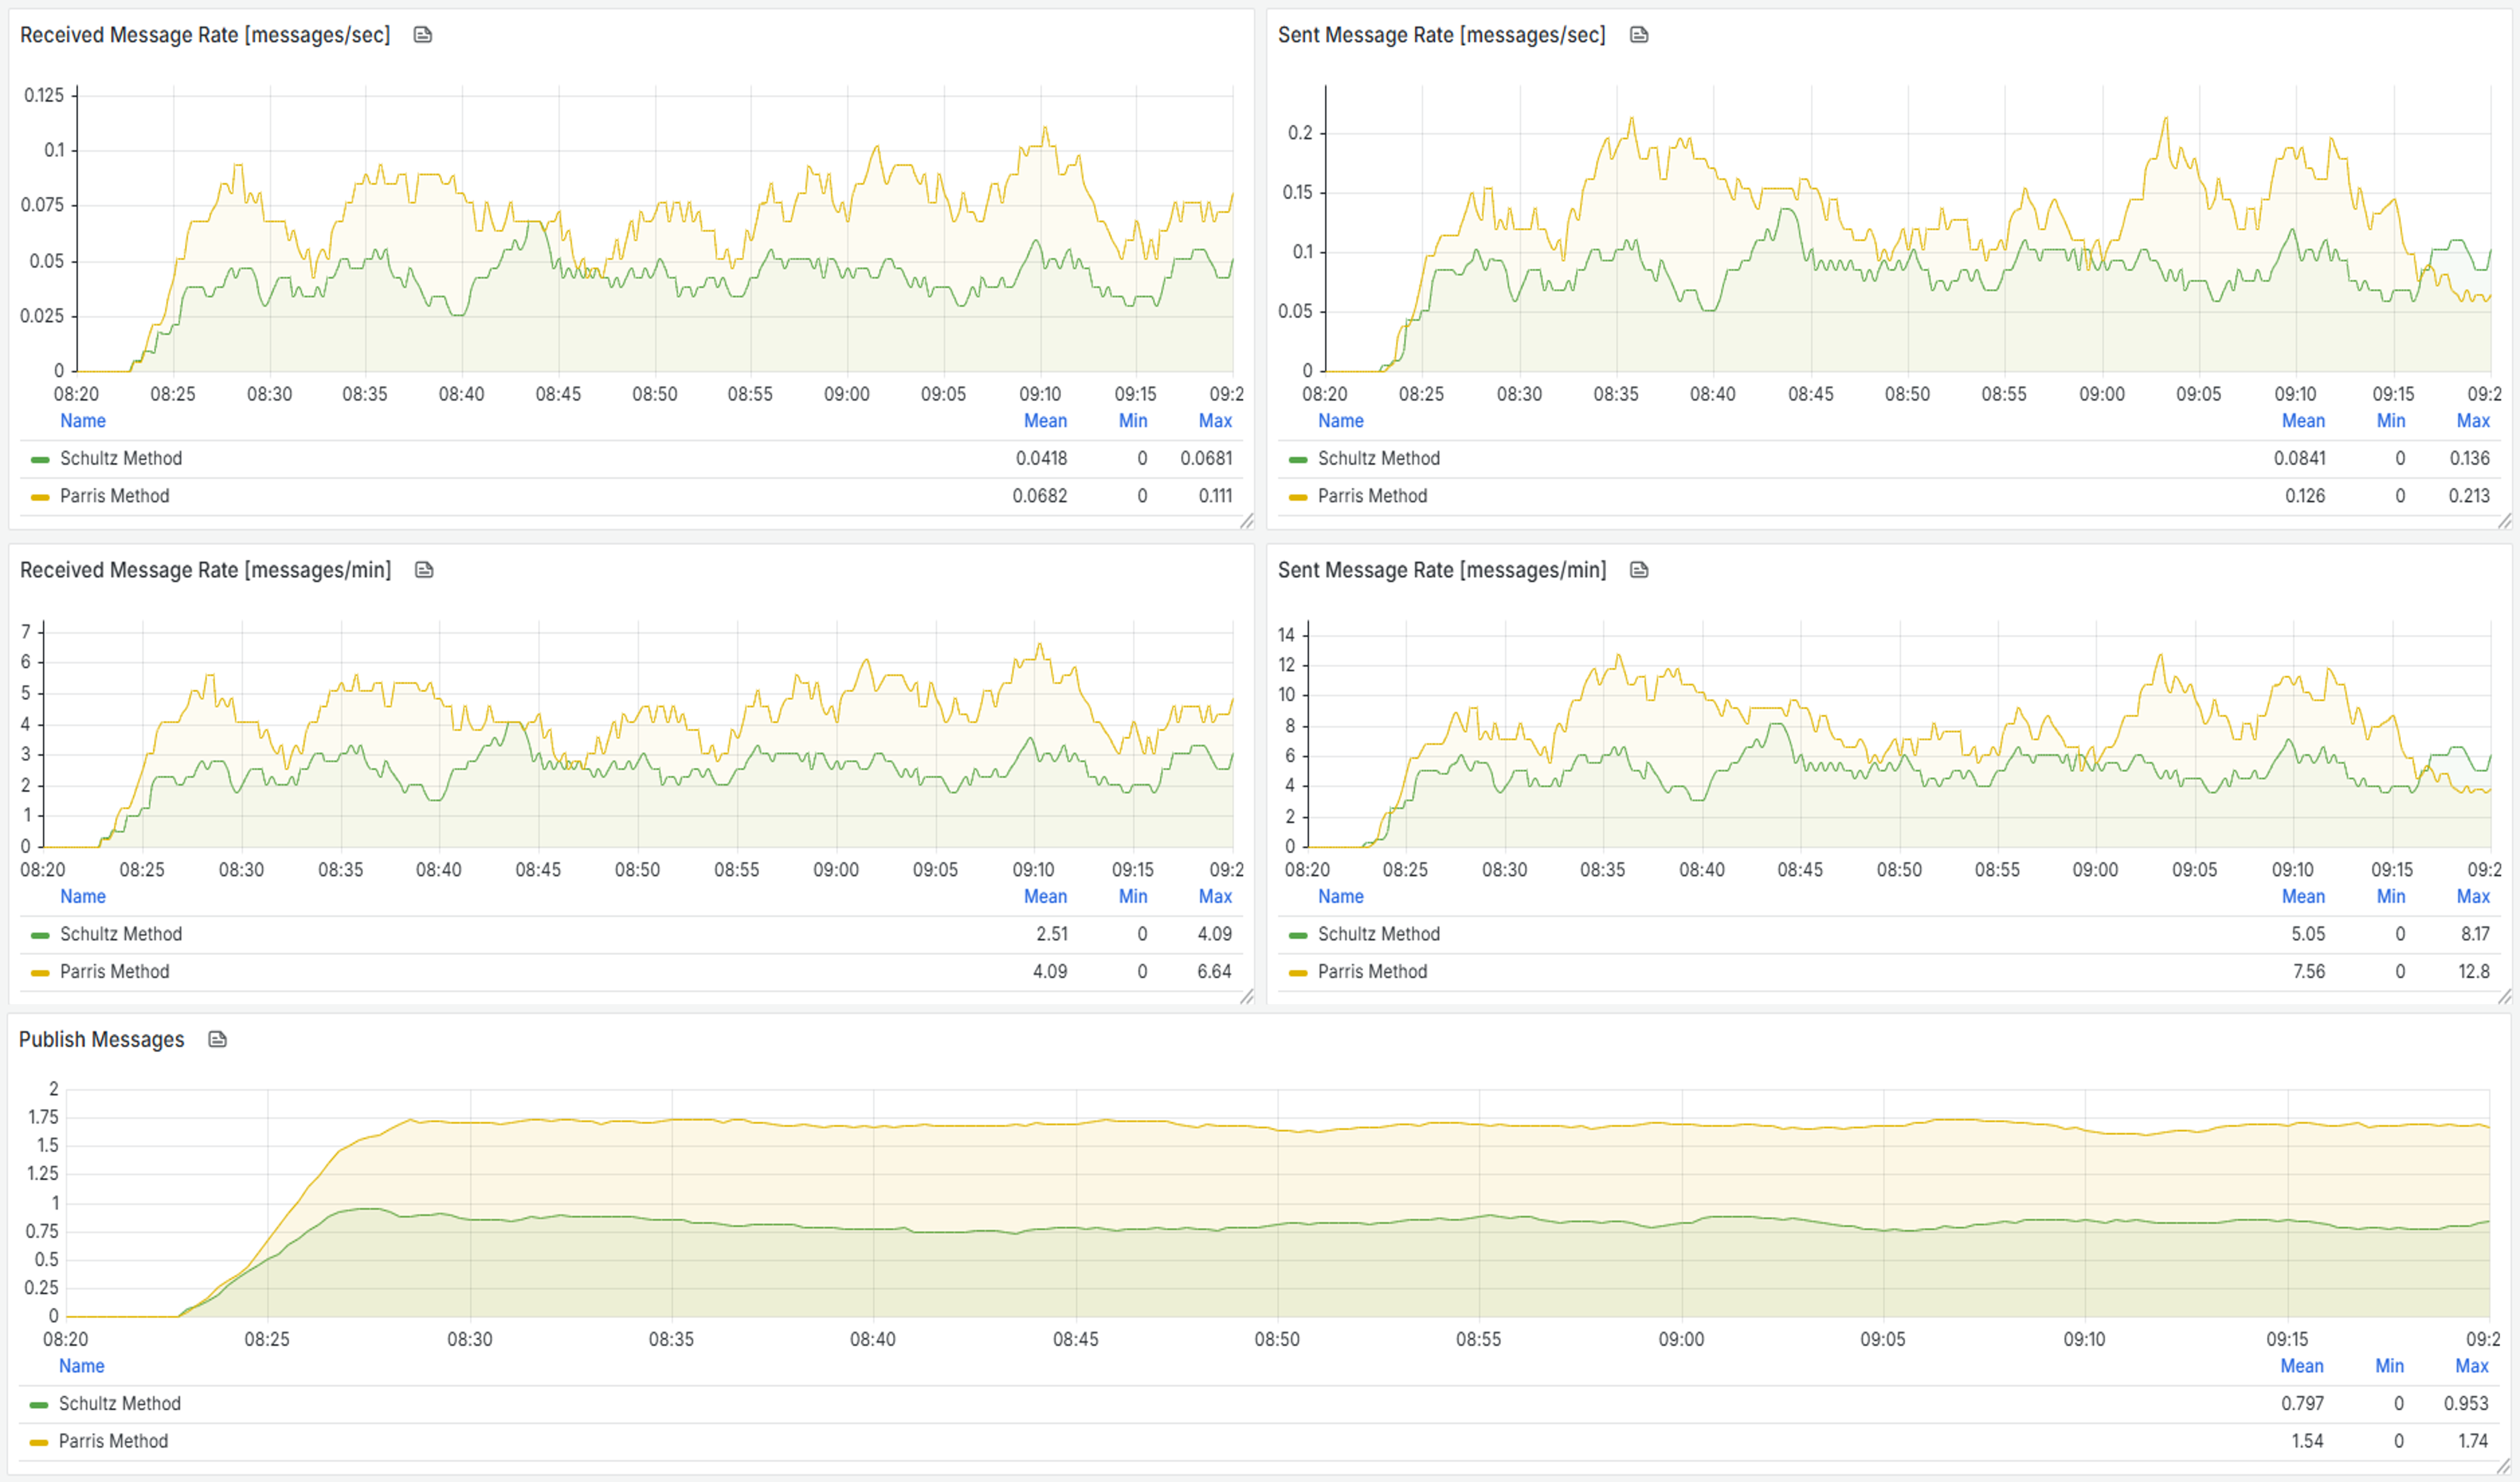
\includegraphics[width=20cm]{Figuras/gf_messages.png}}
\caption{Test de Gestión de Mensajes}
\label{fig:gf_messages}
\end{figure}


En la Fig. \ref{fig:gf_messages} se observan los resultado de la gestión de mensajes en cada una de las métricas definidas. Al comparar ambas arquitecturas, se observa que Parris mantiene una tasa superior tanto en recepción como en envío de mensajes. Los resultados de cada una de las tasas de mensajería se muestran en la tabla \ref{messages_com} a continuación.

\begin{table}[H]
\centering
\begin{tabular}{|c|c|c|}
\hline
\textbf{Métrica} & \textbf{Schultz} & \textbf{Parris} \\
\hline
\hspace{30pt}Mensajes Recibidos por Segundo\hspace{30pt} &
\hspace{30pt}0.0588\hspace{30pt} & 
\hspace{30pt}0.0763\hspace{30pt} \\
\hline
\hspace{30pt}Mensajes Enviados por Segundo\hspace{30pt} &
\hspace{30pt}0.124\hspace{30pt} & 
\hspace{30pt}0.167\hspace{30pt} \\
\hline
\hspace{30pt}Mensajes Recibidos por Minuto\hspace{30pt} &
\hspace{30pt}3.53\hspace{30pt} & 
\hspace{30pt}4.58\hspace{30pt} \\
\hline
\hspace{30pt}Mensajes Enviados por Minuto\hspace{30pt} &
\hspace{30pt}7.45\hspace{30pt} & 
\hspace{30pt}10\hspace{30pt} \\
\hline
\hspace{30pt}Mensajes Publicados\hspace{30pt} &
\hspace{30pt}0.797\hspace{30pt} & 
\hspace{30pt}1.54\hspace{30pt} \\
\hline
\end{tabular}
\caption{Comparación de Gestión de Mensajes}
\label{messages_com}
\end{table}


Estos resultados sugieren que Parris facilita una mayor actividad de mensajería dentro del mismo intervalo de tiempo. Esta diferencia se atribuye al enfoque centralizado de la arquitectura, que permite una difusión más rápida y directa de los mensajes, sin requerir pasos intermedios de agregación o procesamiento. En contraste, la arquitectura Schultz, al segmentar jerárquicamente los niveles de información, puede introducir latencias naturales que impactan la tasa de publicación y distribución de mensajes, aunque podría estar optimizada para casos donde se priorice robustez o filtrado local. 

\subsubsection{Actividad de Paquetes}

Este último grupo comprende métricas orientadas a monitorear el volumen y comportamiento del tráfico de paquetes que circulan entre los clientes y el broker. A diferencia de las métricas de mensajes, que se enfocan en el contenido informativo que se transmite, las métricas de paquetes se centran en los distintos tipos de señales del protocolo MQTT que permiten establecer, mantener y finalizar las conexiones, así como realizar operaciones como suscripciones y publicaciones. 

Estas métricas son fundamentales para caracterizar el nivel de interacción entre clientes y el servidor, evaluar el rendimiento del canal de comunicación y detectar posibles cuellos de botella en la negociación del protocolo.\\~\\

\begin{itemize}
    \item \textbf{rate(deployment\_emqx\_metrics\_packets\_received):} Tasa de recepción de paquetes por segundo. Refleja el flujo constante de datos entrantes hacia el broker, incluyendo todos los tipos de paquetes MQTT.

    \item \textbf{rate(deployment\_emqx\_metrics\_packets\_sent):} Tasa de paquetes enviados por segundo. Mide la capacidad del broker para responder a los clientes o reenviar datos, útil para analizar la carga saliente.

    \item \textbf{increase(deployment\_emqx\_metrics\_packets\_received):} Incremento total de paquetes recibidos durante el intervalo de análisis. Indica la acumulación neta de tráfico entrante.

    \item \textbf{increase(deployment\_emqx\_metrics\_packets\_sent):} Incremento total de paquetes enviados en el periodo observado. Complementa la métrica anterior para reflejar la magnitud de la actividad bidireccional.

    \item \textbf{deployment\_emqx\_metrics\_packets\_subscribe\_received:} Cantidad de paquetes SUBSCRIBE recibidos. Representa solicitudes de suscripción a tópicos por parte de los clientes.

    \item \textbf{deployment\_emqx\_metrics\_packets\_connect:} Número de paquetes CONNECT. Corresponde a los intentos de los clientes por establecer una conexión con el broker.

    \item \textbf{deployment\_emqx\_metrics\_packets\_pingreq\_received:} Cantidad de paquetes PINGREQ recibidos. Usados por los clientes para mantener viva la conexión, especialmente en períodos de inactividad de datos.

\end{itemize}

\begin{figure}[H]
\centerline{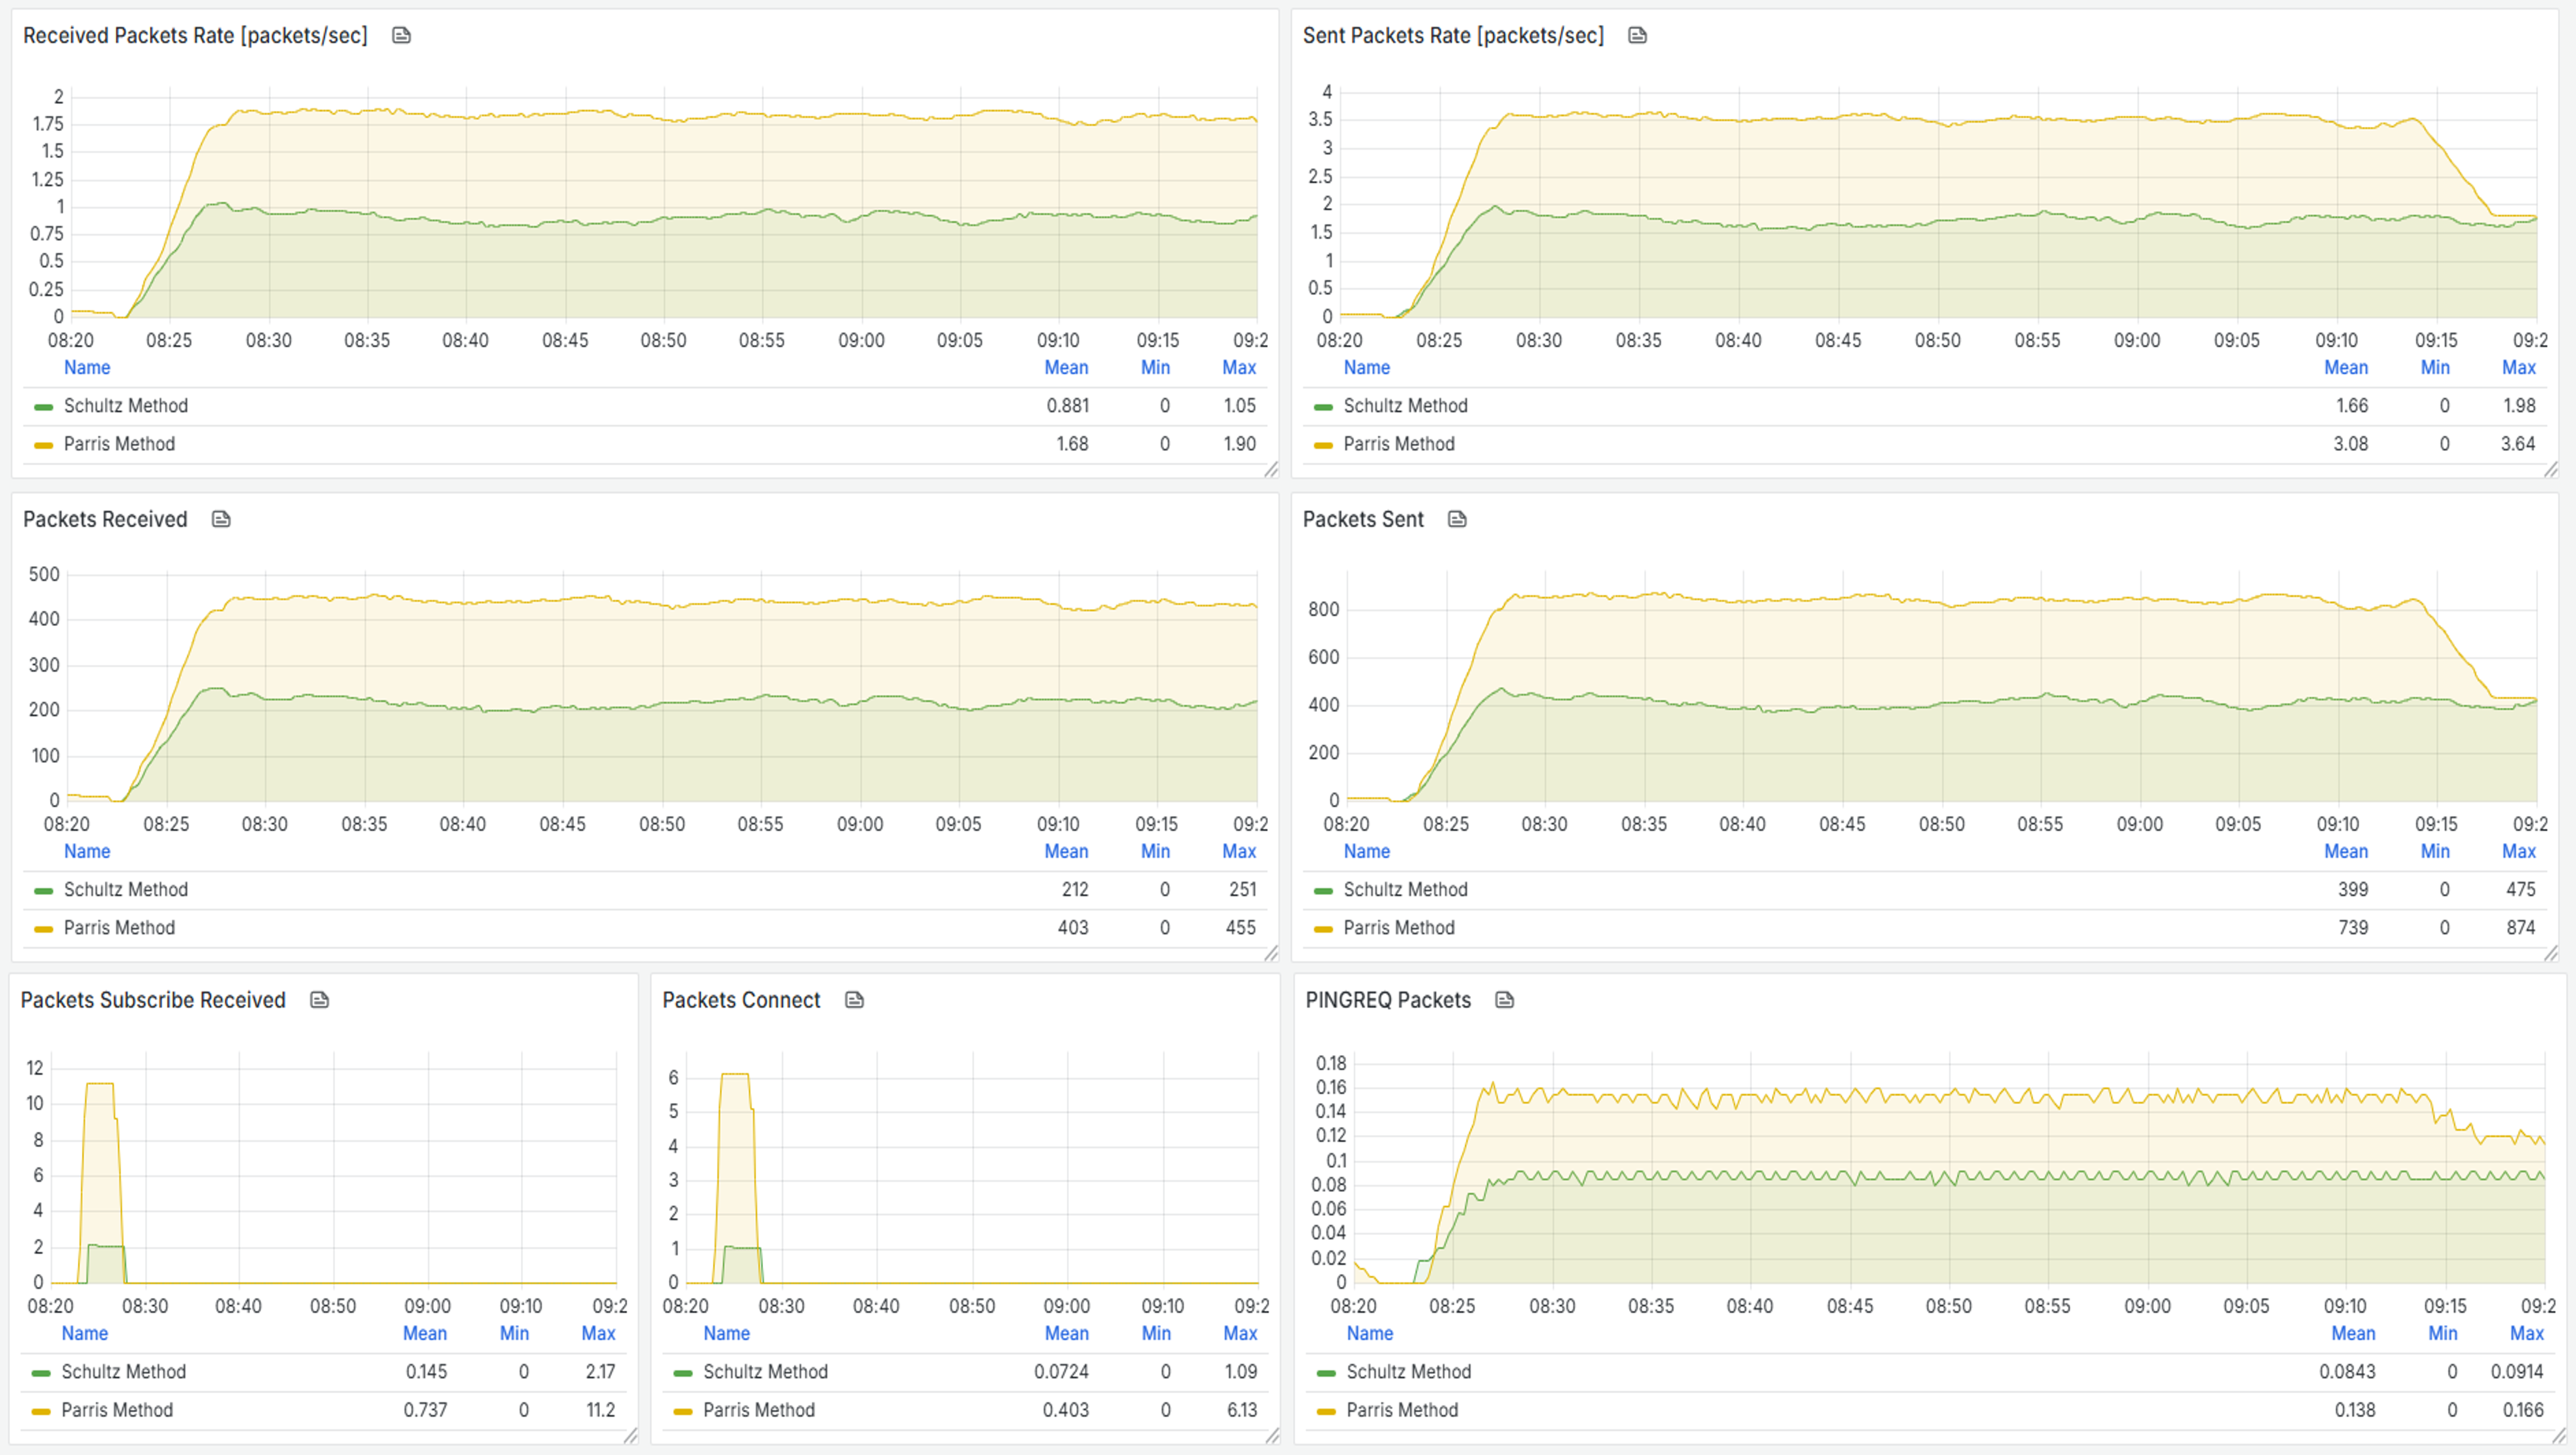
\includegraphics[width=20cm]{Figuras/gf_packets.png}}
\caption{Test de Actividad de Paquetes}
\label{fig:gf_packets}
\end{figure}

Los resultados presentados en la Tabla \ref{packets_com} muestran que la técnica Parris genera una actividad significativamente más intensiva en el intercambio de paquetes MQTT, con una mayor tasa de transmisión y recepción, así como un número más elevado de mensajes asociados a conexiones, suscripciones y mantenimiento de sesión. Este comportamiento indica una mayor frecuencia de interacción entre clientes y servidor, lo que puede traducirse en una respuesta más rápida ante eventos y cambios en el sistema. Tal dinámica resulta especialmente útil en entornos que requieren actualizaciones de estado en tiempo real o una sincronización continua entre múltiples dispositivos.

\begin{table}[H]
\centering
\begin{tabular}{|c|c|c|}
\hline
\textbf{Métrica} & \textbf{Schultz} & \textbf{Parris} \\
\hline
\hspace{30pt}Paquetes Recibos por Segundo\hspace{30pt} &
\hspace{30pt}0.881\hspace{30pt} & 
\hspace{30pt}1.68\hspace{30pt} \\
\hline
\hspace{30pt}Paquetes Enviados por Segundo\hspace{30pt} &
\hspace{30pt}1.66\hspace{30pt} & 
\hspace{30pt}3.08\hspace{30pt} \\
\hline
\hspace{30pt}Paquetes Payload Recibidos\hspace{30pt} &
\hspace{30pt}212\hspace{30pt} & 
\hspace{30pt}403\hspace{30pt} \\
\hline
\hspace{30pt}Paquetes Payload Enviados\hspace{30pt} &
\hspace{30pt}399\hspace{30pt} & 
\hspace{30pt}739\hspace{30pt} \\
\hline
\hspace{30pt}Paquetes de Subscripción Recibidos\hspace{30pt} &
\hspace{30pt}2\hspace{30pt} & 
\hspace{30pt}11\hspace{30pt} \\
\hline
\hspace{30pt}Paquetes de Conexión\hspace{30pt} &
\hspace{30pt}1\hspace{30pt} & 
\hspace{30pt}6\hspace{30pt} \\
\hline
\hspace{30pt}Paquetes PINGREQ\hspace{30pt} &
\hspace{30pt}0.0843\hspace{30pt} & 
\hspace{30pt}0.138\hspace{30pt} \\
\hline
\end{tabular}
\caption{Comparación de Actividad de Paquetes}
\label{packets_com}
\end{table}


En contraste, la técnica de Schultz genera un tráfico de paquetes más moderado con una comunicación con menor intensidad. Esta característica representa una ventaja en términos de eficiencia en el uso de la red y consumo de recursos, especialmente en entornos con conectividad limitada o donde se prioriza la estabilidad sobre la inmediatez.No obstante, considerando la mayor capacidad de respuesta y el flujo de información sostenido que ofrece la técnica Parris según estas métricas, sería recomendable su implementación en contextos donde la criticidad operativa y la necesidad de monitoreo continuo sean factores clave.



\subsection {Síntesis y Recomendaciones de Implementación}

El análisis comparativo entre las técnicas Schultz y Parris, sustentado en las métricas cualitativas y cuantitativas, permite establecer un panorama integral sobre su desempeño y aplicabilidad en distintos entornos industriales y académicos. La tabla \ref{all_com} refleja que la técnica Schultz mostró un rendimiento más favorable en aspectos como la resiliencia, seguridad, facilidad de implementación, escalabilidad y eficiencia en la gestión de autenticaciones, clientes, tópicos y sesiones MQTT. Esto sugiere que Schultz es adecuada para entornos donde se prioriza la estabilidad operativa, la predictibilidad del comportamiento del sistema, y donde las capacidades de despliegue deben ser rápidas y confiables. En contraste, la técnica Parris demostró fortalezas en dimensiones como integración con otros servicios, flexibilidad para adaptarse a distintos escenarios de comunicación, y un desempeño más eficiente en la gestión dinámica de mensajes y paquetes. Estos resultados la posicionan como una alternativa más apropiada para arquitecturas en evolución, entornos distribuidos con alta interacción entre componentes, o soluciones que requieren una rápida adaptabilidad a cambios en el sistema.

\begin{table}[H]
\centering
\begin{tabular}{|c|c|c|}
\hline
\textbf{Métrica} & \textbf{Schultz} & \textbf{Parris} \\
\hline

\hspace{20pt}Integracion\hspace{20pt} &
\hspace{20pt}{\color{red}\ding{55}}\hspace{20pt} & 
\hspace{2pt}{\color{green}\ding{51}}\hspace{20pt}\\
\hline

\hspace{20pt}Resiliencia\hspace{20pt} &
\hspace{20pt}{\color{green}\ding{51}}\hspace{20pt} & 
\hspace{20pt}{\color{red}\ding{55}}\hspace{20pt} \\
\hline

\hspace{20pt}Flexibilidad\hspace{20pt} &
\hspace{20pt}{\color{red}\ding{55}}\hspace{20pt} & 
\hspace{2pt}{\color{green}\ding{51}}\hspace{20pt}\\
\hline

\hspace{20pt}Seguridad\hspace{20pt} &
\hspace{20pt}{\color{green}\ding{51}}\hspace{20pt} & 
\hspace{20pt}{\color{red}\ding{55}}\hspace{20pt} \\
\hline

\hspace{20pt}Implementación\hspace{20pt} &
\hspace{20pt}{\color{green}\ding{51}}\hspace{20pt} & 
\hspace{20pt}{\color{red}\ding{55}}\hspace{20pt} \\
\hline

\hspace{20pt}Escalabilidad\hspace{20pt} &
\hspace{20pt}{\color{green}\ding{51}}\hspace{20pt} & 
\hspace{20pt}{\color{red}\ding{55}}\hspace{20pt} \\
\hline

\hspace{20pt}Gestion de Topicos y Sesiones MQTT \hspace{20pt} &
\hspace{20pt}{\color{green}\ding{51}}\hspace{20pt} & 
\hspace{20pt}{\color{red}\ding{55}}\hspace{20pt} \\
\hline

\hspace{20pt}Gestion de Autenticaciones y Autorizaciones\hspace{20pt} &
\hspace{20pt}{\color{green}\ding{51}}\hspace{20pt} & 
\hspace{20pt}{\color{red}\ding{55}}\hspace{20pt} \\
\hline

\hspace{20pt}Flujo de Datos\hspace{20pt} &
\hspace{20pt}{\color{green}\ding{51}}\hspace{20pt} & 
\hspace{20pt}{\color{red}\ding{55}}\hspace{20pt} \\
\hline

\hspace{20pt}Gestion de Clientes\hspace{20pt} &
\hspace{20pt}{\color{green}\ding{51}}\hspace{20pt} & 
\hspace{20pt}{\color{red}\ding{55}}\hspace{20pt} \\
\hline

\hspace{20pt}Gestion de Mensajes\hspace{20pt} &
\hspace{20pt}{\color{red}\ding{55}}\hspace{20pt} &
\hspace{20pt}{\color{green}\ding{51}}\hspace{20pt} \\
\hline

\hspace{20pt}Actividad de Paquetes\hspace{20pt} &
\hspace{20pt}{\color{red}\ding{55}}\hspace{20pt} &
\hspace{20pt}{\color{green}\ding{51}}\hspace{20pt} \\
\hline

\end{tabular}
\caption{Síntesis de Comparación entre Schultz y Parris}
\label{all_com}
\end{table}


En síntesis, Schultz se presenta como la opción más robusta y sencilla para implementaciones en ambientes críticos, controlados o con restricciones de seguridad y recursos, mientras que Parris resulta ideal para proyectos que buscan flexibilidad, interacción con múltiples sistemas y optimización en el flujo de datos, particularmente en fases de expansión tecnológica o integración con plataformas externas. La elección entre ambas dependerá entonces de la etapa del proyecto, la infraestructura disponible y los objetivos operativos del sistema.



%%\cleardoublepage


%\begin{comment}
    

%\addtocounter{chapter}{-1}
\chapter{Conclusiones}
\label{Cap_AnalisisResultados}
\textit{Presenta las conclusiones más relevantes y propone una línea para la continuación del trabajo de investigación}
\vfill
\renewcommand{\mtctitle}{Contenido}  
\minitoc
\newpage

\cleardoublepage
\end{comment}

\section{Conclusiones}

% Primer objetivo
La revisión del estado del arte del concepto de UNS permitió comprender a profundidad su papel como pieza clave en la convergencia de tecnologías de información (IT) y operación (OT) dentro de los entornos industriales modernos. Se evidenció que el UNS no es simplemente una técnica de integración, sino una filosofía de diseño que reorganiza la forma en que los datos fluyen, se acceden y se gestionan en tiempo real, promoviendo la estandarización, la interoperabilidad y la contextualización a lo largo de toda la arquitectura digital industrial. Este enfoque rompe con los esquemas tradicionales basados en silos de información y abre paso a un modelo en el que todos los actores humanos, máquinas, software y procesos tienen una visión común y actualizada del sistema.

Además, al identificar y comparar las distintas interpretaciones, ventajas y limitaciones del UNS, se logró establecer una base conceptual sólida que sirvió como punto de partida para las siguientes etapas del estudio. El análisis crítico de métodos como los propuestos por David Schultz y Matthew Parris, permitió contrastar enfoques jerárquicos y funcionales, rescatando elementos clave para un diseño efectivo. Este ejercicio ayudó a delimitar el alcance de la investigación, seleccionando los métodos como referencias prácticas para la implementación experimental en la plataforma de entrenamiento IIoT.


% Segundo objetivo
La definición de métricas de evaluación cualitativas y cuantitativas fueron instrumentos de análisis para valorar el comportamiento de las arquitecturas UNS en entornos de simulación. Las métricas cualitativas como integración, resiliencia, flexibilidad, seguridad, implementación y escalabilidad permitieron evaluar dimensiones críticas del diseño, destacando la capacidad de las técnicas UNS para sostener flujos de datos robustos, adaptarse a cambios en tiempo real y facilitar la integración de nuevos elementos tecnológicos sin afectar la operación del sistema. Estas métricas ofrecieron una revisión del desempeño arquitectónico más allá de los simples indicadores técnicos.

Por otro lado, las métricas cuantitativas centradas en la estructura de topics, sesiones activas, autenticaciones, flujos de datos, gestión de clientes y actividad de mensajes MQTT permitieron medir con precisión aspectos operativos relevantes de cada implementación. Gracias a estas métricas, se pudo observar el comportamiento del sistema ante distintos escenarios de carga, tráfico y número de dispositivos conectados. La obtención de estos datos aportó objetividad al análisis comparativo entre métodos UNS, posibilitando una toma de decisiones basada en evidencia técnica. Así, las métricas diseñadas se consolidaron como herramientas clave para evaluar y optimizar arquitecturas UNS futuras.



% Tercer objetivo:

La implementación de los métodos Schultz y Parris en la plataforma Ignition permitió contrastar dos enfoques reconocidos para la estructuración del Unified Namespace. El método Schultz, al organizar jerárquicamente los datos en función del modelo físico y semántico de la planta, ofreció claridad en la navegación del namespace, facilitando la identificación de dispositivos, procesos y valores asociados. Su diseño promovió la estandarización del nombre de los tópicos, lo que redujo la complejidad operativa y mejoró la sostenibilidad del sistema a largo plazo. En la práctica, demostró ser altamente efectivo en escenarios donde la prioridad es la trazabilidad de activos y la consistencia de datos.

El método Parris, en cambio, ofreció una perspectiva más funcional, orientada a reflejar los flujos de proceso y las operaciones de negocio dentro del namespace. Su implementación permitió mapear el comportamiento de sistemas complejos de forma más dinámica y flexible, adaptándose mejor a entornos donde los procesos cambian con mayor frecuencia. Esta característica resultó valiosa para visualizar flujos de trabajo y asociar eventos operativos con su contexto de producción. El análisis comparativo entre ambos métodos evidenció que la elección del enfoque UNS debe responder a las necesidades específicas de cada planta, priorizando ya sea la estabilidad jerárquica o la agilidad funcional.


% Cuarto objetivo:
Mediante la incorporación de los dispositivos industriales de la plataforma de entrenamiento IIoT, conectados a través de un broker MQTT, se simularon condiciones reales de operación para evaluar la robustez de la infraestructura UNS. Se comprobó que el protocolo MQTT Sparkplug B ofrece ventajas notables en cuanto a gestión del estado de los dispositivos, retención de datos, supervisión de la conexión y estandarización del payload, lo cual facilitó la integración de los datos en el namespace. Así, se validó la utilidad del protocolo como base sólida para entornos industriales modernos.

Finalmente, se logró evaluar el desempeño de cada implementación mediante pruebas controladas en la plataforma IIoT desarrollada. Estas pruebas incluyeron análisis en tiempo real de los datos publicados, verificación del cumplimiento de la estructura de nombres, evaluación de la carga del broker, y monitoreo del comportamiento ante eventos disruptivos. Se evidenció que ambas implementaciones UNS fueron funcionales y capaces de sostener flujos de información estables, pero cada una mostró ventajas particulares: mientras el método Schultz sobresalió en organización y claridad del namespace, el método Parris ofreció mayor flexibilidad para representar flujos operativos dinámicos.

Los resultados de las métricas cualitativas y cuantitativas se integraron para obtener una visión completa del rendimiento del sistema, destacando cómo el diseño del namespace influye directamente en la escalabilidad, trazabilidad y facilidad de uso de la plataforma. Esta evaluación permitió validar los beneficios del UNS como habilitador de arquitecturas IIoT, y al mismo tiempo identificar oportunidades de mejora para futuras implementaciones. En conjunto, la plataforma de entrenamiento sirvió como entorno de validación efectivo, permitiendo experimentar en condiciones controladas con resultados extrapolables a escenarios industriales reales. Así, se demostró que el uso de técnicas UNS, correctamente implementadas y evaluadas, puede acelerar la adopción de tecnologías digitales avanzadas en el sector industrial hacia la transformación digital.


\section{Trabajo futuro}

La línea de este trabajo de investigación continúa con la implementación de un UNS en un entorno industrial real para validar su desempeño bajo condiciones operativas no simuladas. Además, se sugiere desarrollar una nueva técnica de diseño que combine las ventajas de los métodos Schultz y Parris, buscando un enfoque más equilibrado entre estructura jerárquica, escalabilidad, resiliencia y flexibilidad en la gestión de datos IIoT.
   
  
\cleardoublepage






%\color{black}

\newpage
% Referencias
\printbibliography[title={Referencias}]
\cleardoublepage

% Anexos
\section*{Anexo A: Conversación completa del flujo de consulta integrado}
\phantomsection
\addcontentsline{toc}{section}{Anexo A: Conversación completa del flujo de consulta integrado}
\label{anexo:conversacion_flujo}

Este anexo reproduce la conversación de la Sección~\ref{flujoconsultaintegrado}, ejecutada en Claude Desktop con los servidores \texttt{uns-mcp} y \texttt{mes-history-mcp} conectados. Se incluye completa y sin cambios, con la pregunta del usuario y la respuesta del LLM tal como las exportó el cliente. La exportación original en PDF se conserva en el repositorio del libro como \texttt{conversacion\_flujo.pdf}.

\fichaconsulta{Combinada (tiempo real e histórica)}{Hola, ¿cómo va la Linea A de Empaque Trigo ahora mismo, y cómo se compara su OEE con el de la última semana?}{\desafio{D2.1} y \desafio{D2.2}, requerimiento \req{R3}}{\texttt{get\_context} (\texttt{uns-mcp}, contexto \texttt{mes}) y \texttt{get\_oee\_history} (\texttt{mes-history-mcp})}{Claude Desktop, 24 de septiembre de 2026, 16:57}

\noindent\textbf{Respuesta del sistema}\par\smallskip

\begin{quote}
\small

\textbf{Línea A de Empaque Trigo en este momento (16:57)}

La línea está en marcha (\texttt{State} = 2) y las tres celdas (Empacadora 1, Empacadora 2 y Enfardadora) reportan \texttt{Running}. Está ejecutando la orden WO91 (corrida 354), producto Trigo -- Libra -- 24 bolsas por fardo, que arrancó a las 16:31:42.

En los 26 minutos de corrida (\texttt{RunTime} = 1565 s) lleva 129 fardos buenos, sin desperdicio y sin paros. Con la velocidad estándar de 5 fardos/min, la meta a esta hora es 130,4 fardos. Eso da:

\medskip
\begin{tabular}{@{}lc@{}}
\hline
\textbf{Indicador} & \textbf{Ahora (corrida 354)} \\
\hline
Disponibilidad & 100 \% \\
Rendimiento & 98,9 \% (129 / 130,4) \\
Calidad & 100 \% \\
OEE & 98,9 \% \\
\hline
\end{tabular}
\medskip

Hice el cálculo a mano a partir de \texttt{GoodCount}, \texttt{RunTime} y \texttt{StandardRate}, y coincide con los tags \texttt{OEE} y \texttt{Performance}, que esta vez sí se están actualizando en tiempo real (\texttt{timestamp} 16:57:48), no quedaron congelados al inicio. De la orden faltan 871 fardos. Al ritmo actual (unos 297 fardos/h) terminaría hacia las 19:53, dos minutos después del fin programado (19:51).

\textbf{Comparación con la última semana (17--24 sep)}

Hubo 18 corridas cerradas. Las 15 corridas de turno regular (310--324) dan una referencia limpia. Las otras tres son atípicas: la 346 duró 17,5 h con un rendimiento de apenas 27 \% (OEE 26,5 \%), y la 349 y la 353 duraron menos de 3 minutos cada una, así que parecen pruebas.

\medskip
\begin{tabular}{@{}lcccc@{}}
\hline
 & \textbf{OEE} & \textbf{Disp.} & \textbf{Rend.} & \textbf{Calidad} \\
\hline
Promedio semana (15 turnos regulares) & 80,6 \% & 95,8 \% & 85,8 \% & 98,2 \% \\
Rango semanal & 71,1 \% -- 91,4 \% & & & \\
Ahora & 98,9 \% & 100 \% & 98,9 \% & 100 \% \\
\hline
\end{tabular}
\medskip

La corrida actual va unos 18 puntos por encima del promedio semanal y supera la mejor corrida de la semana (322, 91,4 \%). La diferencia viene sobre todo del rendimiento: la semana rondó el 86 \% y ahora está casi en el estándar.

Hay que tomar esta comparación con cautela. La corrida lleva solo 26 minutos, y las de la semana duraron entre 2,5 y 4 horas, tiempo en el que se acumulan paros (la disponibilidad bajó a 89--93 \% en seis de ellas) y desperdicio (entre 1 \% y 3 \%). Una cifra al inicio de la corrida suele ser optimista. Si incluyo la corrida 346, el promedio semanal cae a 78,2 \%, y ponderado por duración a 67,1 \%.

Dos detalles menores de los datos. El valor de OEE que guarda la base del MES para la corrida 354 (98,47 \%) va un poco rezagado frente al tag en vivo (98,91 \%), algo normal porque el histórico se actualiza con menos frecuencia. Además, \texttt{Line/Cycle Time} marca 10 s, pero con 5 fardos/min el ciclo estándar sería de 12 s. Conviene revisar qué representa ese tag antes de usarlo en algún cálculo.
\end{quote}

\cleardoublepage
\section*{Anexo B: Banco de preguntas de la validación}
\phantomsection
\addcontentsline{toc}{section}{Anexo B: Banco de preguntas de la validación}
\label{anexo:banco_preguntas}

Este anexo reproduce el banco de 25 preguntas de la Sección~\ref{disenoevaluacion}. Para cada una se indica su categoría, el desafío que pone a prueba, la Tool que debería usar el modelo, la respuesta de referencia con la forma en que se calculó, y la respuesta del sistema en cada una de las tres ejecuciones con su veredicto, su latencia y su puntuación de calidad semántica. Las fechas relativas se calcularon respecto al día de prueba \textcolor{blue}{[fecha]}.

% ------------------------------------------------------------------
% Ejemplo de uso (se reemplaza por las 25 preguntas cuando estén ejecutadas).
% ------------------------------------------------------------------
\fichapregunta{1}{Tiempo real}{\textcolor{blue}{[texto de la pregunta]}}{\textcolor{blue}{[D1.3]}}{\texttt{get\_equipment\_status}}{\textcolor{blue}{[respuesta de referencia]}}{\textcolor{blue}{[lectura de tags de Ignition antes de la pregunta]}}
\ejecucion{1}{\textcolor{blue}{[respuesta]}}{\textcolor{blue}{[correcta/incorrecta]}}{\textcolor{blue}{[ ]}}{\textcolor{blue}{[ / / ]}}
\ejecucion{2}{\textcolor{blue}{[respuesta]}}{\textcolor{blue}{[correcta/incorrecta]}}{\textcolor{blue}{[ ]}}{\textcolor{blue}{[ / / ]}}
\ejecucion{3}{\textcolor{blue}{[respuesta]}}{\textcolor{blue}{[correcta/incorrecta]}}{\textcolor{blue}{[ ]}}{\textcolor{blue}{[ / / ]}}

\cleardoublepage

\end{document}